The classification of jets originated from a quark or a gluon is useful for improving the SM measurements and searches for BSM physics at the LHC.  According to the QCD,  gluons are in the adjoint representation of the $SU(3)$ gauge group thus carry both colour and anti-colour quantum numbers, whereas quarks are in the fundamental representation and have only a single colour number~\cite{ALTARELLI1977298}. As a result, a gluon-initiated jet (gluon-jet) tend to have more constituents and a broader radiation pattern than a quark-initiated jet (quark-jets). 

The manifestation of colour charges is intrinsic to quarks and gluons; however, the confinement phenomenon inherent in QCD theory indicates that only colour neutral hadrons can be observed in the detector. Such principle brings significant challenges for the identification of quark- or gluon-jets in ATLAS. The identification method relies on the number of charged tracks within the jets and the reconstruction algorithm for it. The calibration described in this paper demonstrates the measurement of the tagging efficiencies of the aforementioned jet taggers. The more advanced boosted decision tree (BDT) algorithm is employed to constructed the jet tagging variable based on the charge multiplicity inside jets. A matrix method is established with the use of quark/gluon fraction in quark-/gluon-enriched subsamples, defined by the pseudorapidity of jets. The scale factors extracted from the difference between data and simulation are provided for tagger working points corresponding to 50\%, 60\%, 70\% and 80\% fixed quark-jet efficiencies for both quark- and gluon-jets, respectively.
  

In addition to earlier investigations that concentrated on single-variable taggers within a lower \pt~range~\cite{Aad_2014,ATL-PHYS-PUB-2017-009}, this research emphasizes the development of a novel $q/g$ tagger that incorporates multiple jet substructure parameters. Additionally, it aims to expand the application of $q/g$ tagging to a broader energy spectrum.

\subsection{Data and Monte Carlo samples}
\label{sec:Data-MC}

\subsubsection{Data}
\label{subsec:data}
The data recorded in 2015-2018 with integrated luminosity of 140 \ifb (full Run 2 data) is used in this study. The data samples are processed through the un-skimmed DAOD\_JETM1 derivation scheme in order to obtain multi-jet events. The lowest un-prescaled small-$R$ single-jet trigger is employed for this analysis. The jet \pt~threshold for the trigger in this analysis is 420 GeV, keeping the selection consistent across years, together with additional requirements that ensure events of good qualities are used. The additional selections are:
\begin{itemize}
	\item Good Run List (GRL): Make sure a steady state of all relevant detectors so that physics processes recorded by them are good.
	\item LAr: Liquid Argon Calorimeter error rejected.
	\item Tile: Tile Calorimeter error rejected.
	\item SCT: SCT single event upsets rejected.
	\item Core: Incomplete event build rejected.
	\item Primary Vertex: the highest $\sum\pt^{2}(trk)$ vertex has at least two tracks associated with it
	\item Trigger: Passes the lowest unprescaled single-jet trigger, HLT\_j420
\end{itemize}

Additional kinematic selection criteria are  discussed in Section~\ref{sec:Obj-event}.


\subsubsection{Monte Carlo simulation}
\label{subsec:MC}

For this calibration, multi-jet events are generated and modelled with several MC simulations, processed through the same DAOD\_JETM1 derivation scheme. For the nominal result, \pythia8.230 MC generator is used with leading-order (LO) matrix element (ME) for dijet production. Parton density functions (PDFs) are considered for systematic uncertainties evaluation as the \nnpdftwoLO PDF set is used for \pythia8.230.  Alternative samples with different choices of parton shower modelling, ME generation,  and the simulation of the multi-parton interactions are included to estimate the systematic uncertainties.

Two set of MC samples generated using \sherpa2.2.5 are used with the same ME for the (2$\rightarrow$2) process at LO, to provide the uncertainties of hadronization modeling. The \ctten PDF sets are included in both \sherpa samples where one based on the cluster hadronization whereas the other used \sherpa interface to the Lund string fragmentation model as \pythia8.230.

Two set of MC samples generated using \herwig7.1.3 are used for parton shower uncertainties as one uses angular ordering shower whereas the other one uses dipole shower. These samples are produced at next-to-leading order (NLO) with a PDF set of \mmht.


Another set of multijet samples that produced with \powheg interfaced to \pythia at NLO accuracy is employed with \nnpdftwo LO PDF set, to estimate the effects from the ME uncertainty as different perturbative scales in the ME and parton distribution functions are included. The renormalization and factorisation scales are set to the \pt~of the underlying Born configuration. These samples included different perturbative scales in the ME and parton distribution functions are used for the estimation of ME uncertainty.


%In this study, several multi-jet samples after JETM1 DAOD un-skimmed derivation with different modelings are used. %The parton shower modeling of the Monte Carlo~(MC) simulation is \pythia8 \cite{Sjostrand:2014zea} and \sherpa \cite{Gleisberg:2008ta}. %There are Pythia8 and Sherpa 2.2.5 samples which include both Scale and Parton Density Function~(PDF) variations. To flatten statistics across lower-pT slices, where the drop in cross section with increasing pT is greatest, weighted (JZW) filtering has been applied to the four lowest-pT slices. Slices JZ5 - JZ9plus are with JZ slicing. 

%There are 2 sets of Sherpa samples with the same Matrix Element~(ME) and shower configurations but different hadronization, which can be used for the estimation of uncertainties coming from fragmentation.

%Apart from these, there are Herwig 7.1 NLO~\cite{Bellm:2015jjp} samples (from JZ1 to JZ9plus) including scale variations from hard scattering and shower. There are 2 set of Herwig samples with same ME and hadronization but different types of showers, which can be used to investigate the effects of the parton shower modeling.
A list of the MC samples used is given in table~\ref{tab:MC}.




\begin{table}[H]
%\tiny
%\renewcommand{\arraystretch}{1.2}
\begin{center}
\begin{tabular}{ |c |c |c| c | c |}
  \hline
  PDF set & Generator      & Cross-section& Parton shower & Hadronisation \\ 
  \hline

\nnpdftwo              & \pythia8.230
         & LO            & \pt-ordered  & String \\
  \hline                                                                                                                                                              
\ctten                     & \sherpa2.2.5   & LO           & \pt-ordered  &Cluste      \\
  \hline
\ctten                     & \sherpa2.2.5   & LO           & \pt-ordered  & String \\
  \hline
 \mmht
  & \herwig7.1.3   & NLO           & Dipole & Cluster   \\
  \hline
\mmht
  & \herwig7.1.3   & NLO           & Angular-ordered & Cluster   \\
 \hline
\nnpdftwo
& Powheg+\pythia  & NLO         &   \pt-ordered  & String    \\
  \hline
\end{tabular}
\caption{The MC simulation used for the multi-jet processes in this calibration. %
	The PDF sets, generators for a hard process, the order in $\alpha_{\mrm s}$ of cross-section calculations and the simulator of parton showers, %
	and hadronisation are shown. }
\footnotesize
\label{tab:MC}
\end{center}
\end{table}






\subsection{Object and event selection}
\label{sec:Obj-event}
In order to perform the calibration of the quark-/gluon-jet tagger, it is requisite to establish two distinct subsamples. One subsample should be predominantly composed of quark-jets, called quark-enriched sample, while the other should predominantly consist of gluon-jets, as gluon-enriched sample. These subsamples are gained from the dijet events. This section describes the reconstruction and selection of jet objects used in this calibration, as well as the approach to construct quark- and gluon-enriched subsamples.

\subsubsection{Physics object definition}
\label{subsec:obj}

The PFlow jets that are reconstructed with the \antikt~algorithm with a radius parameter $R$ set to 0.4. An overall jet energy calibration described in section~\ref{sec:4.2} has been done to rectify residual detector effects and pile-up. In order to ensure a good quality jet, an event-based jet cleaning with standard loose cut is applied to reject events with flawed leading or subleading jet.

Tracks that reconstructed~\cite{ATLAS:2017kyn} from the ID are required to have \pt~> 500 MeV, and within the ID range \abseta < 2.5. Additional criteria such as primary vertex are required to ensure selected tracks originating from the collision and prevent the mis-reconstructed tracks from pile-up hits in the detector. The alignment of tracks with calorimeter-based jets is executed through the application of the ghost-association technique. This entails a repetition of the jet clustering procedure augmented by the inclusion of 'ghost' representations of registered tracks~\cite{CACCIARI2008119}. These ghost tracks share the same direction as their actual counterparts but possess an infinitesimally small \pt, thereby ensuring that they do not induce any alterations to the intrinsic characteristics of the calorimeter-based jets. A criterion for track-jet correspondence is established: a given track is associated to a jet if its corresponding ghost track is contained in the jet after reclustering.


Jet reconstructed from the simulated MC is known as "truth jets"~\cite{ATLAS:2020cli}, with the same \antikt $R=0.4$ algorithm as PFlow jets. Geometric correspondence between truth jets and PFlow jets is established via angular proximity, adhering to the criterion $\Delta R < 0.4$. Each truth jet is bestowed with a flavour label, referred to as a truth label~\cite{Aad_2014,ATL-PHYS-PUB-2017-009}. The truth flavour label attributed to a jet is defined by the flavour of the highest-energy parton situated within a cone of size $\Delta R < 0.4$ around the jet's axis, prior to the process of hadronisation in the parton shower. Following this definition, jets arising from the splintering of gluons into $b$- or $c$-quark pairs are labelled as heavy flavour jets. These heavy flavour jets are often identifiable by the long-lived or leptonically decaying hadrons. Therefore, no distinct discriminant tailored for heavy-flavour quarks is investigated within the current framework~\cite{CDF:2008ixu,ATLAS:2013uet}. Jets will be unlabelled if there is no corresponding truth parton with \pt $>$ 1 GeV is found within the cone surrounding the truth jet. These instances of unlabelled jets commonly emerge as a consequence of pile-up effects, and less than 1\% of the dataset used. They are thus ignored~\cite{ATLAS:2012mwf}.
 
 
  %through the following procedure: first, they are matched to the highest energy $b$-quark parton within $R$ = 0.3 of the truth jet axis. If one is found, the jet is labelled as a truth $b$-jet. If no $b$-quark parton is found, the procedure is repeated with $c$-quark partons. Both the $b$- and $c$-quark partons must have a \pt greater than 5 GeV. If no $c$-quark parton is found, then the highest energy light quark or gluon parton within a cone of R = 0.4 is used to assign the jet either a light quark or gluon label. Under this definition jets which originate from gluons splitting into $b$ or $c$-quark pairs will be labelled as heavy flavour jets. Because they are a small fraction of the overall event sample, any difference between jets arising from gluon splitting and direct production can be safely ignored. Jets can be unlabelled if no truth parton with \pt~> 1 GeV is found within the cone. Unlabelled jets, which are ignored, are less than 1\% at \pt~> 50 GeV . Only light quarks and gluons are considered in this jet tagging calibration..









\subsubsection{Event Selection and definition of quark and gluon-enriched samples}
\label{subsec:Event}

Events are chosen by the single-jet trigger, HLT\_j420. The jet \pt~is  required to be greater than 500 GeV, as more quark-jets and better resolution on the jet constituents are given. Only the leading two jets with the highest \pt~are used, as dijet events, and are required to be  \abseta~< 2.5 so that their charged constituents are collected within the coverage of the ID. To maintain the equilibrium in \pt~and suppress non-isolated jets, a criterion demands that the ratio of the \pt~of the leading jet to that of the sub-leading jet remains within 1.5. The two leading \pt~jets serve as the cornerstone for the formulation of quark-enriched and gluon-enriched subsamples.

The quark-enriched sample is derived from the jet with higher \abseta~among the leading two jets, while the gluon-enriched sample is extracted from the jet with lower \abseta. This selection strategy capitalizes on the intrinsic behaviour of PDFs at higher proton momentum fraction range, where there exists a higher likelihood of encompassing valence quark-jets. Consequently, jets situated in more forward regions (higher \abseta) have a higher probability of being quark-jets, while jets positioned closer to the central region (lower \abseta) manifest an increased likelihood of corresponding to gluon-jets~\cite{ATLAS:2015rlw}.







\begin{table}[htb]
	\centering
	
\begin{tabular}{|c|c|}
	\hline
	Selection & Multi-jet sample  \\ 
	\hline
	 Trigger    & HLT\_j420 \\ 
	 Number of jets         & $\geq2$ \\ 
	 $\pt(j_1)$             & $>500$ \\ 
	 $\pt(j_2)$             & $>500$ \\ 
	 $\pt(j_1)/\pt(j_2)$   & $<1.5$ \\ 
	 $|\eta(j_1)|$         &  $<2.1$   \\ 
	 $|\eta(j_2)|$         &  $<2.1$   \\ \hline
	 Target parton         & Quark(Higher \abseta )  or Gluon (Lower \abseta )       \\
	\hline
\end{tabular}
\caption{
	The selections to retrieve quark/gluon-enriched samples.
	"$j_i$" represents the $i$-th jet in \pt-ordering.
}
\label{tab:QG-sample}
\end{table}


The distribution of leading and subleading jets \pt~in dijet event after selections is shown in Figure~\ref{fig:QG-2samplePt} for both MC and data.




\begin{figure}[htb]
        \centering
        \subfloat[leading jet ]{\label{fig:QG-2samplePta}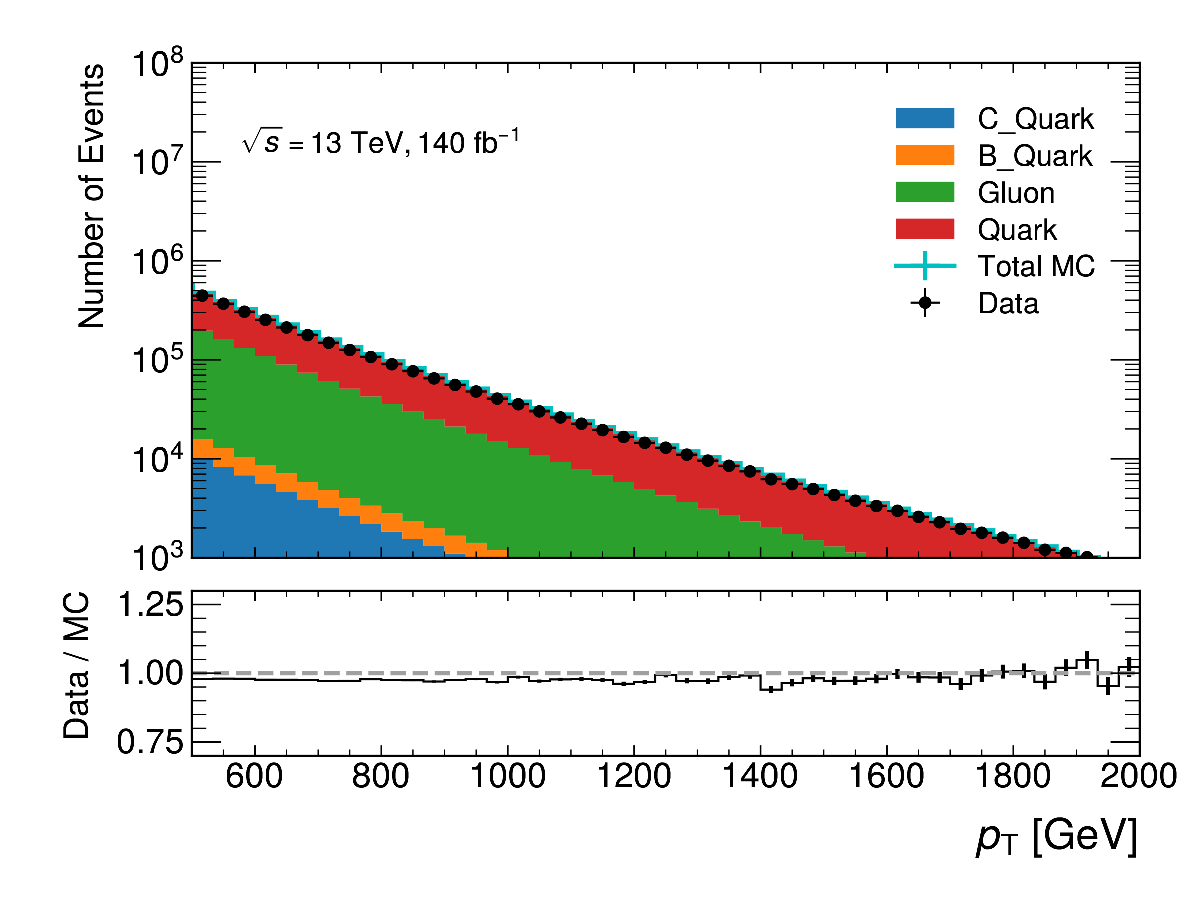
\includegraphics[width=0.48\textwidth]{fig/ADE/Pt_spectrum/none_event_weight/pt_MC16ADE_LeadingJet.pdf}} \quad
        \subfloat[subleading jet  ]{\label{fig:QG-2samplePtaa}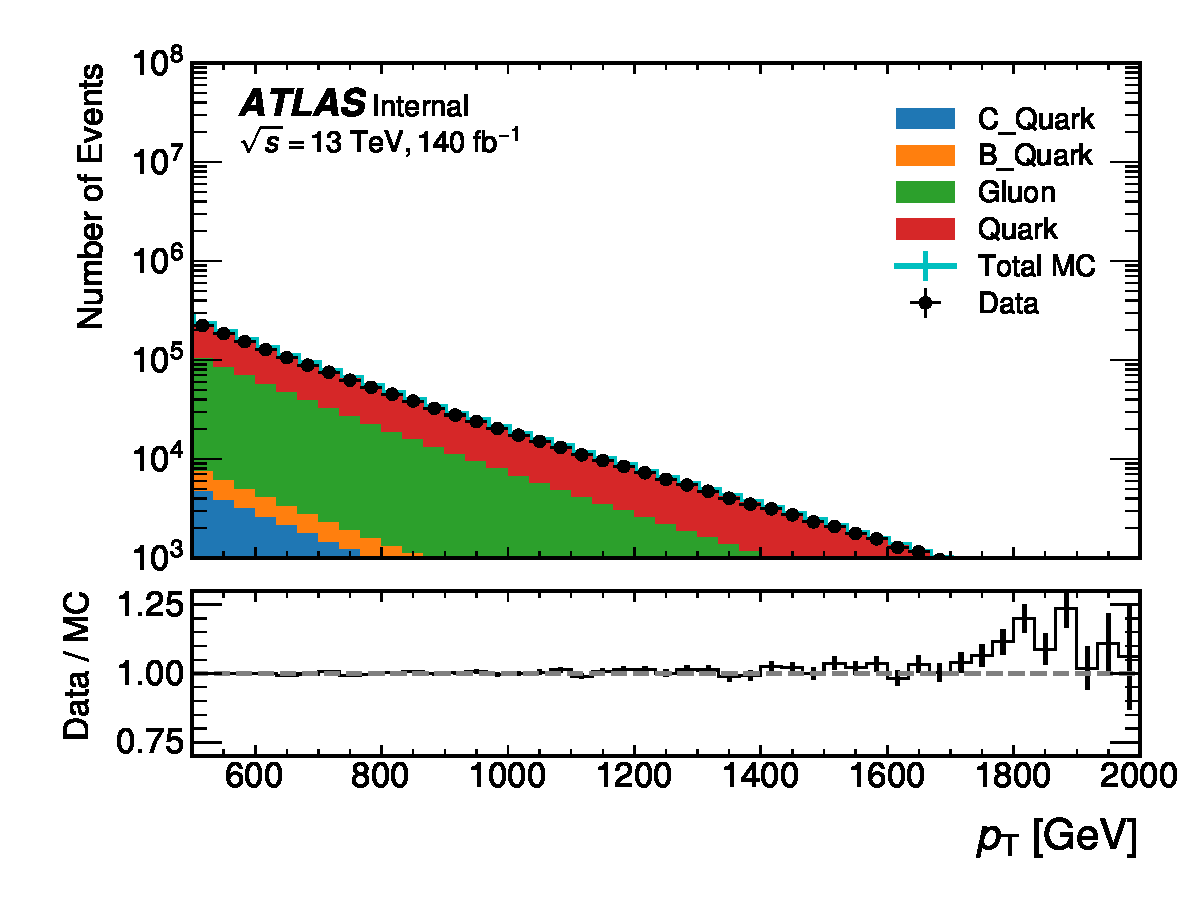
\includegraphics[width=0.48\textwidth]{fig/ADE/Pt_spectrum/none_event_weight/pt_MC16ADE_SubLeadingJet.pdf}} \quad
        \caption[]{
	  The \pt~distribution of the leading jets and sub-leading jets with \pythia samples for dijet event.
                \label{fig:QG-2samplePt}
        }
\end{figure}






\subsection{Quark/gluon tagger construction}
\label{sec:QG-var}
According to QCD, the colour factor of gluons is larger than that of quarks by factor 9/4 ("Casimir ratio")~\cite{ALTARELLI1977298}, which makes gluons emit more particles in the hadronisation than quarks. As a result, a gluon-initiated jet has more charged multiplicity associated and its width is larger than that of a quark-initiated jet. Therefore, the information of the track multiplicity inside a jet is crucial to distinguish quarks from gluons.

The $q/g$ tagging variables used in this study are based on the track multiplicity and are specified as : number of tracks ($\ntrk$), jet width (\wtrk)~\cite{Aad_2014,PhysRevLett.110.212001}, and two point energy correlation function (\cbeta)~\cite{Moult:2016cvt,Larkoski:2013eya} computed from the associated tracks. The expressions are defined as follows:

\begin{description}

  \item[\ntrk] \mbox{} \\
    \ntrk~is a number of tracks associated with the jet. %
    \begin{equation}
    \ntrk = \sum_{\mrm{trk}\in\mrm{jet}}
    \end{equation}

  \item[\wtrk] \mbox{} \\
    \wtrk~is a track-\pt-weighted width of the jet divided by the scalar sum of track transverse momenta. %
    It is defined as %
    \begin{equation}
      \wtrk = \frac{ \sum_{\mrm{trk}\in\mrm{jet}}\pttrk\Delta R_{\mrm{trk,jet}} }{ \sum_{\mrm{trk}\in\mrm{jet}}\pttrk },
    \end{equation}
    where \pttrk~is a \pt~of a charged track reconstructed by the ID and %
    $\Delta R_{\mrm{trk,jet}}$ is a distance in the $\eta-\phi$ plane between the track and the jet axis. %

  \item[\cbeta] \mbox{} \\
    Two point energy correlation function is defined as %
    \begin{equation}
      \cbeta = \frac{ \sum_{i, j\in\mrm{jet}}^{i\neq j} p_{\mrm{T}, i}p_{\mrm{T}, j} \left( \Delta R_{i,j} \right)^{\beta=0.2} }%
        { \left( \sum_{\mrm{trk}\in\mrm{jet}} \pttrk  \right)^{2} }, 
    \end{equation}
    where $i$ and $j$ denote tracks associated with the jet and the sum runs over all the combination of two tracks. % 
    The $\beta$ is fixed to $0.2$, which is known to be suitable for $q/g$ tagging.%~\cite{ref30}. % 

\end{description}

%\FloatBarrier
\subsubsection{The BDT tagger}

Multivariate Analysis (MVA) is a technique introduced to discriminate signal from background, one type of classification algorithm in MVA is the BDT. A tree structure is built to classify datasets through a sequence of branching binary decisions. Data with desirable features is kept by discriminating algorithm whereas others are rejected. Each decision point made construct a node at each level of the decision tree, and a score is assigned to every classifier that goes into the boosting process based on its error rate. One decision node can have two or more branches to split the datasets. Such procedure is iterated from top to down so that a termination condition such as the minimum number of samples in a node or a maximum depth in a tree depth is met. A diagram of a single decision tree is shown in Figure.~\ref{Fig.bdt}. After all series of cuts are applied, the BDT is defined. Therefore, a cut based on the BDT score can be employed as the most correct classification of datasets.

\begin{figure}[htb] 
	\centering  
	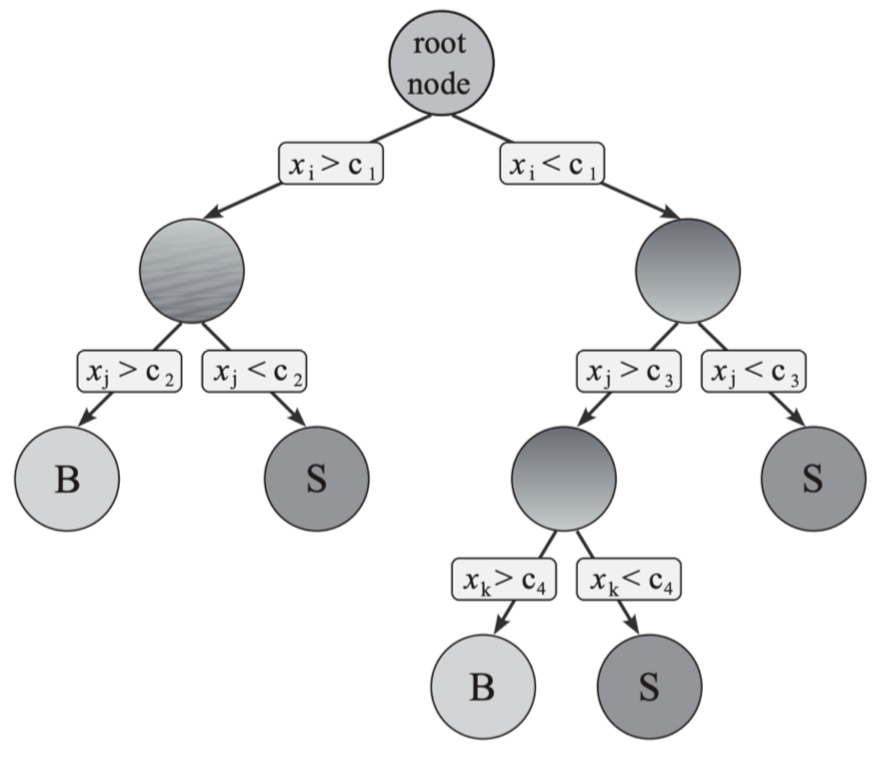
\includegraphics[width=11cm]{./fig/bdt.png}
	\caption{A scheme of a single decision tree with a depth of three}
	\label{Fig.bdt}
\end{figure}

The BDT tagger is constructed by the combination of tracking-related observables: \ntrk, \wtrk, \cbeta~and \pt~of a jet are included as the distribution of the track multiplicity is affected by them. In this study, the BDT score is used to classify quark- or gluon-jets from the multi jet samples, with the truth-labelled information from MC to train until a quark signal efficiency larger than 90\% is reached.


The BDT tagger is trained using the LGBMClassifier from lightGBM~\cite{NIPS2017_6449f44a} framework, and hyper-parameter tuning is performed with Optuna~\cite{akiba2019optuna}. The MC \pythia samples are employed.

An individual score is allocated to each BDT within the boosting procedure, factoring in its error rate.  This BDT score serves as the criterion for classifying a given jet as either a quark-jet or a gluon-jet. 

\paragraph{Feature selections}\mbox{}\par
Drawing upon the features employed during the training process, an exploration of the correlation matrix is undertaken to assess the interdependence among jet attributes, including \pt, \abseta, and jet substructure variables \ntrk, \wtrk, \cbeta, and the BDT. Figure~\ref{fig:weighted_corr} shows \ntrk, \wtrk~and \cbeta exhibit notable interrelationships among themselves, displaying relatively robust correlations. In contrast, \pt~and $\eta$ display a diminished level of correlation. The distributions of all single jet substructure variables and BDT score with systematic uncertainty in forward and central regions are shown in Figure~\ref{fig:QG-pythia-Unc_Ntrk-wp11}. The distributions of all single jet substructure variables and BDT score with systematic uncertainty of quark- and gluon-jets in different \pt~ranges from the MC simulation are shown in Figure~\ref{fig:QG-pythia-Unc_Ntrk-wp11q}.

\begin{figure}[htb]
	\centering
	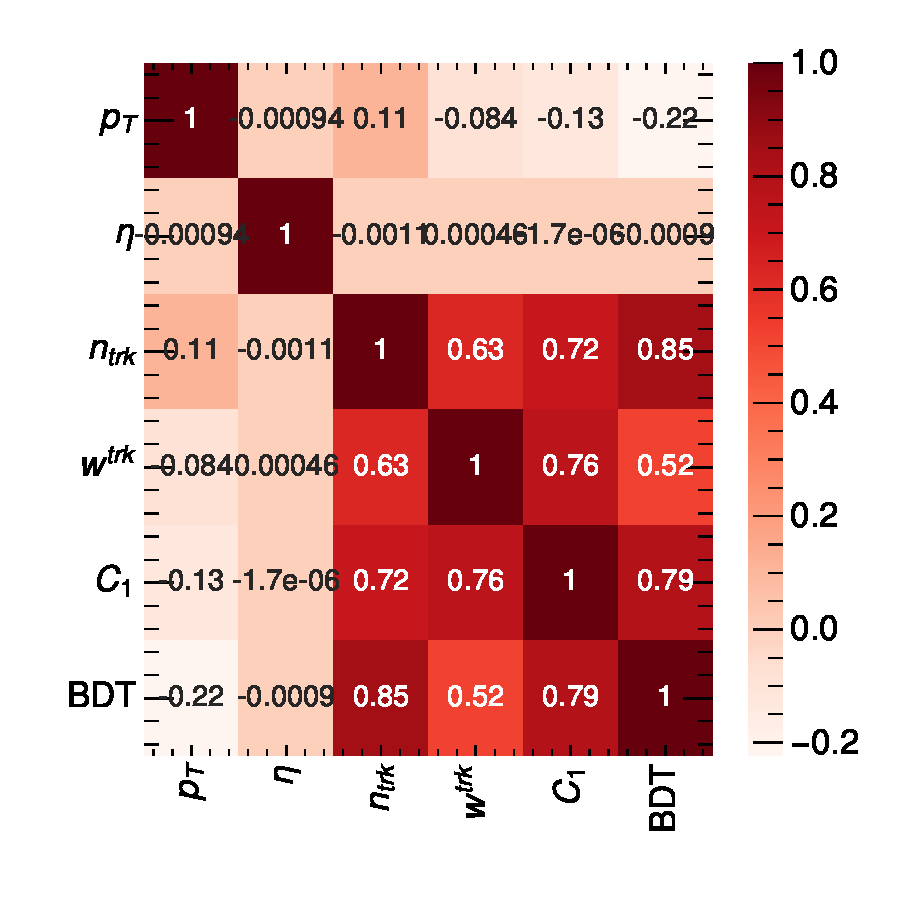
\includegraphics[width=0.65\textwidth]{fig/ADE/new_GBDT/corr.pdf}
	\caption{correlation matrix of jet variables.}
	\label{fig:weighted_corr}
\end{figure}

\begin{figure}[htbp]
	\centering
	\subfloat[]{\label{fig:QG-pythia-UncPythiaQa_Ntrk-wp1}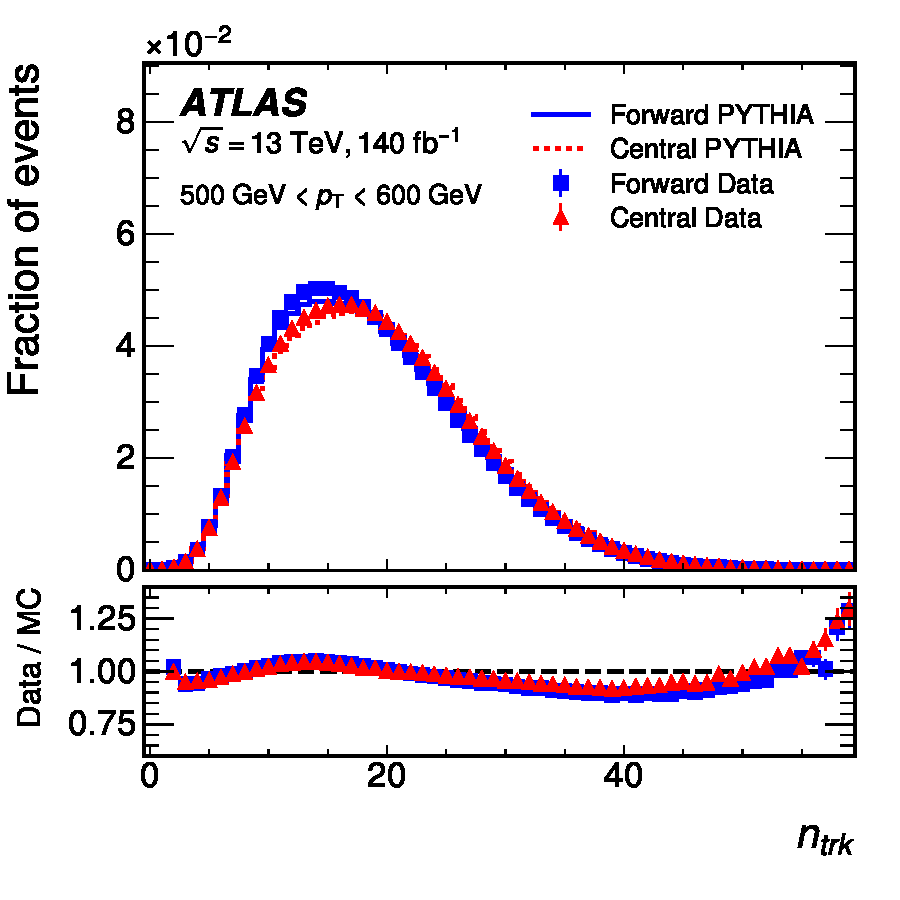
\includegraphics[width=0.45\textwidth]{fig/FvsC_syst/MCvsData_FvsC_500_none_reweight_jet_nTracks.pdf}}\quad
	\subfloat[]{\label{fig:QG-pythia-UncPythiaQb_Ntrk-wp2}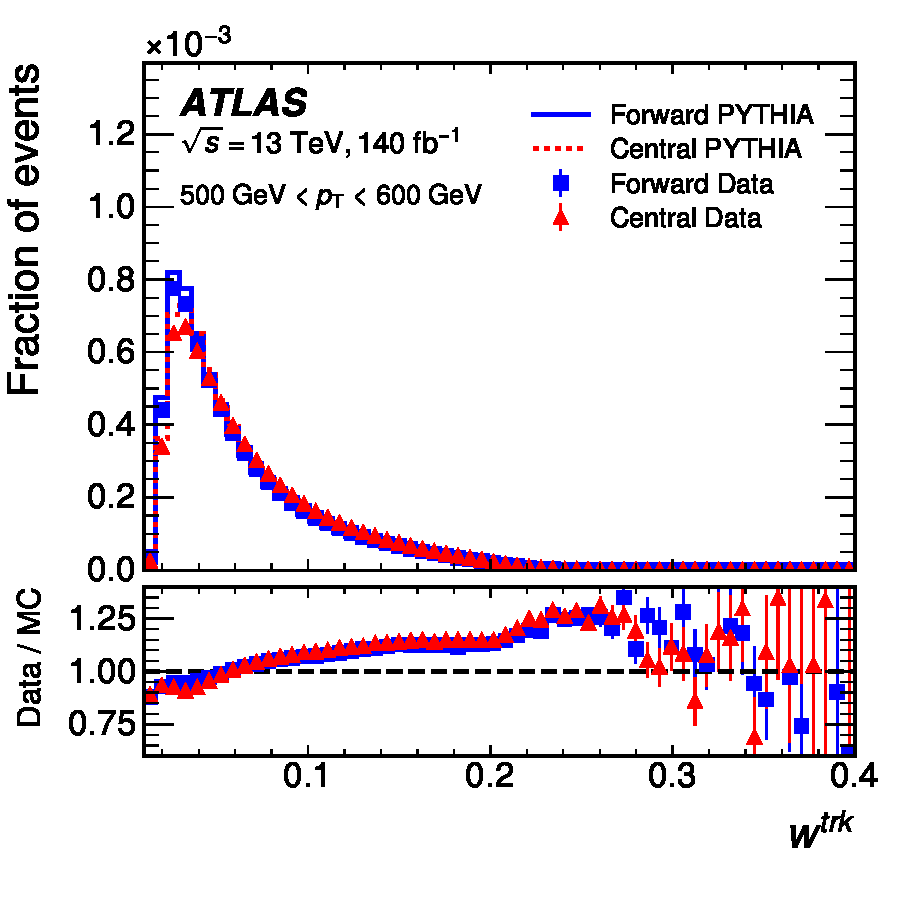
\includegraphics[width=0.45\textwidth]{fig/FvsC_syst/MCvsData_FvsC_500_none_reweight_jet_trackWidth.pdf}}\\
	\subfloat[]{\label{fig:QG-pythia-UncPythiaQa_Ntrk-wp3}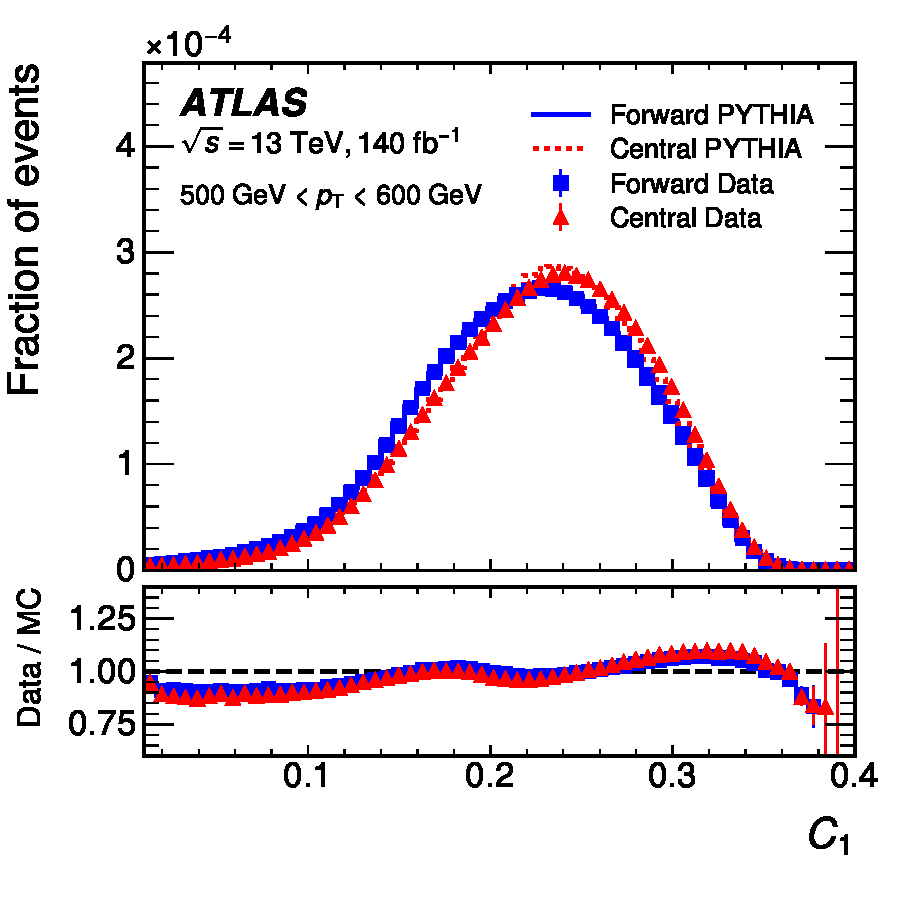
\includegraphics[width=0.45\textwidth]{fig/FvsC_syst/MCvsData_FvsC_500_none_reweight_jet_trackC1.pdf}}\quad
	\subfloat[]{\label{fig:QG-pythia-UncPythiaQb_Ntrk-wp4}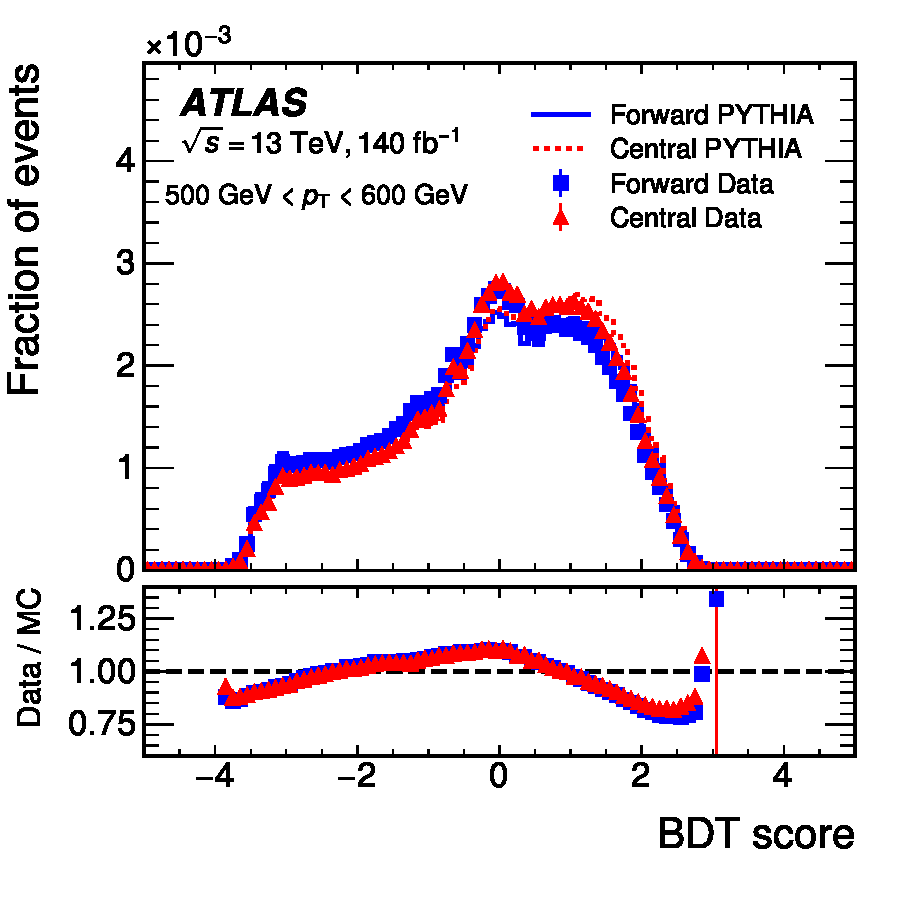
\includegraphics[width=0.45\textwidth]{fig/FvsC_syst/MCvsData_FvsC_500_none_reweight_GBDT_newScore.pdf}}
	\caption[]{
		The distributions of \ntrk~\subref{fig:QG-pythia-UncPythiaQa_Ntrk-wp1}, \wtrk~\subref{fig:QG-pythia-UncPythiaQb_Ntrk-wp2}, $C_1$~\subref{fig:QG-pythia-UncPythiaQa_Ntrk-wp3} and BDT score~\subref{fig:QG-pythia-UncPythiaQb_Ntrk-wp4} in the forward and central regions in data (closed symbols) and the \pythia MC (lines) are shown in the upper panels. The bottom panels show the ratio of the data and the MC. The distributions shown are for jet \pt~in the range between 500 GeV and  600 GeV. The vertical error bars show the statistical uncertainty.
		\label{fig:QG-pythia-Unc_Ntrk-wp11}
	}
\end{figure}


\begin{figure}[htbp]
	\centering
	\subfloat[]{\label{fig:QG-pythia-UncPythiaQa_Ntrk-wp1}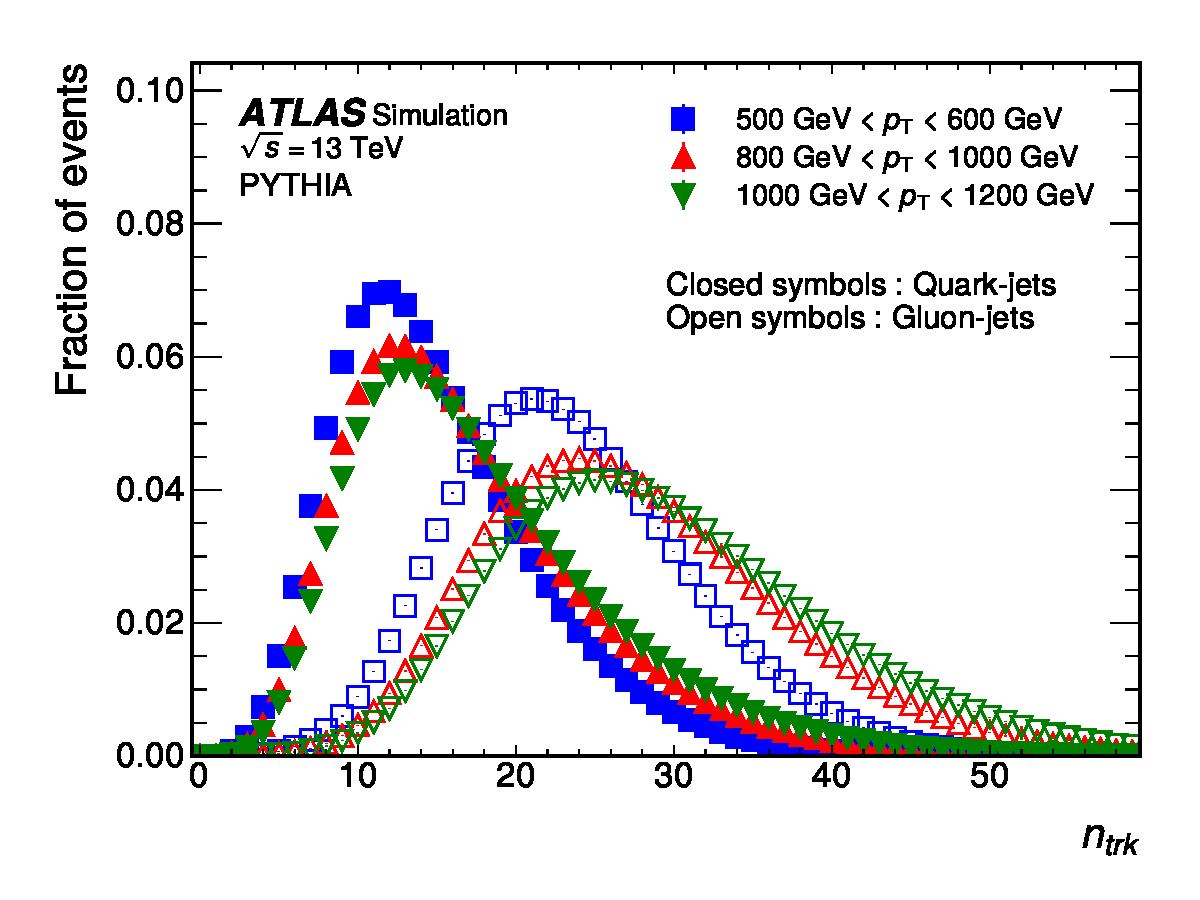
\includegraphics[width=0.45\textwidth]{fig/FvsC_syst/MCvsData_QvsG_1500_none_reweight_jet_nTracks_binned.pdf}}\quad
	\subfloat[]{\label{fig:QG-pythia-UncPythiaQb_Ntrk-wp2}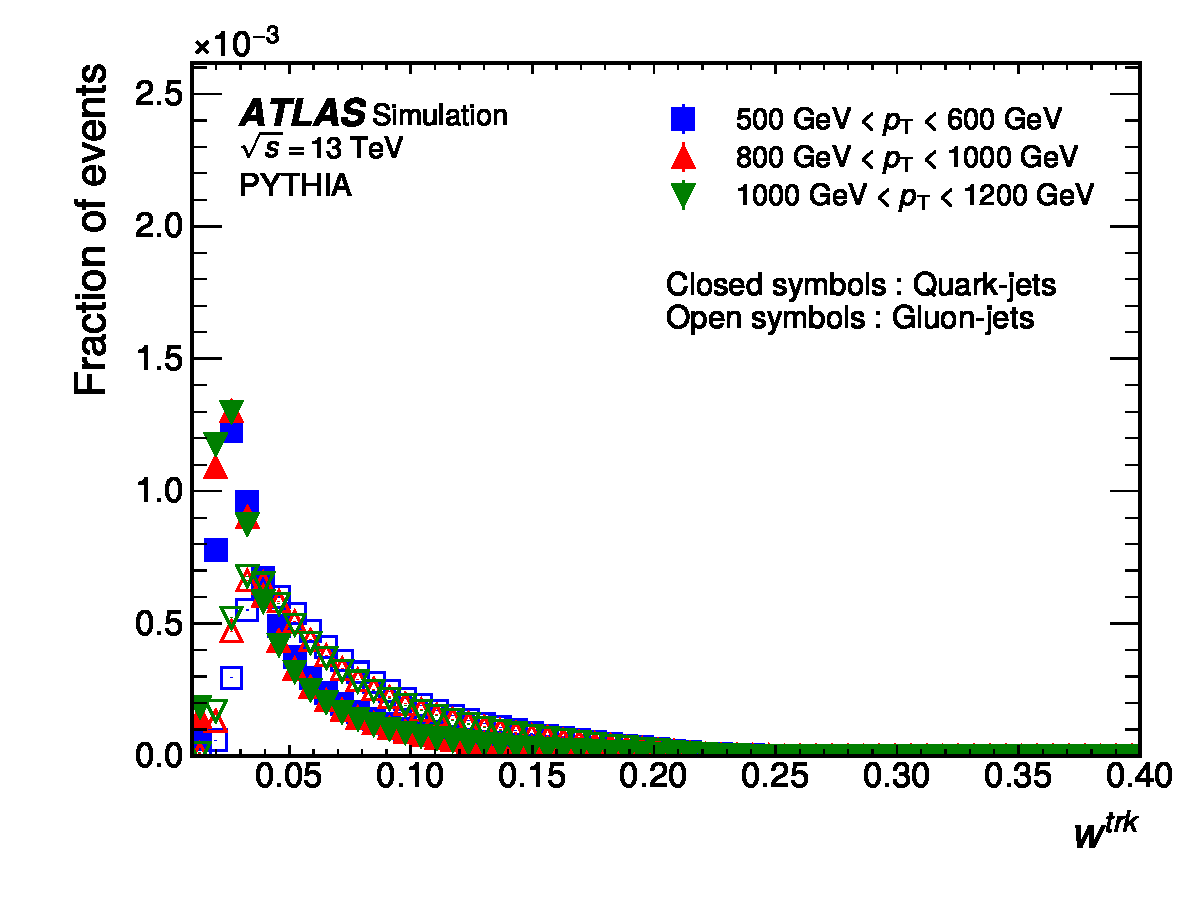
\includegraphics[width=0.45\textwidth]{fig/FvsC_syst/MCvsData_QvsG_1500_none_reweight_jet_trackWidth_binned.pdf}}\\
	\subfloat[]{\label{fig:QG-pythia-UncPythiaQa_Ntrk-wp3}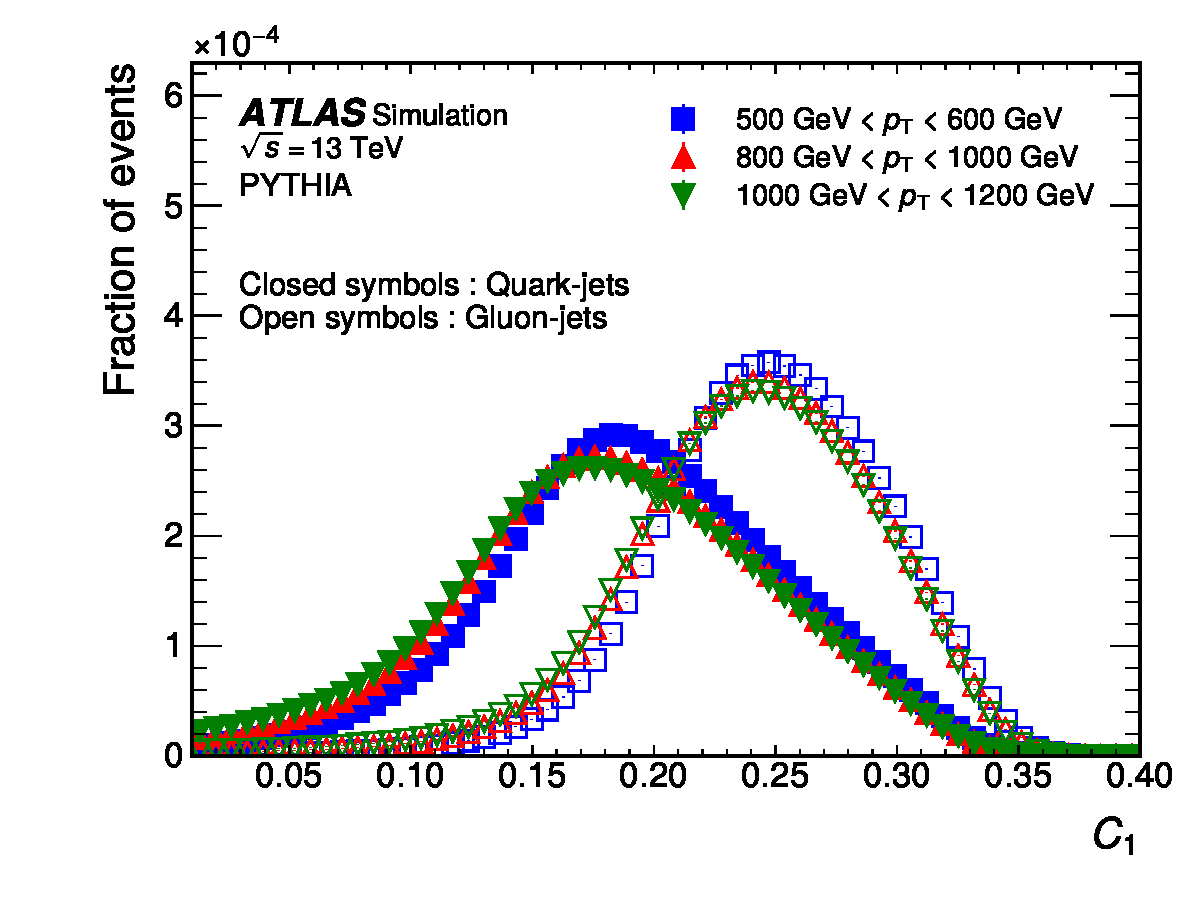
\includegraphics[width=0.45\textwidth]{fig/FvsC_syst/MCvsData_QvsG_1500_none_reweight_jet_trackC1_binned.pdf}}\quad
	\subfloat[]{\label{fig:QG-pythia-UncPythiaQb_Ntrk-wp4}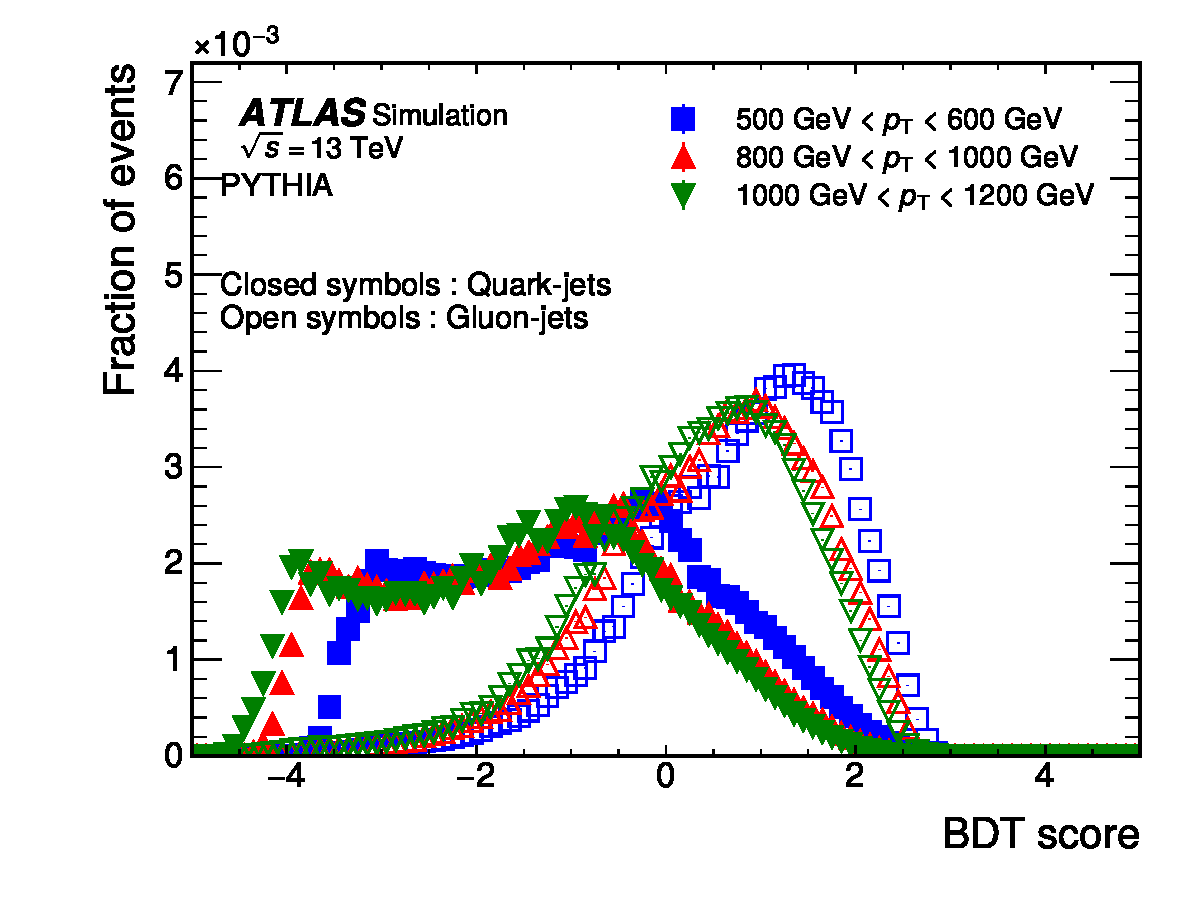
\includegraphics[width=0.45\textwidth]{fig/FvsC_syst/MCvsData_QvsG_1500_none_reweight_GBDT_newScore_binned.pdf}}
	\caption[]{
		The distributions of \ntrk~\subref{fig:QG-pythia-UncPythiaQa_Ntrk-wp1}, \wtrk~\subref{fig:QG-pythia-UncPythiaQb_Ntrk-wp2}, $C_1$~\subref{fig:QG-pythia-UncPythiaQa_Ntrk-wp3} and BDT score~\subref{fig:QG-pythia-UncPythiaQb_Ntrk-wp4} in the quark-jets (closed symbols) and gluon-jets (open symbols) in given \pt~regions using the \pythia MC samples.
		\label{fig:QG-pythia-Unc_Ntrk-wp11q}
	}
\end{figure}

Rather than employing multiple BDTs for different \pt~ranges, an universal BDT can be trained using events in all \pt~ranges.
Given the intrinsic correlation between \ntrk~and the jet \pt, a natural way to choose features is including \pt~in addition to three $q/g$ tagging variables.    
Concerning the remaining variable, $\eta$, two comparative scenarios are juxtaposed: one involves its inclusion, and the other pertains to its exclusion. This comparison facilitates an assessment of whether or not to incorporate \abseta.

\begin{enumerate}
	\item \pt, \ntrk, \wtrk~and \cbeta
	\item \pt, \abseta, \ntrk, \wtrk~and \cbeta
\end{enumerate}

The result depicted in Figure~\ref{fig:QG-training_scenario_compare_500_600} shows a distinct discrepancy when \abseta is encompassed within the training. 
This violates the assumptions that the partons distribution in more forward and more central regions should not change. Specifically, the distribution of BDT scores for forward quarks substantially diverges from that of central quarks, a trend that is similarly observed for gluons. Moreover, adopting the BDT tagger that incorporates \abseta~would result in inadequate performance for jets situated within the central region when this tagger is applied to a pure sample of quark-jets (e.g., $Z$+jet samples).
In the present analysis, the BDT is endowed with the spectra of \pt, \ntrk, \wtrk, and \cbeta, as exemplified in scenario 1. 
At detector-level, however, the observed radiation pattern within jets no longer remains unaffected by \abseta, owing to variances in the detector material and technology. To counteract this effect, a subsequent re-weighting procedure is implemented, described in Section~\ref{sec:QG-closure}. 

\begin{figure}[htb]
	\centering
	\subfloat[Training without \abseta, scenario 1 ]{\label{fig:QG-training-wo-eta-500}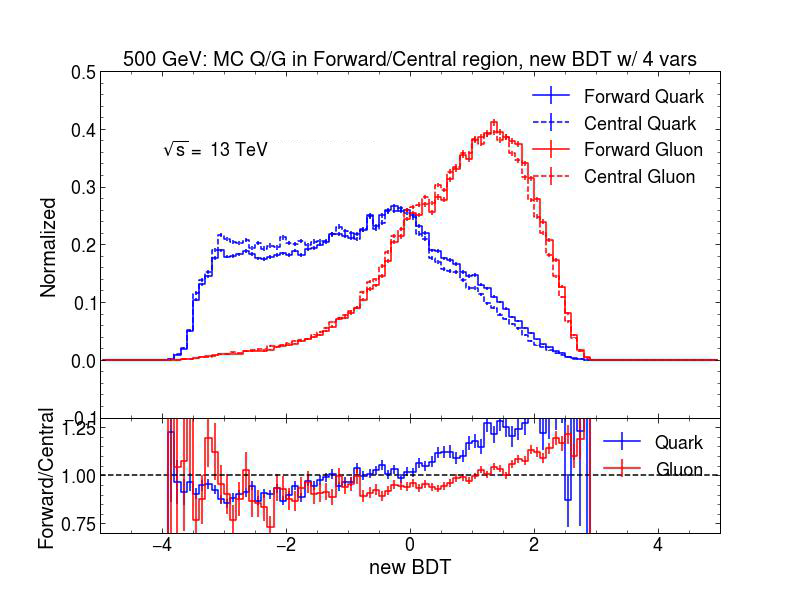
\includegraphics[width=0.45\textwidth]{fig/ADE/new_GBDT/4vars_plots/MC_truth_Q_G_FvsC_500_GBDT_newScore_None.jpg}} \quad
	\subfloat[Training with \abseta, scenario 2]{\label{fig:QG-training-w-eta-500}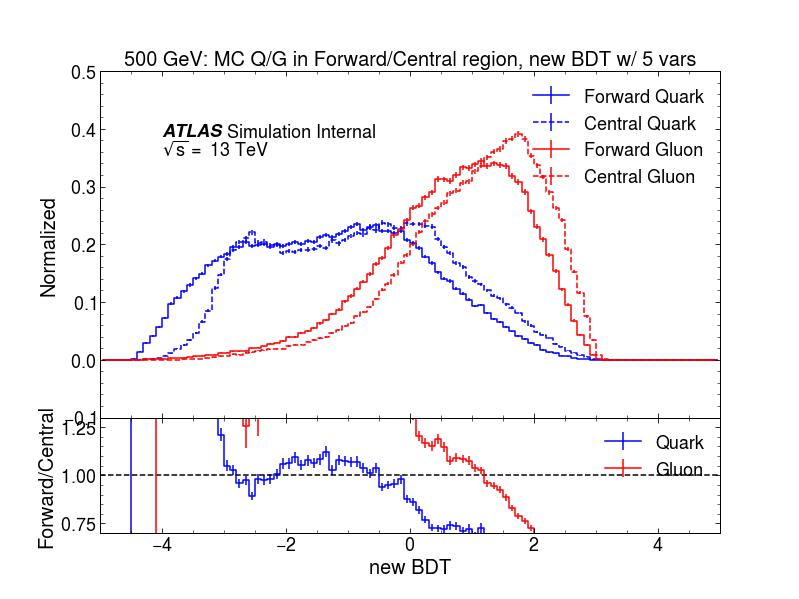
\includegraphics[width=0.45\textwidth]{fig/ADE/new_GBDT/5vars_abseta_plots/MC_truth_Q_G_FvsC_500_GBDT_newScore_None.jpg}}
	\caption[]{
		The comparison of BDT distribution for different scenarios in the jet \pt~range from 500 to 600 GeV. %.
		\label{fig:QG-training_scenario_compare_500_600}
	}
\end{figure}

\paragraph{Training weights}\mbox{}\par
An additional data processing step is conducted to modify the event weights, such that a flat distribution of the \pt~spectrum is given. 
This adjustment is motivated by the observation that higher \pt~jets have less probability to occur, so the training on the higher \pt~jets need to be emphasise. This newly introduced weight, referred to as the "flat \pt-weight" within this context, is exclusively employed during the training process. Conversely, for other scenarios, such as assessing tagger performance on validation datasets and subsequent calibration endeavours, the original event weights based on physical considerations remain employed.

\begin{figure}[htb]
	\centering
	\subfloat[Physical event weight]{\label{fig:QG-training-pt-event-weight}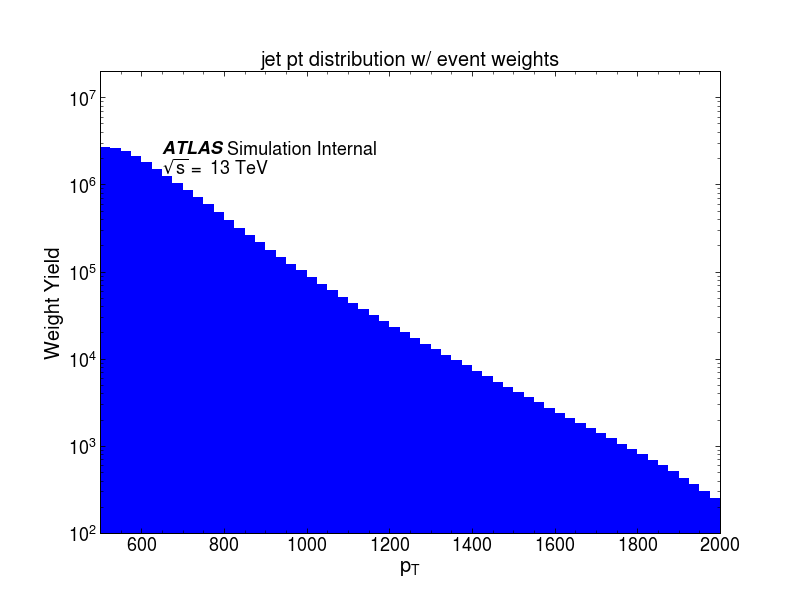
\includegraphics[width=0.45\textwidth]{fig/ADE/new_GBDT/pt_event_weight.png}} \quad
	\subfloat[Flat \pt-weight]{\label{fig:QG-training-pt-flatpt-weight}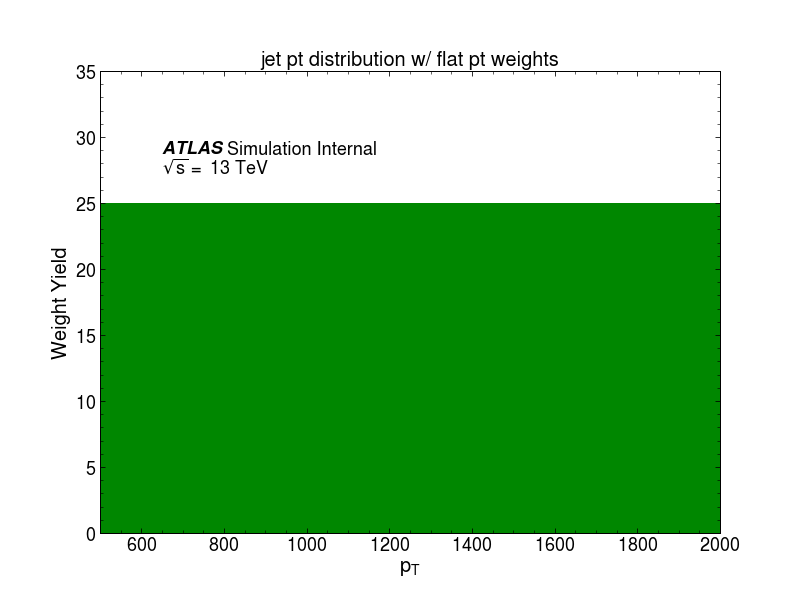
\includegraphics[width=0.45\textwidth]{fig/ADE/new_GBDT/pt_flatpt_weight.png}}
	\caption[]{
		The comparison of jet \pt~distributions with different weights. %.
		\label{fig:QG-training-pt-weight-compare}
	}
\end{figure}

\paragraph{Training Configuration}\mbox{}\par

Approximately 30\% of the data from each period of the MC \pythia8 A, D, E is randomly allocated for the training investigation, constituting an aggregate of roughly 60 million jets. 
The dataset division for training, validation, and testing is structured in a ratio of 80\% for training, 10\% for validation, and 10\% for testing.

Optuna is employed to conduct a search for optimal hyperparameters. Following the hyperparameter tuning process, the most optimal model is achieved after 100 iterations of such procedure. The optimised parameters are listed:

\begin{itemize}
	\item bagging\textunderscore fraction 0.9176347488279626
	\item bagging\textunderscore freq 2
	\item feature\textunderscore fraction 0.9084973008559477
	\item lambda\textunderscore l1 0.0016400096502256838
	\item lambda\textunderscore l0.006327330258011633
	\item min\textunderscore child\textunderscore samples 13
	\item num\textunderscore leaves 224
\end{itemize}

The performance of a classification model at all classification criteria can be illustrated using a receiver operating characteristic (ROC) curve. The idea is to compare the true positive rate (TPR, also known as sensitivity, recall or probability of detection) against the false positive rate (FPR, also known as the probability of false alarm) at different criteria given. Consider a binary classification case, where the outputs are either labelled as positive (p) or negative (n), in total there are four possible outputs from a two-class prediction problem. A true positive (TP) is given if the output from a prediction is p and the actual value is also p, otherwise a false positive (FP) is assigned if the actual value is n. Conversely, a true negative (TN) is given if both the prediction outcome and the actual value are n, whereas a a false negative (FN) is assigned if the actual value is p. TPR as a synonym for recall is defined as:
\begin{equation}
	TPR = TP/(TP+FN)
\end{equation}
while the FPR is defined as: 
\begin{equation}
	FPR = FP/(FP+TN)
\end{equation}

In this analysis, the prediction true is defined by higher \abseta jet and prediction negative is defined by lower \abseta jet. The actual truth value is given by the quark jet from the MC truth information, whereas the actual negative value is given by the gluon truth information. Thus the quark efficiency is the TPR and the gluon rejection is FPR. An Area Under the ROC Curve (AUC) is used to evaluate the performance of a classifier, the better performance is indicated by higher AUC values.

Several ROC plots are made to compare different features and the BDT in different \pt~ranges. 
To check whether the BDT tagger is overtrained, the shape comparison is shown in Figure~\ref{fig:overtraining-validation}, between training dataset and validation dataset.  
No overtraining is observed as the distribution of training dataset is very similar to that of testing dataset. 

Figure~\ref{fig:QG-ROC_500_600} shows the ROC curve for all single jet variables and the BDT-tagger in given \pt~ranges in forward and central regions. Figure~\ref{fig:QG-ROC_800_1000}  shows the AUC of both \ntrk-only tagger and the BDT-tagger as a function of jet \pt. 
\begin{figure}[h]
	\centering
	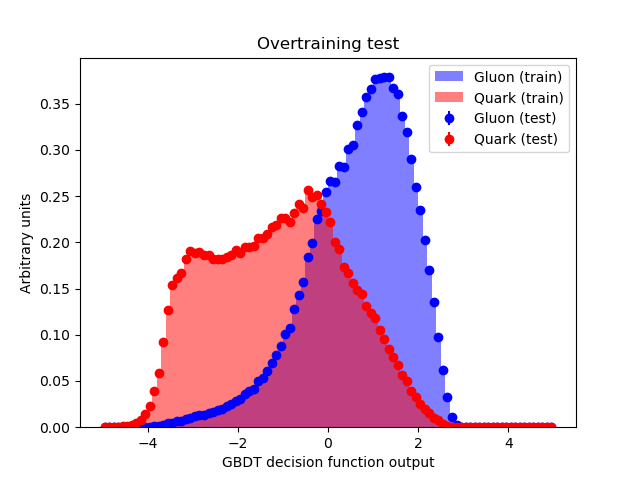
\includegraphics[width=0.65\textwidth]{fig/ADE/new_GBDT/4vars_plots/overtrain_validation.png}
	\caption{Overtraining validation}
	\label{fig:overtraining-validation}
\end{figure}

\begin{figure}[htb]
	\centering
	\subfloat[Forward region ]{\label{fig:QG-NtrkDataMCinclPythiaa}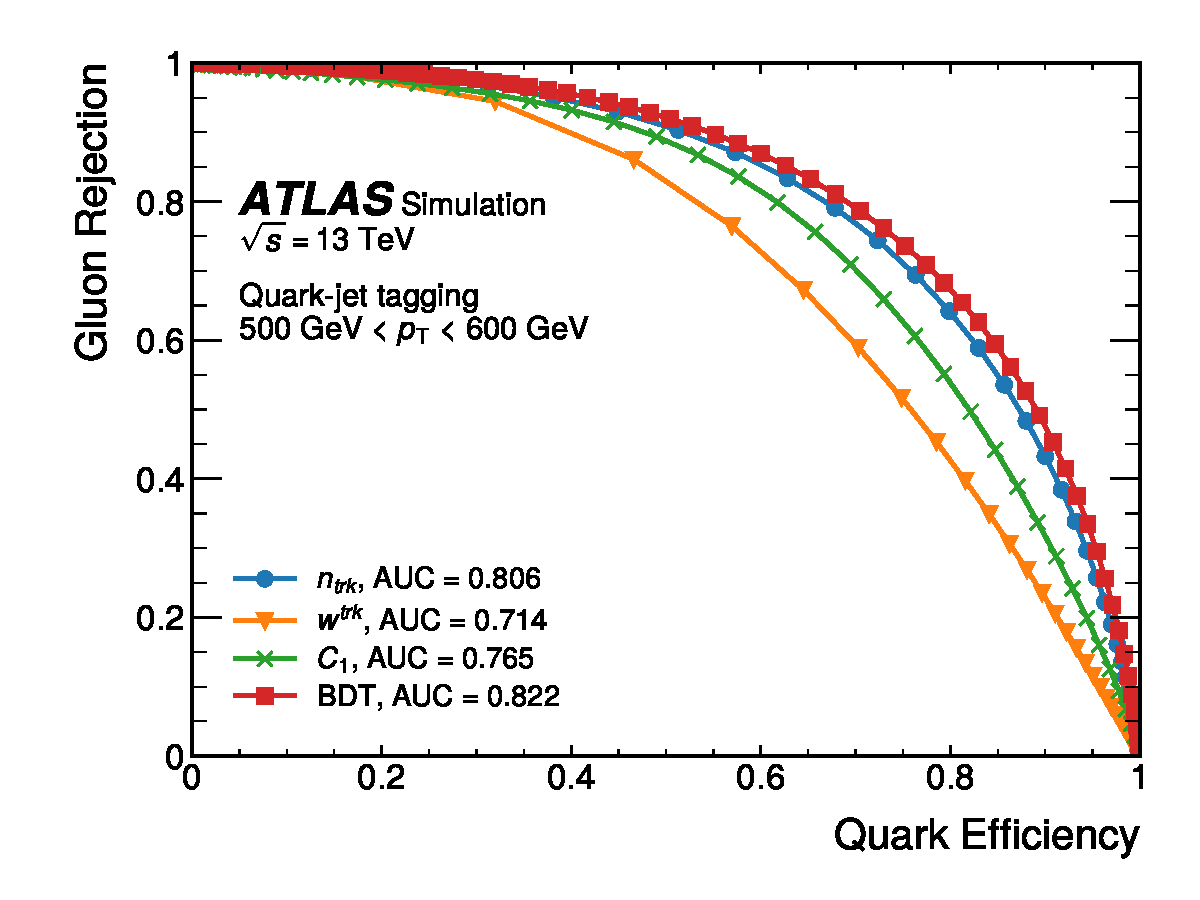
\includegraphics[width=0.48\textwidth]{fig/ROC/ROC_500_Forward_none.pdf}} \quad
	\subfloat[Central region ]{\label{fig:QG-NtrkDataMCinclPythiab}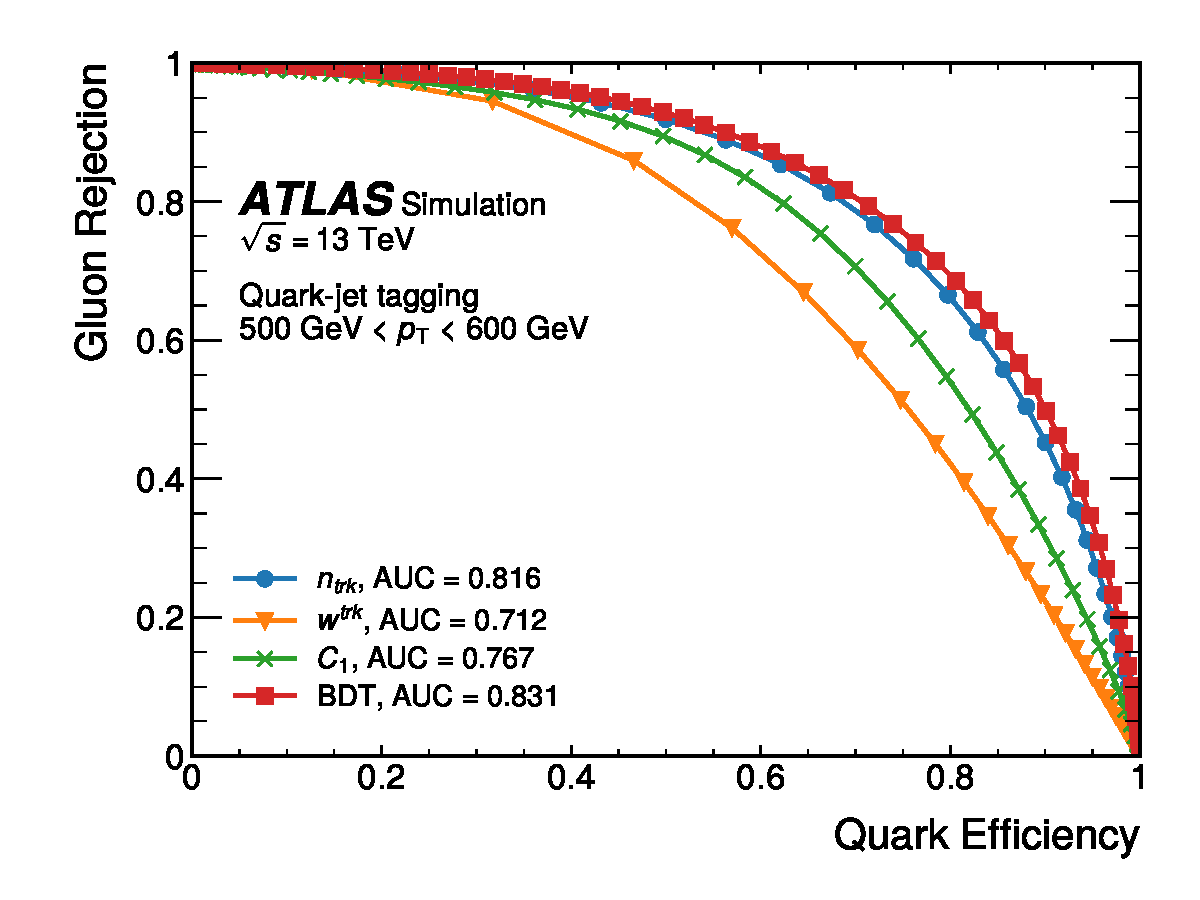
\includegraphics[width=0.48\textwidth]{fig/ROC/ROC_500_Central_none.pdf}}
	\caption[]{
		The ROC Curve for different taggers in the given jet \pt. %.
		\label{fig:QG-ROC_500_600}
	}
\end{figure}


\begin{figure}[htb]
	\centering
	\subfloat[Forward region ]{\label{fig:QG-NtrkDataMCinclPythiaa}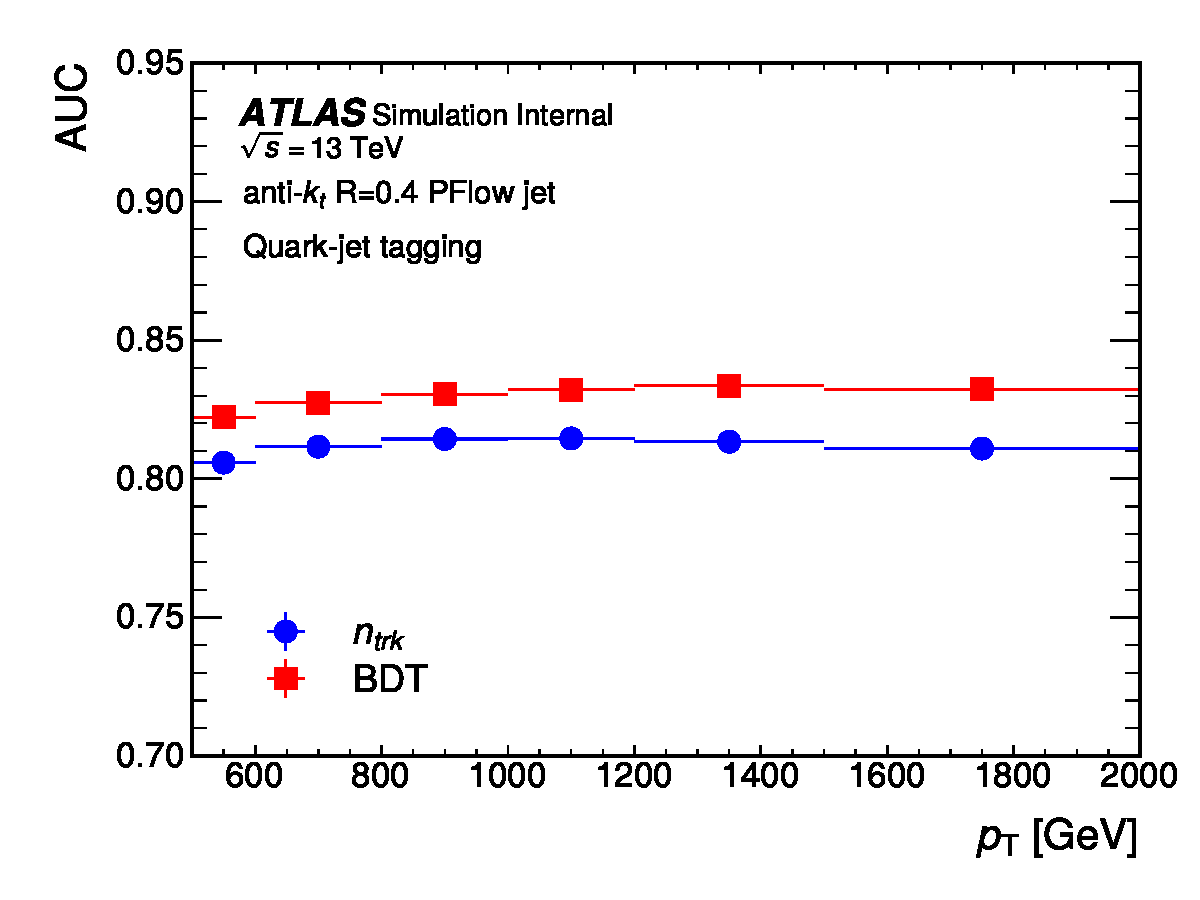
\includegraphics[width=0.48\textwidth]{fig/ROC/pt_Forward_GBDT_newScore.pdf}} \quad
	\subfloat[Central region]{\label{fig:QG-NtrkDataMCinclPythiab}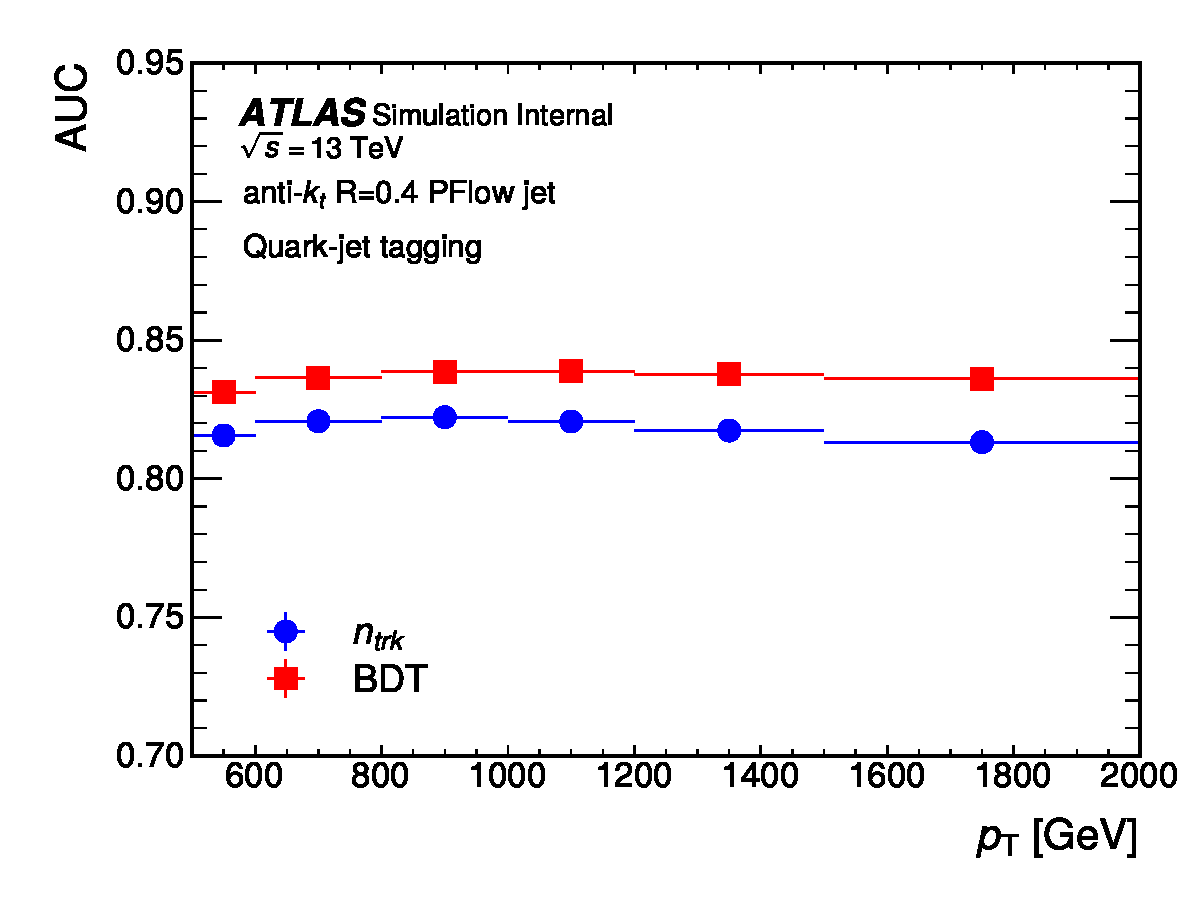
\includegraphics[width=0.48\textwidth]{fig/ROC/pt_Central_GBDT_newScore.pdf}}
	\caption[]{
		The AUC for different taggers across jet \pt. %.
		\label{fig:QG-ROC_800_1000}
	}
\end{figure}

%A receiver operating characteristic (ROC) curve,  is a graph showing the performance of a classification model at all classification thresholds. The ROC curve is created by plotting the true positive rate (TPR) against the false positive rate (FPR) at various threshold settings. The true-positive rate is also known as sensitivity, recall or probability of detection. The false-positive rate is also known as the probability of false alarm and can be calculated as (1-specificity).
%
%Consider a two-class prediction problem (binary classification), in which the outcomes are labeled either as positive (p) or negative (n). There are four possible outcomes from a binary classifier. If the outcome from a prediction is p and the actual value is also p, then it is called a true positive (TP); however, if the actual value is n then it is said to be a false positive (FP). Conversely, a true negative (TN) has occurred when both the prediction outcome and the actual value are n, and a false negative (FN) is when the prediction outcome is n while the actual value is p.
%
%TPR is a synonym for recall and is therefore defined as follows: TPR $=$ TP/(TP+FN), while the FPR is defined as follows: FPR $=$ FP/(FP+TN). In this analysis,  \abseta jet is defined as the prediction true and central \abseta jet is defined as the prediction negative, the truth quark-jet from MC simulation is defined as the actual truth value, the gluon-jet is defined as the actual negative value. Thus, the TPR is quark efficiency and FPR is gluon rejection.

%In classification problems, Area Under the ROC Curve(AUC) is used to evluate the classifier performance. The forward AUC values indicate better performance. The AUC are shown in the ROC plots along the legends. 

The \ntrk-only tagger is found to be the most sensitive observable than other individual jet substructure variables for $q/g$ tagging, 
\wtrk~and \cbeta~are less sensitive to the number of tracks inefficiencies because they are defined as ratios, the BDT-tagger which include the $\wtrk$ and $\cbeta$ has better AUC than \ntrk-only tagger across all jet \pt~ranges. This indicates that the BDT-based tagging mechanism has a heightened capacity to discriminate against gluon-jets at the same level of efficiency in identifying quark-jets with \ntrk-only tagger . Both taggers are calibrated in this paper, more details are presented in the next section.

%\wtrk and \cbeta are less sensitive to the number of trackstrack inefficiencies because they are defined as ratios. %only and it has only a small \eta dependency. %
%\texttt{TightPrimary} identified tracks have few fake tracks and only a small \eta dependency. %

%since such a jet substructure information is not used in the conventional SUSY searches and %
%the mis-modeling of the simulation, especially in a gluon, is known in the previous study for q/g tagging in Run1~\cite{QGRun1}. %

\FloatBarrier



\subsection{Matrix Method}
\label{sec:QG-method}
The distribution of q/g tagging variables depend strongly on jet \pt. Thus a matrix method~\cite{ATL-PHYS-PUB-2017-009} approach used to extract the shape of the $q/g$ tagging variables is performed on each \pt~bin defined in Table~\ref{tab:QG-ptbinning} for quark- and gluon-jets, separately. 

\begin{table}[hptb]
\centering
\begin{tabular}{|c|c|c|c|c|c|}
 \hline
 \multicolumn{6}{|c|}{\pt~bin boundary [GeV] } \\ \hline
   500-600 & 600-800 & 800-1000 & 1000-1200 & 1200-1500 & 1500-2000  \\ \hline
  \multicolumn{6}{|c|}{\multirow{2}{*}{Forward \& Central \abseta jet samples in multi-jet}} \\ 
  \multicolumn{6}{|c|}{} \\ \hline
\end{tabular}
\caption{
	The \pt~range division for the calibration of the $q/g$ tagging variables and samples used in extraction of pure quark and gluon jets. %
}
\label{tab:QG-ptbinning}
\end{table}

To measure the performance of the $q/g$ taggers under study, samples exclusively composed of either quark-jets or gluon-jets are needed. In order to deduce the distribution shapes of the $q/g$ tagging variables pertaining to quark- and gluon-jets within the empirical data, a methodology that capitalizes on samples possessing varying q/g ratios is employed. This approach, known as the matrix method~\cite{ATL-PHYS-PUB-2017-009}, facilitates the extraction of the distinct distributions of $q/g$ tagging variables for the aforementioned jet categories.

Pure quark- or gluon-jets can be extracted from forward and central jet samples following the matrix: 
\begin{eqnarray}
	\label{eq:QG-matrix2}
	\left(\begin{array}{c} 
		p_{\mrm{F}}(x)\\ 
		p_{\mrm{C}}(x)\\ 
	\end{array}\right)
	&=&
	\underbrace{
		\left(\begin{array}{cc}
			f_{\mrm{F,Q}}&f_{\mrm{F,G}}\\
			f_{\mrm{C,Q}}&f_{\mrm{C,G}}\\
		\end{array}\right)
	}_{\scalebox{1}{$\equiv F$}}
	\left(\begin{array}{c} 
		p_\mrm{Q}(x)\\ 
		p_\mrm{G}(x)\\ 
	\end{array}\right)
	\\
	\label{eq:QG-invmatrix2}
	%\Leftrightarrow
	\left(\begin{array}{c} 
		p_\mrm{Q}(x)\\ 
		p_\mrm{G}(x)\\ 
	\end{array}\right)
	&=& F^{-1}
	\left(\begin{array}{c} 
		p_{\mrm{F}}(x)\\ 
		p_{\mrm{C}}(x)\\ 
	\end{array}\right).
\end{eqnarray}


where $p_{\mrm{Q,G}}(x)$ represents the distributions of the $q/g$ tagging variable $x$ in pure quark- and gluon-enriched jet samples, 
$p_{\mrm{F}}(x)$ and $p_{\mrm{C}}(x)$ show the distributions of jet variables in forward and central regions, respectively, $f_{\mrm{F/C},\mrm{Q/G}}$ are the fractions of quarks and gluons in a forward or central region. %
The inverse matrix of $F$ is thus constructed and used to extract pure quark/gluon~$p_{\mrm{Q,G}}$. %
Data is used to obtain the distributions of the quark- and gluon-enriched samples, MC is used to calculate the fraction of quarks and gluons in them as shown in Figure~\ref{fig:QG-Fmc}, as well as the distributions of $q/g$ tagging variables. %
The matrix is calculated in each $x$ bin and each jet \pt~range.


\begin{figure}[htb]
	\centering
	\subfloat[]{\label{fig:QG-Fmcd}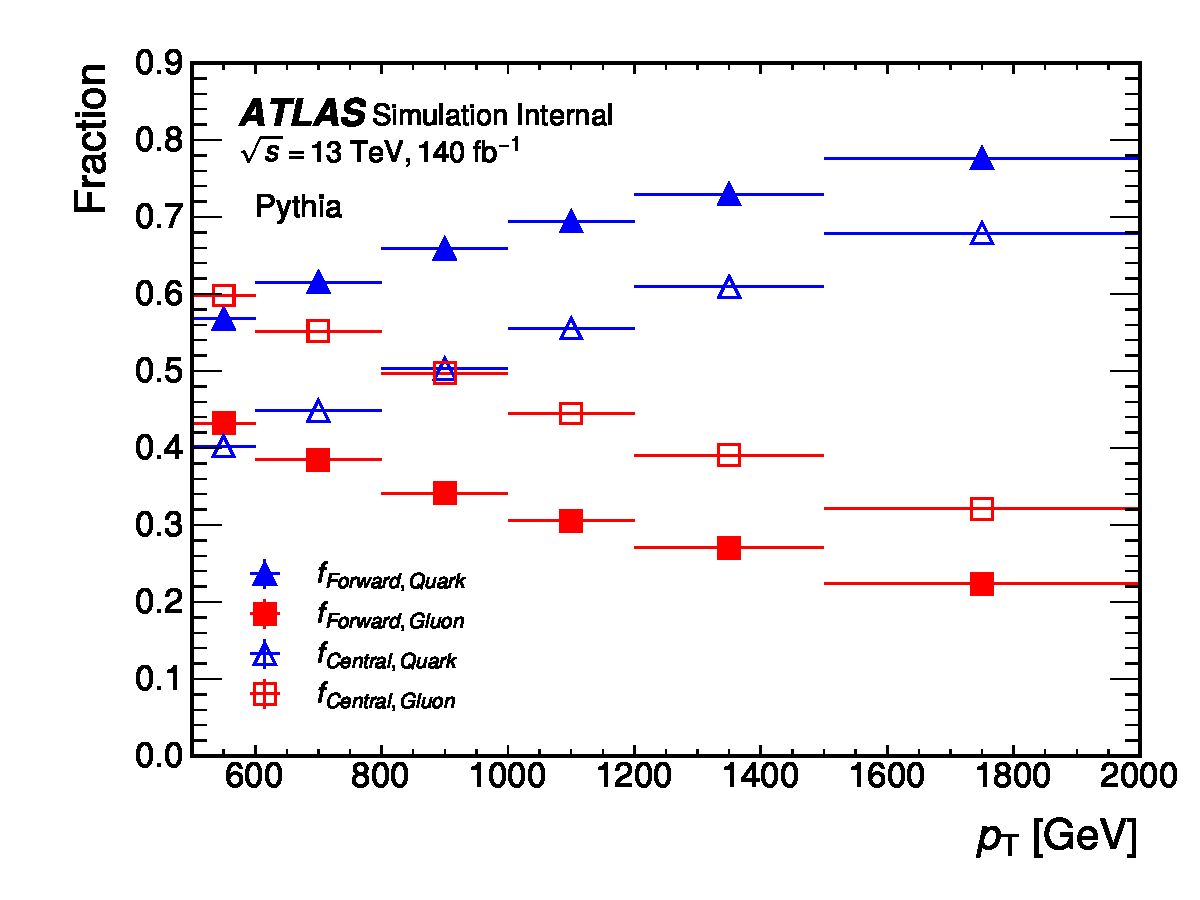
\includegraphics[width=0.6\textwidth]{fig/ADE/frac/Fraction_jet_nTracks_pythia.pdf}}\quad
	\caption[]{
		Fractions of quark-jets and gluon-jets  %
		in forward jet and central jet regions from {\pythia} dijet process. These values are used as elements in $F$ matrix in Equation \ref{eq:QG-matrix2}. %
		\label{fig:QG-Fmc}
	}
\end{figure}

\begin{figure}[htb]
	\centering
	\subfloat[Forward region ]{\label{fig:QG-Quark-Fraction-forward}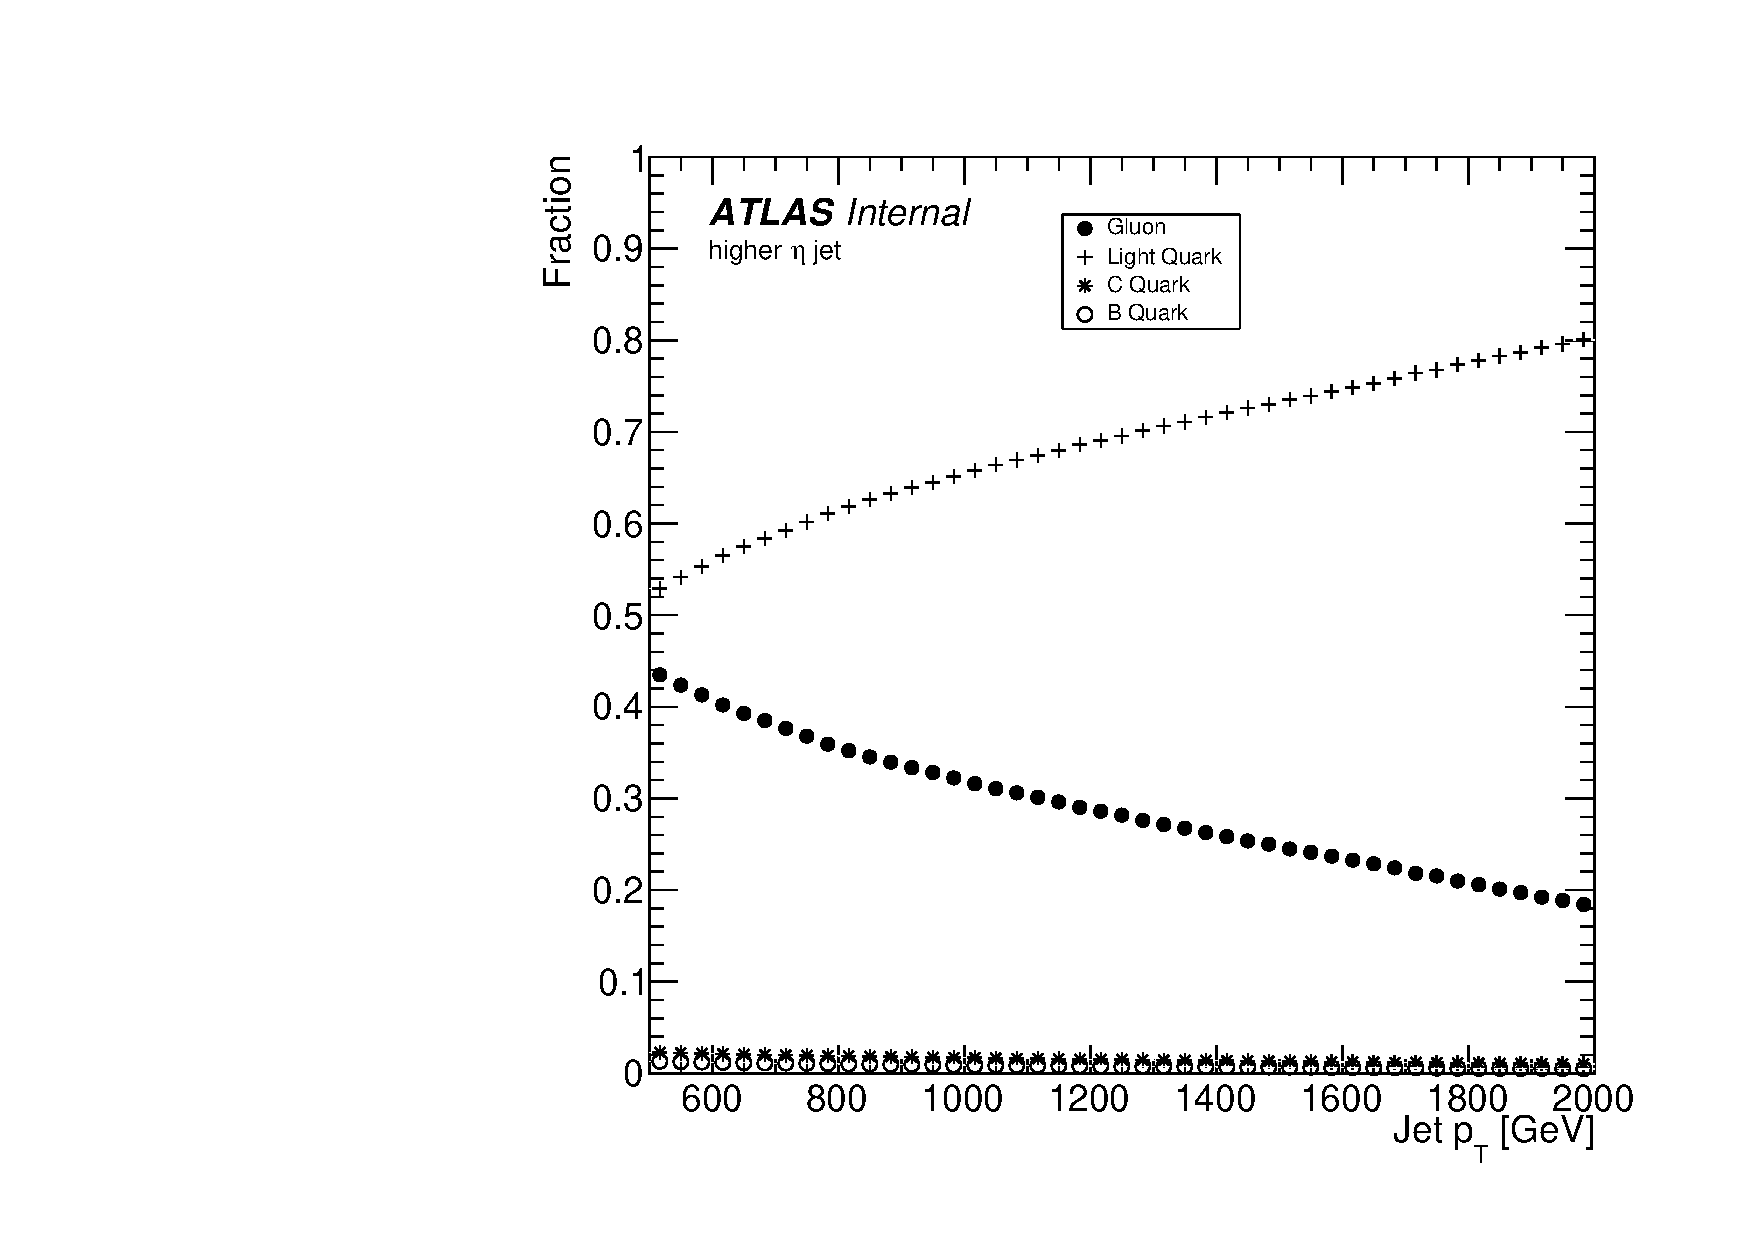
\includegraphics[width=0.45\textwidth]{fig/ADE/higher_fraction.pdf}} \quad
	\subfloat[Central region ]{\label{fig:QG-Quark-Fraction-central}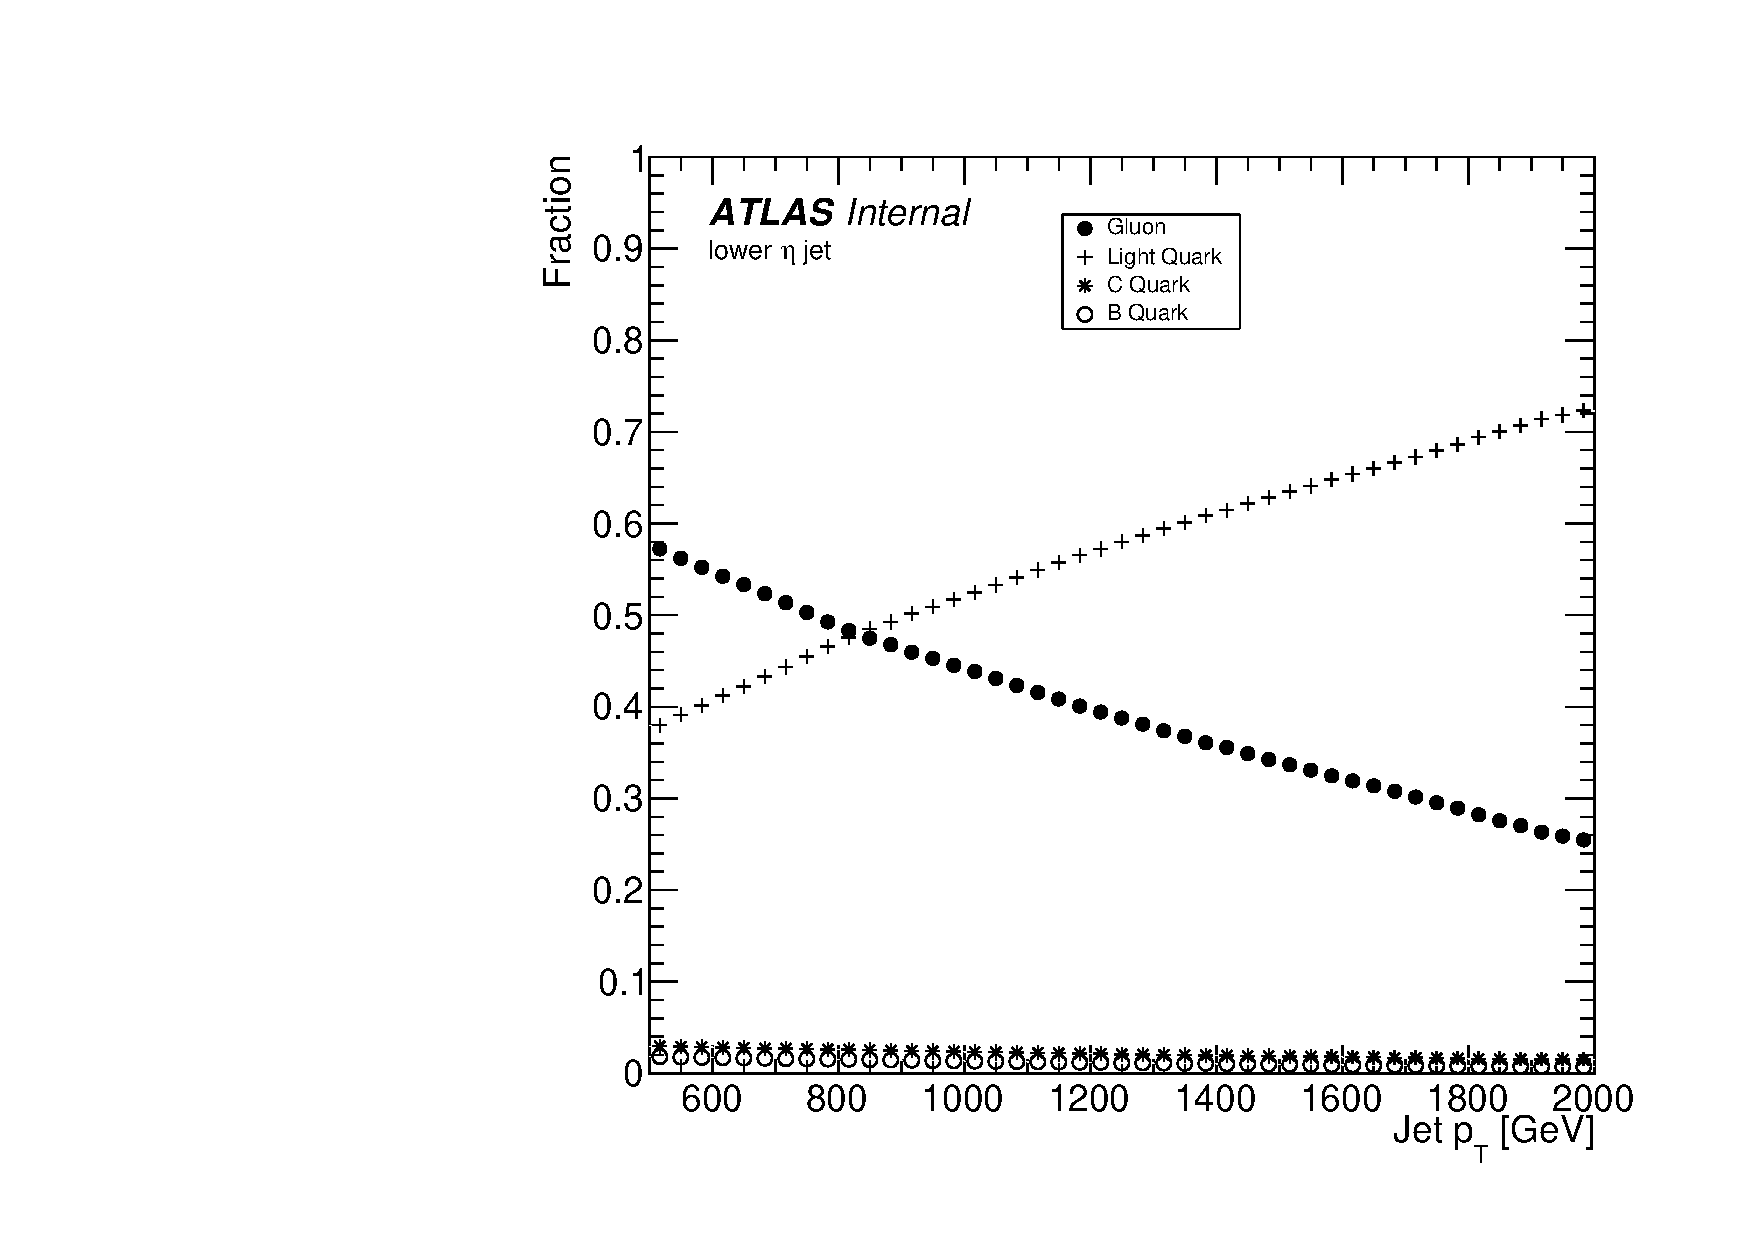
\includegraphics[width=0.45\textwidth]{fig/ADE/lower_fraction.pdf}} \quad
	\caption[]{
		Flavor composition of of forward \subref{fig:QG-Quark-Fraction-forward}  or central  \subref{fig:QG-Quark-Fraction-central} multi-jet events. %.
		\label{fig:QG-quark-fraction}
	}
\end{figure}


Figure~\ref{fig:QG-quark-fraction} illustrates the fraction of light and heavy quark- and gluon-jets in the \pythia8 dijet sample. These fractions are depicted in a stacked format, summing up to a cumulative value of 1. It should be noted that the involvement of heavy flavour quarks constitutes a minor fraction, amounting to a few percent, and is deemed negligible for the later study.
Previous investigations~\cite{ref21} have established that any discrepancies among the fractions derived from various MC event generators remain minimal. Furthermore, the shapes of distributions obtained from the MC simulations generally exhibit congruence with those observed within the  data.
The distributions of \ntrk~and BDT score in higher and lower jet regions are shown in Figure~\ref{fig:QG-ntrk-method1} and Figure~\ref{fig:QG-jetHLPt} in jet \pt~range 500 GeV - 600 GeV. The shapes of distributions obtained from the MC simulations is generally consistent with that from data.

\begin{figure}[htb]
	\centering
	\subfloat[Forward region]{\label{fig:QG-jetHLPta}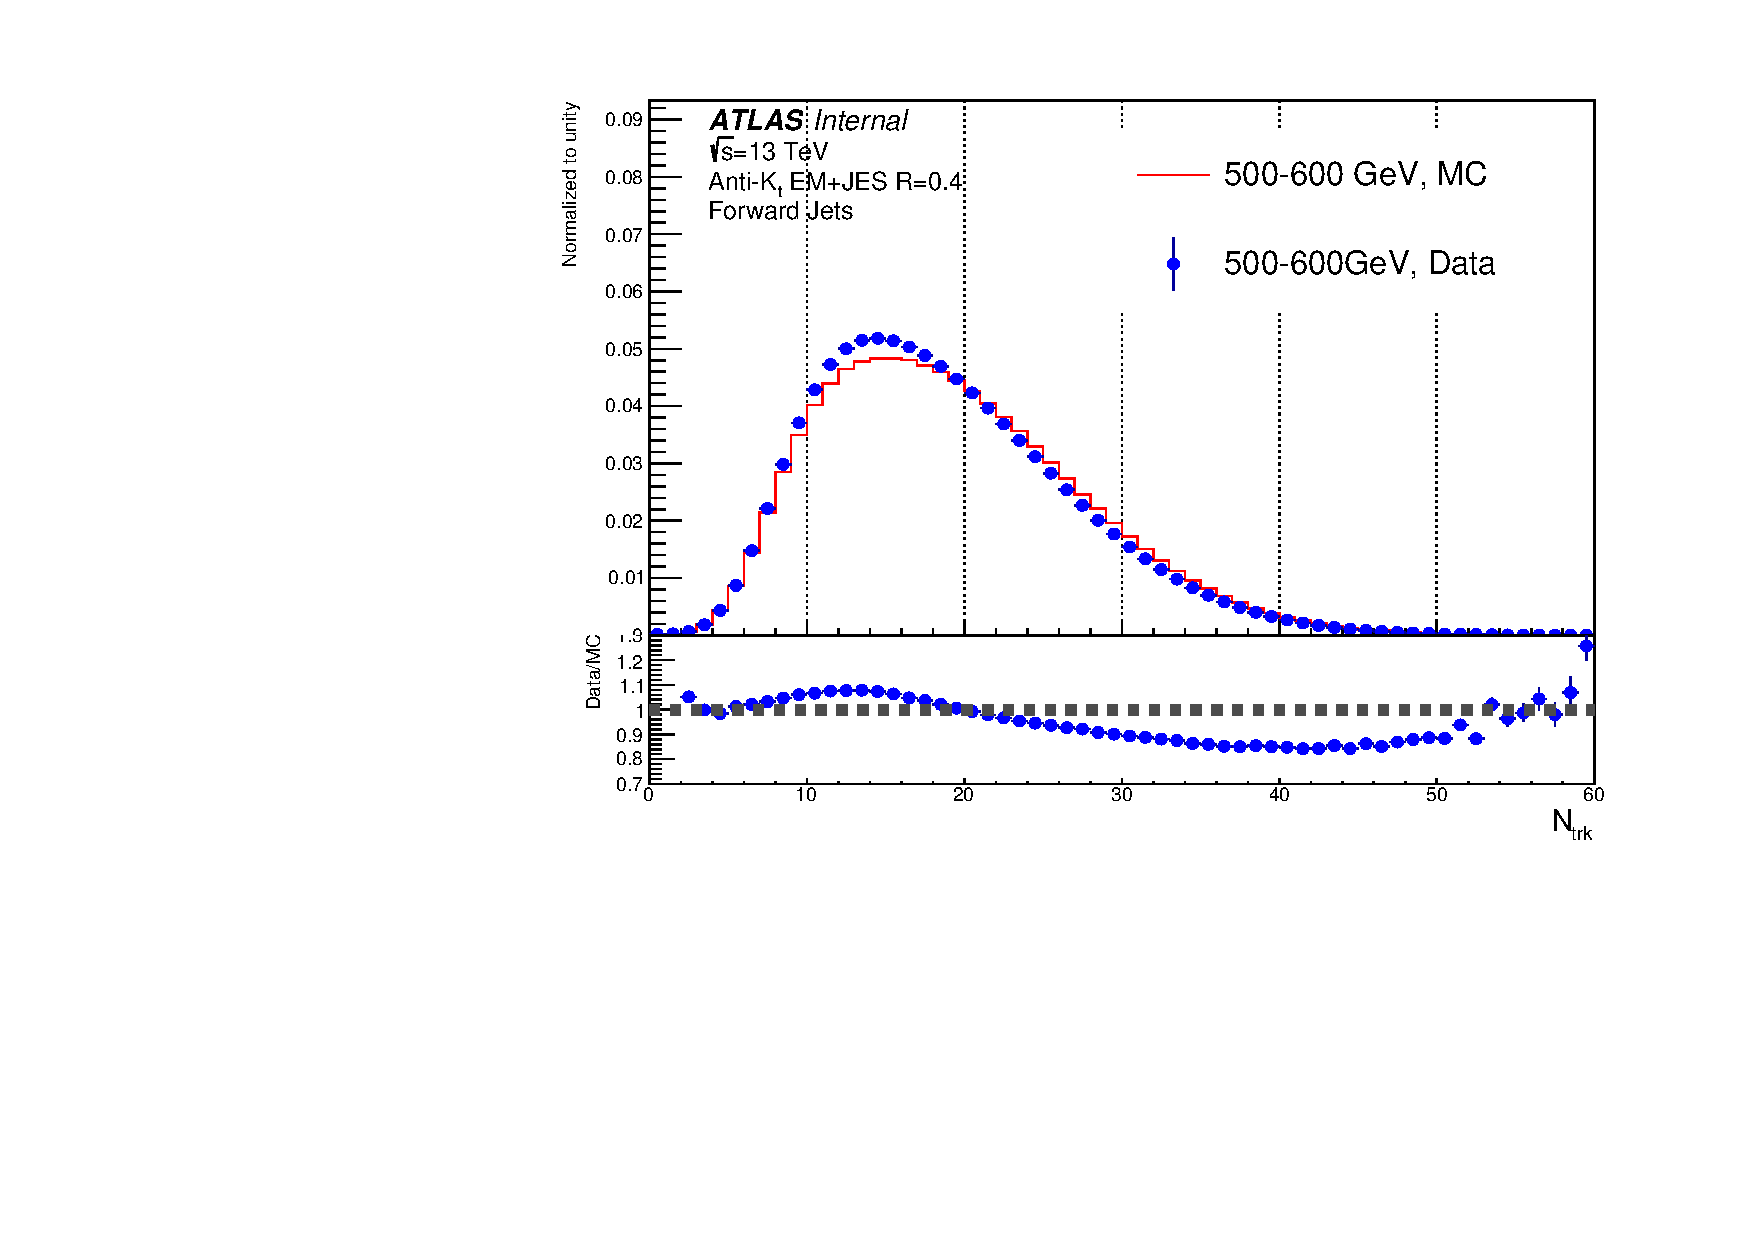
\includegraphics[width=0.45\textwidth]{fig/dijetanalysis/pythia-nominal/kinematics/ntrk_Forward_500_600_Pythia.pdf}} \quad
	\subfloat[Central region ]{\label{fig:QG-jetHLPtb}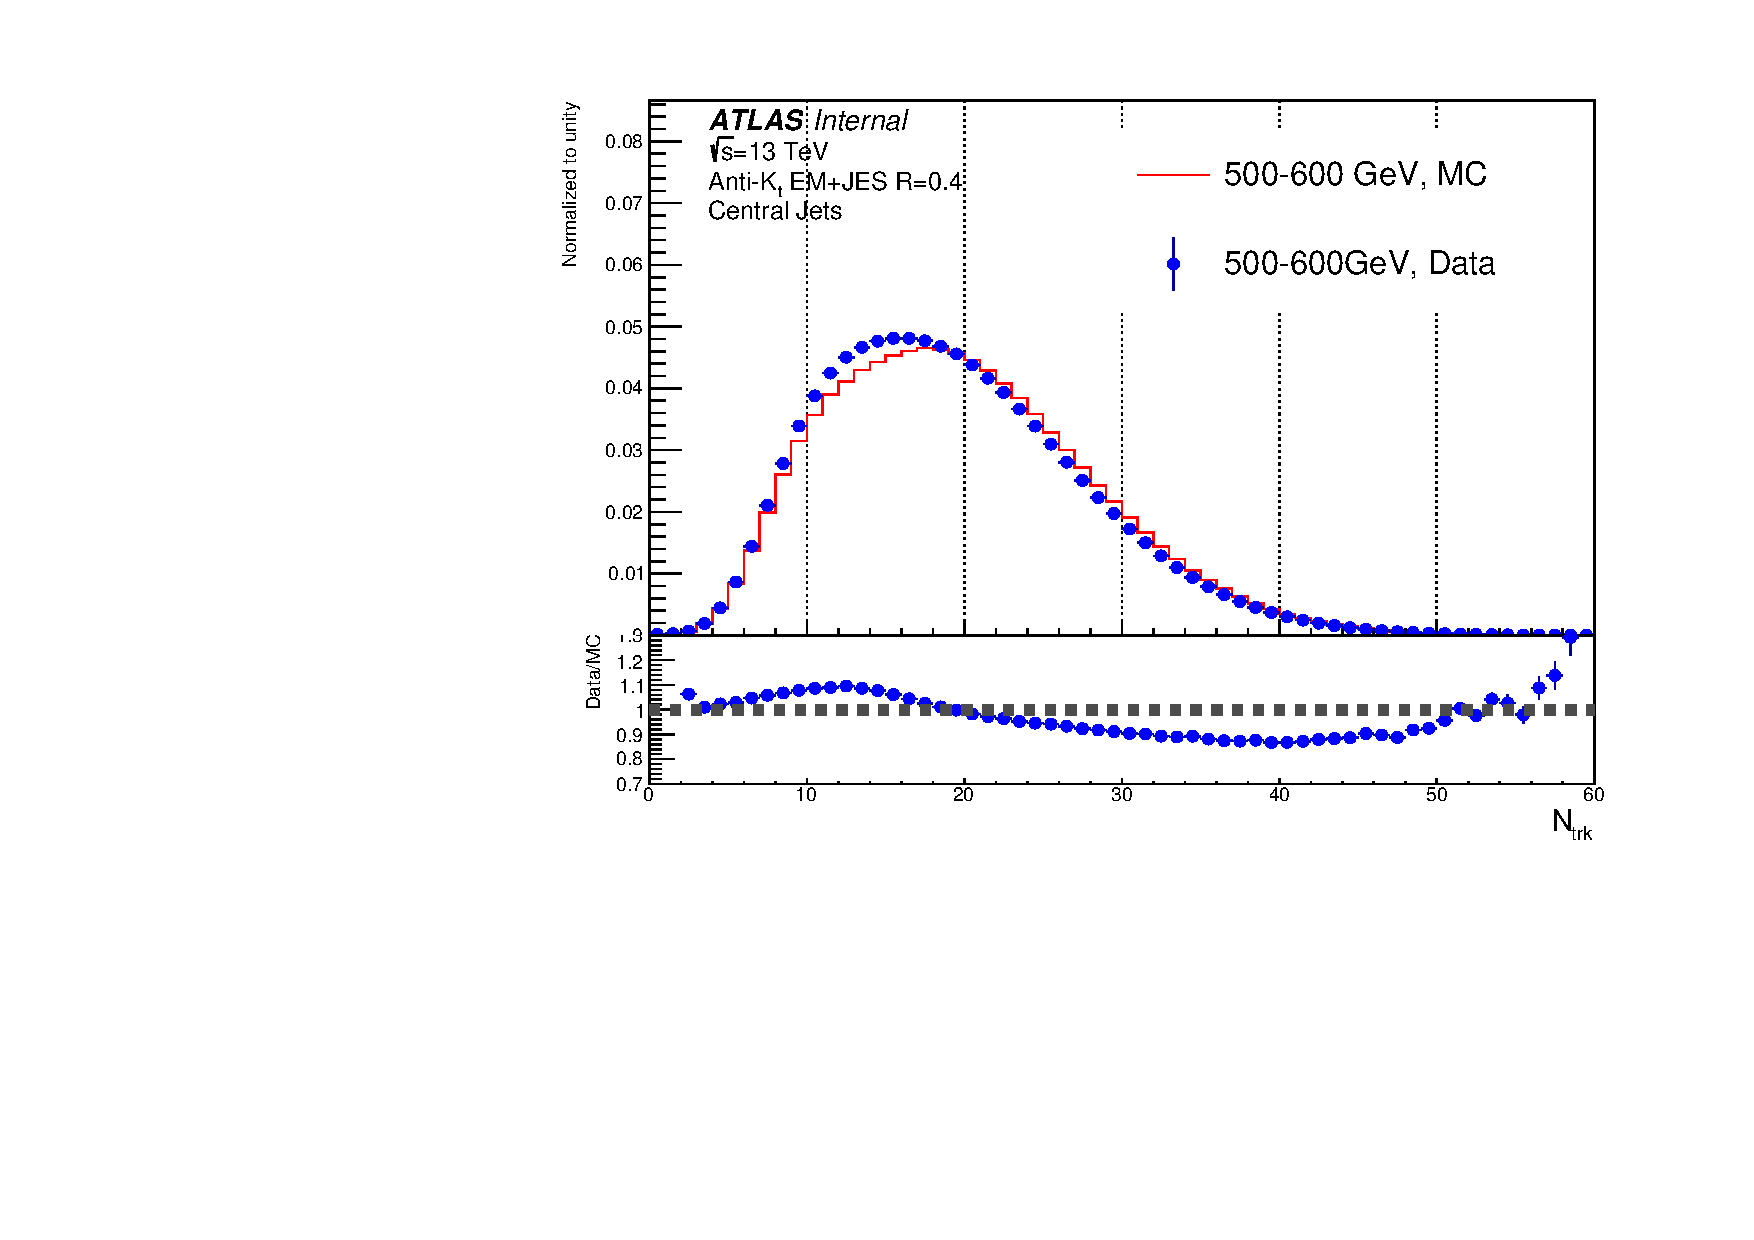
\includegraphics[width=0.45\textwidth]{fig/dijetanalysis/pythia-nominal/kinematics/ntrk_Central_500_600_Pythia.pdf}}\\
	\caption[]{
	  The \ntrk~distribution of the leading two jets with {\pythia8} in the MC and data.
		\label{fig:QG-ntrk-method1}
	}
\end{figure}

\begin{figure}[htb]
	\centering
	\subfloat[Forward region]{\label{fig:QG-jetHLPta}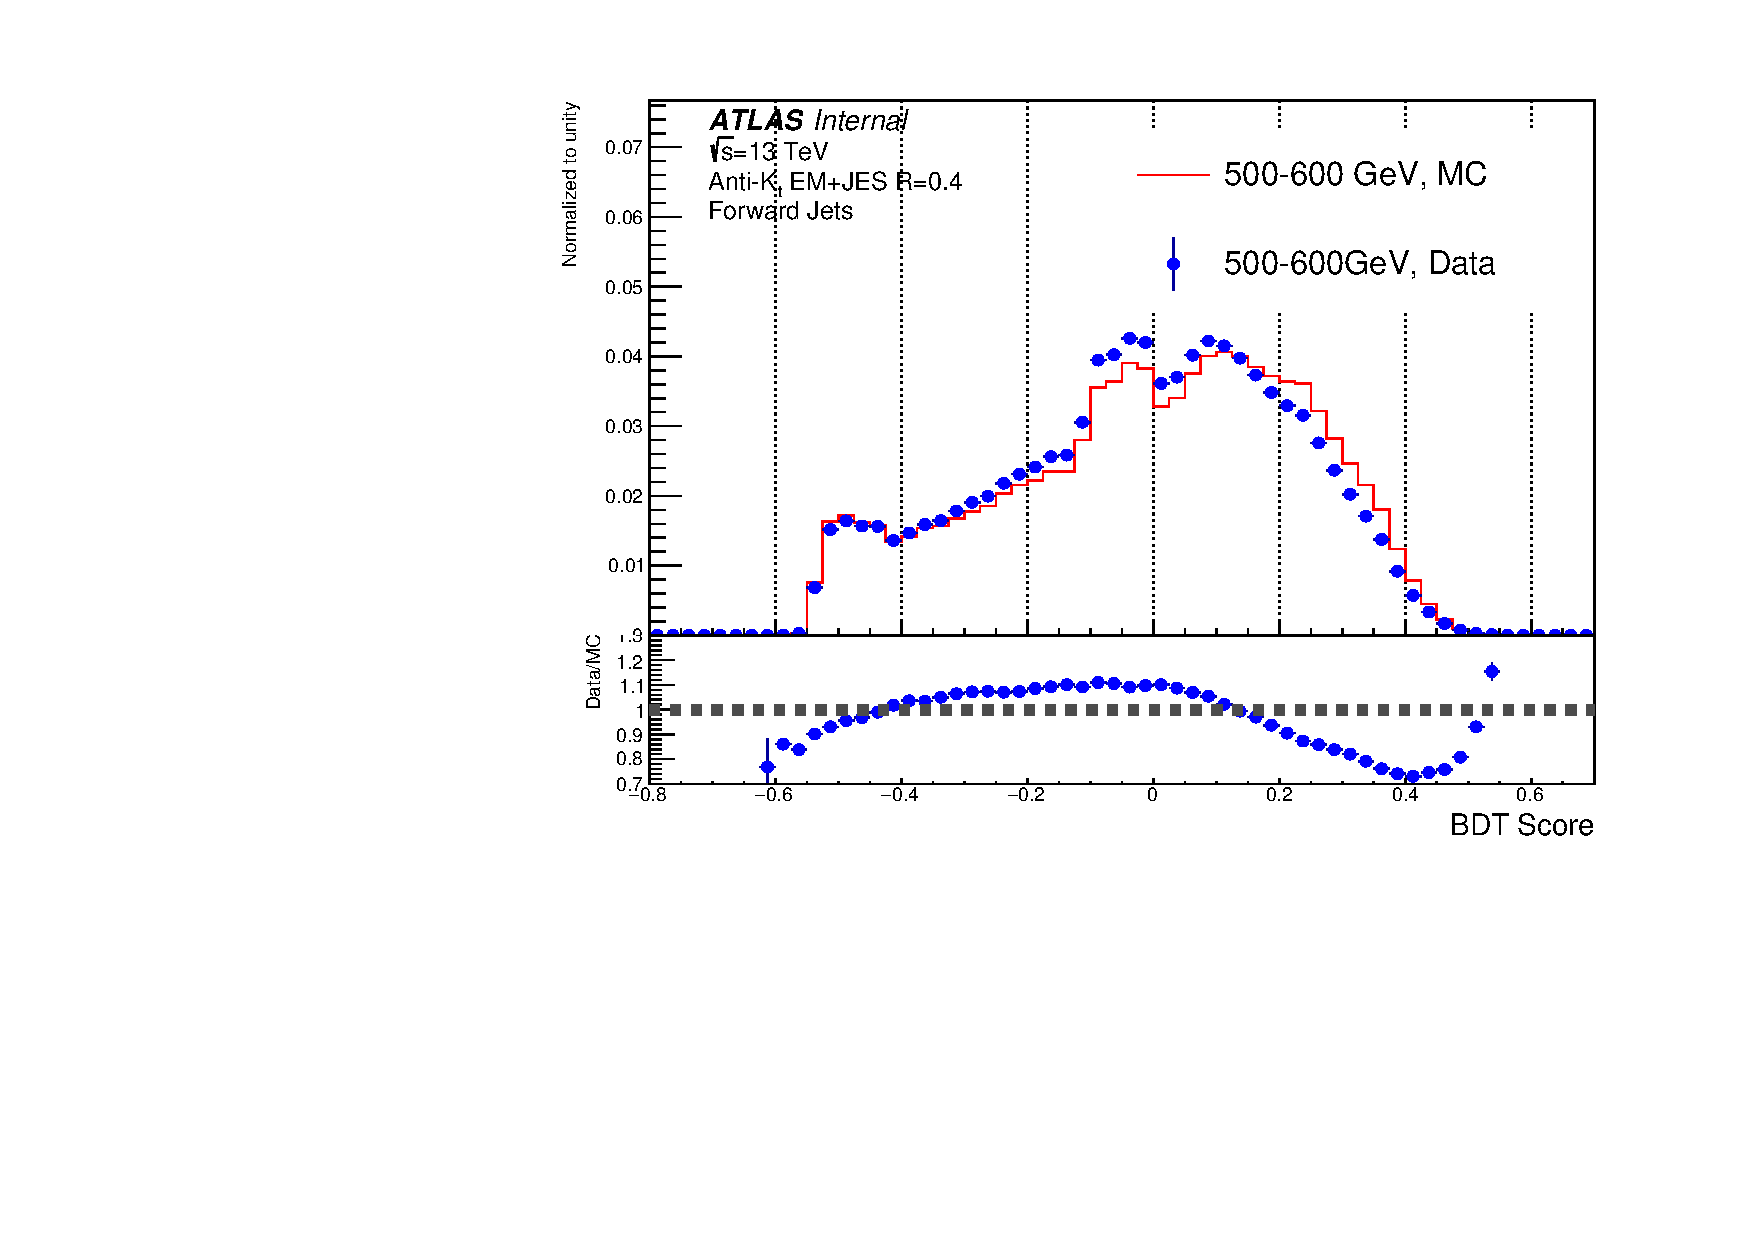
\includegraphics[width=0.45\textwidth]{fig/dijetanalysis/pythia-nominal/kinematics/bdt_Forward_500_600_Pythia.pdf}} \quad
	\subfloat[Central region ]{\label{fig:QG-jetHLPtb}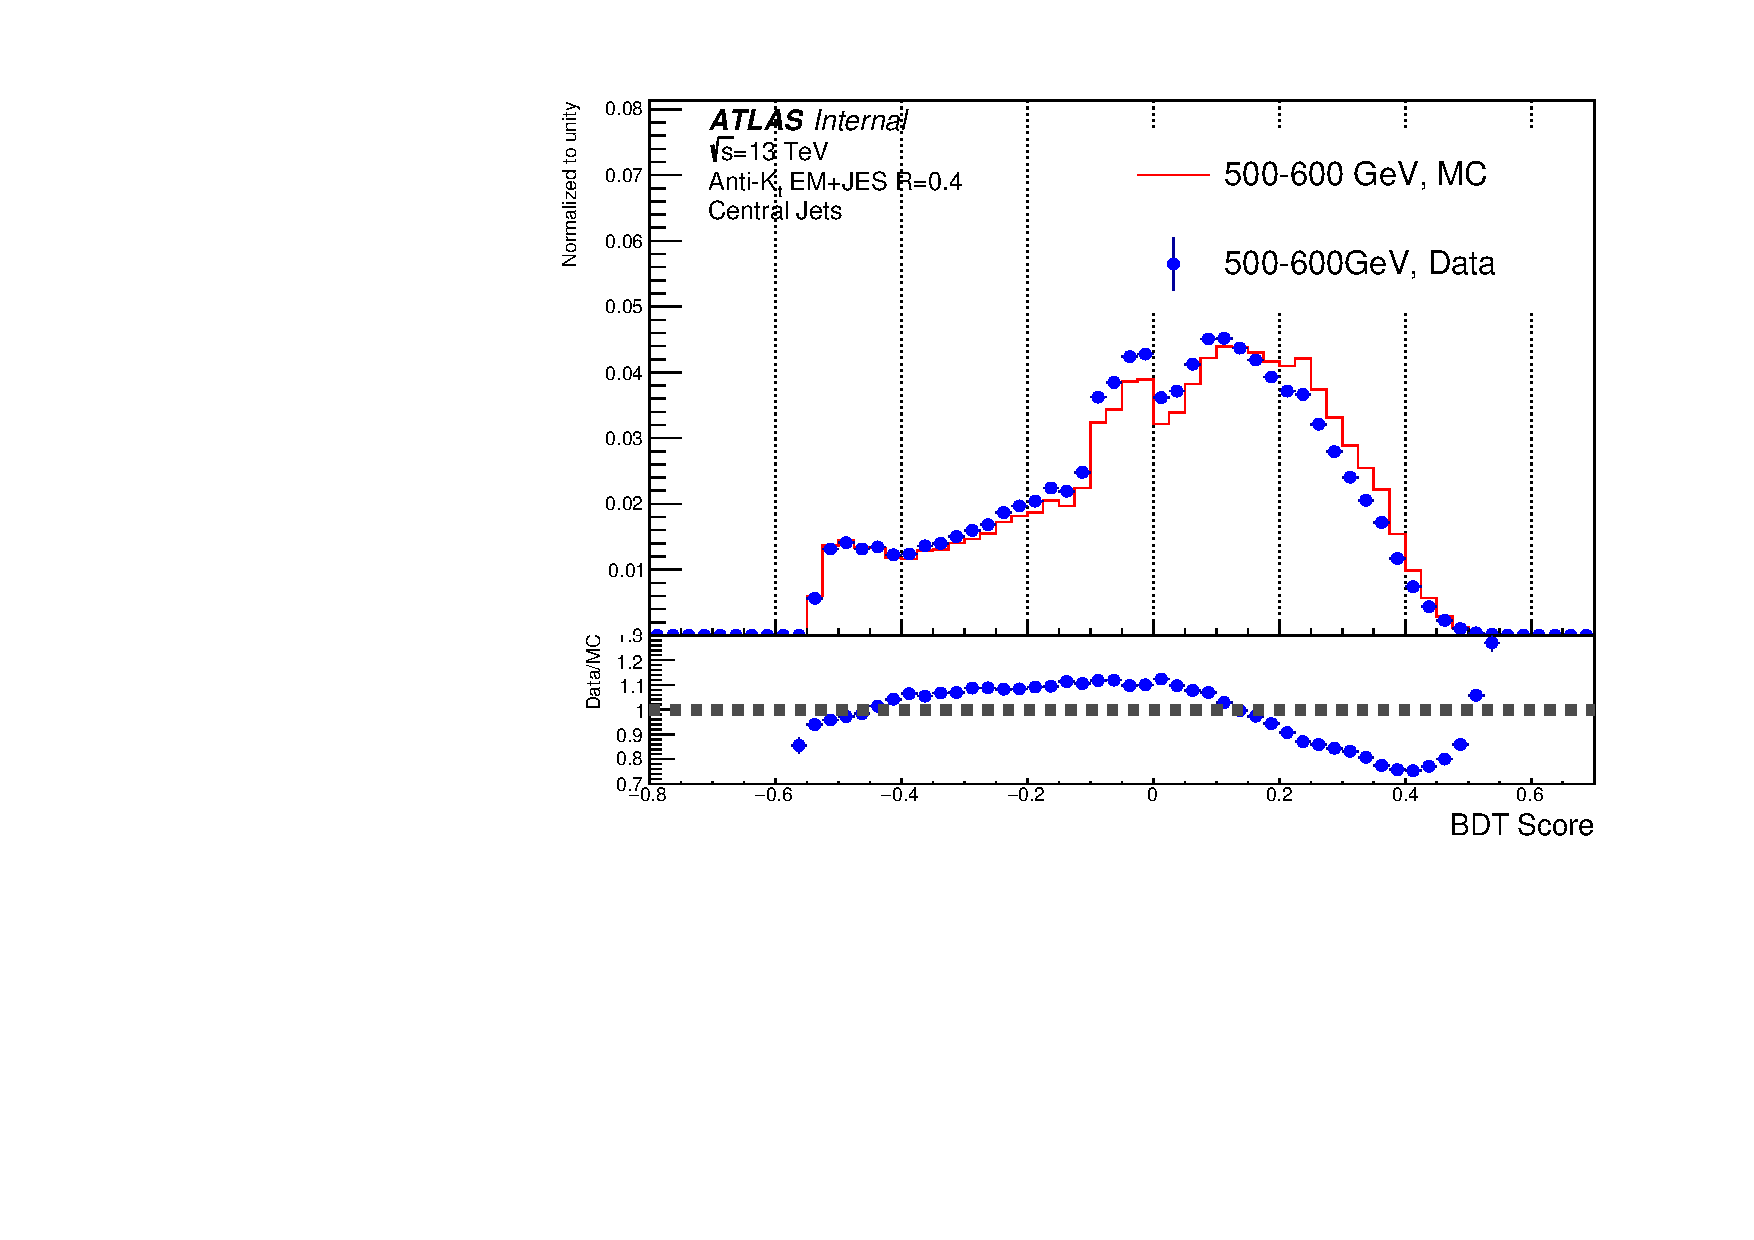
\includegraphics[width=0.45\textwidth]{fig/dijetanalysis/pythia-nominal/kinematics/bdt_Central_500_600_Pythia.pdf}}\\
	\caption[]{
	  The BDT score distribution of the leading two jets with {\pythia8} in the MC and data.
	    %Data for four plots are 139\ifb in total.	The normalization of the simulation is decided by cross-section.
		\label{fig:QG-jetHLPt}
	}
\end{figure}



%The matrix in 2-process extraction is given as 
%\begin{eqnarray}
%\label{eq:QG-matrix}
%\left(\begin{array}{c} 
%p_{\mrm{$\gamma$+jets}}(x)\\ 
%p_{\mrm{Multi-jet}}(x)\\ 
%\end{array}\right)
%&=&
%\underbrace{
%	\left(\begin{array}{cc}
%	f_{\mrm{$\gamma$+jets,Q}}&f_{\mrm{$\gamma$+jets,G}}\\
%	f_{\mrm{Multi-jet,Q}}&f_{\mrm{Multi-jet,G}}\\
%	\end{array}\right)
%}_{\scalebox{1}{$\equiv F$}}
%\left(\begin{array}{c} 
%p_\mrm{Q}(x)\\ 
%p_\mrm{G}(x)\\ 
%\end{array}\right)
%\\
%\label{eq:QG-invmatrix}
%\Leftrightarrow
%\left(\begin{array}{c} 
%p_\mrm{Q}(x)\\ 
%p_\mrm{G}(x)\\ 
%\end{array}\right)
%&=& F^{-1}
%\left(\begin{array}{c} 
%p_{\mrm{$\gamma$+jets}}(x)\\ 
%p_{\mrm{Multi-jet}}(x)\\ 
%\end{array}\right),
%\end{eqnarray}




%To estimate the systematic uncertainty coming from the parton shower modeling, %
%this calibration is performed for \pythia8 and \sherpa~separately. %
%%For \pythia8, both of the $Z$+jets and multi-jet MCs are \pythia8. %
%%For \sherpa, the $Z$+jets MC is \sherpa2.2.1 and the multi-jet MC is \sherpa2.1.1. %
%%This difference will be taken into account in the systematic uncertainties. %
%In \Sectrange{sec:QG-method}{sec:QG-SF}, the figures using \pythia8~(\sherpa) show results %
%with  NNPDF30~(NNPDF30) and NNPDF23LO~(CT10) PDF sets for 2-process extraction and for higher/lower \abseta jet extraction, respectively. %

%In \Sectrange{sec:QG-var}{sec:QG-SF}, the figures show the result with the \pythia8 parton shower modeling
%and the NNPDF30 PDF set for 2-process extraction or NNPDF23LO set for higher/lower \abseta jet. %
%A14 tuned NNPDF23LO set. %




%\begin{tabular}{l|l|c|c|cc}
% \hline
% \multicolumn{2}{l|}{\multirow{3}{*}{Selection}}& \multirow{3}{*}{$\gamma$+jets sample} & \multicolumn{3}{c}{Multi-jet sample}  \\ 
% \hhline{~~~---}
% \multicolumn{2}{l|}{} &                        & For 2-process & Higher |\etaX| & Lower |\etaX| \\ 
% \multicolumn{2}{l|}{} &                        & extraction    & jet sample  & jet sample \\ \hline 
% & Trigger   & Single photon trigger & \multicolumn{3}{c}{Or of single jet triggers} \\ 
% & MC-specialized cut & - & \multicolumn{3}{c}{$0.5<p_{\mrm{T,avg}}(\mrm{jets})/p_{\mrm{T,truth}}(j_1)<1.5$} \\ 
% & Number of jets        &  $\geq1$ & \multicolumn{3}{c}{$\geq2$} \\ \hhline{~~~---}
%  & $\pt$($\gamma$)             & $>125$     &-   & \multicolumn{2}{c}{-}   \\ 
% & $\pt(j_1)$             & $>50$     &$>50$  &\multicolumn{2}{c}{$>500$} \\ 
%  & $\pt(j_1)/\pt(j_2)$   &  -       & -    & \multicolumn{2}{c}{$<1.5$} \\ 
% & $|\eta(j_1)|$         &  $<2.1$  & $<2.1$ & \multicolumn{2}{c}{$<2.1$}   \\ 
% & $|\eta(j_2)|$         &  -       & -      & \multicolumn{2}{c}{$<2.1$}   \\ \hline
% & Target parton         &  Quark   & Gluon  & Quark  & Gluon       \\ \hhline{~-----}
% & Used jet in $j_1$ or $j_2$ & Only $j_1$ & Only $j_1$ & Higher $|\etaX|$ jet & Lower $|\etaX|$ jet \\
% \hline
%\end{tabular}

%In a low \pt range~($<500\GeV$), the quark fraction of  $\gamma$+jets is high~($\sim75\%$) %
%and the difference between the quark fractions in  $\gamma$+jets and multi-jet is large~($30$--$50\%$), %
%but the quark fraction of higher \abseta jet is low~($\lesssim 50\%$). % 
%Thus, the $\gamma$+jets and multi-jet are used as quark/gluon-enriched samples in the low \pt range. %
%In a high \pt range~($>500\GeVX$), higher \abseta jet has a large fraction of quarks~($>60\%$). %
%Thus, in the low \pt range, the higher/lower \abseta jet samples are used\footnote{
%The low statistics of $\gamma$+jets sample in the higher \pt range is another reason to use the higher/lower \abseta jet samples. %
%}. %
%The fractions are obtained from \pythia8 and \sherpa, separately. %


%\subsection{Method 1 for high \pt jet}
%\label{sec:method1_intro}

%\subsubsection{Background study}
%{\textcolor{red}{Wanyun: please add the background study here and tell people the background for dijet is negiligible}}
%In the whole \pt range, b-quark jets and jets labeled "other" exist, but it is suppressed to be lower than a few \%, which can be ignored. The jets labeled "other" are jets mainly originating from pileup.


%\FloatBarrier

% Data v.s. MC comparison in inclusive gamma+jets or Multi-jet(2sample ext.)

%\begin{figure}[htb]
%	\centering
%	\subfloat[$100<\pt<150\GeV$~(\sherpa) ]{\label{fig:QG-NtrkDataMCinclSherpaa}\includegraphics[width=0.45\textwidth]{Figures/dijetgammajetanalysis/MC_Closure/dist_comparison_plots/100-150_dist_total_comparison_ntrk_sherpa}} \quad
%	\subfloat[$500<\pt<600\GeV$~(\sherpa)]{\label{fig:QG-NtrkDataMCinclSherpab}\includegraphics[width=0.45\textwidth]{Figures/dijetgammajetanalysis/MC_Closure/dist_comparison_plots/500-600_dist_total_comparison_ntrk_sherpa}}\\
%	\subfloat[$100<\pt<150\GeV$~(\pythia8) ]{\label{fig:QG-WtrkDataMCincla}\includegraphics[width=0.45\textwidth]{Figures/dijetgammajetanalysis/MC_Closure/dist_comparison_plots/100-150_dist_total_comparison_ntrk_pythia}} \quad
%	\subfloat[$500<\pt<600\GeV$~(\pythia8)]{\label{fig:QG-WtrkDataMCinclb}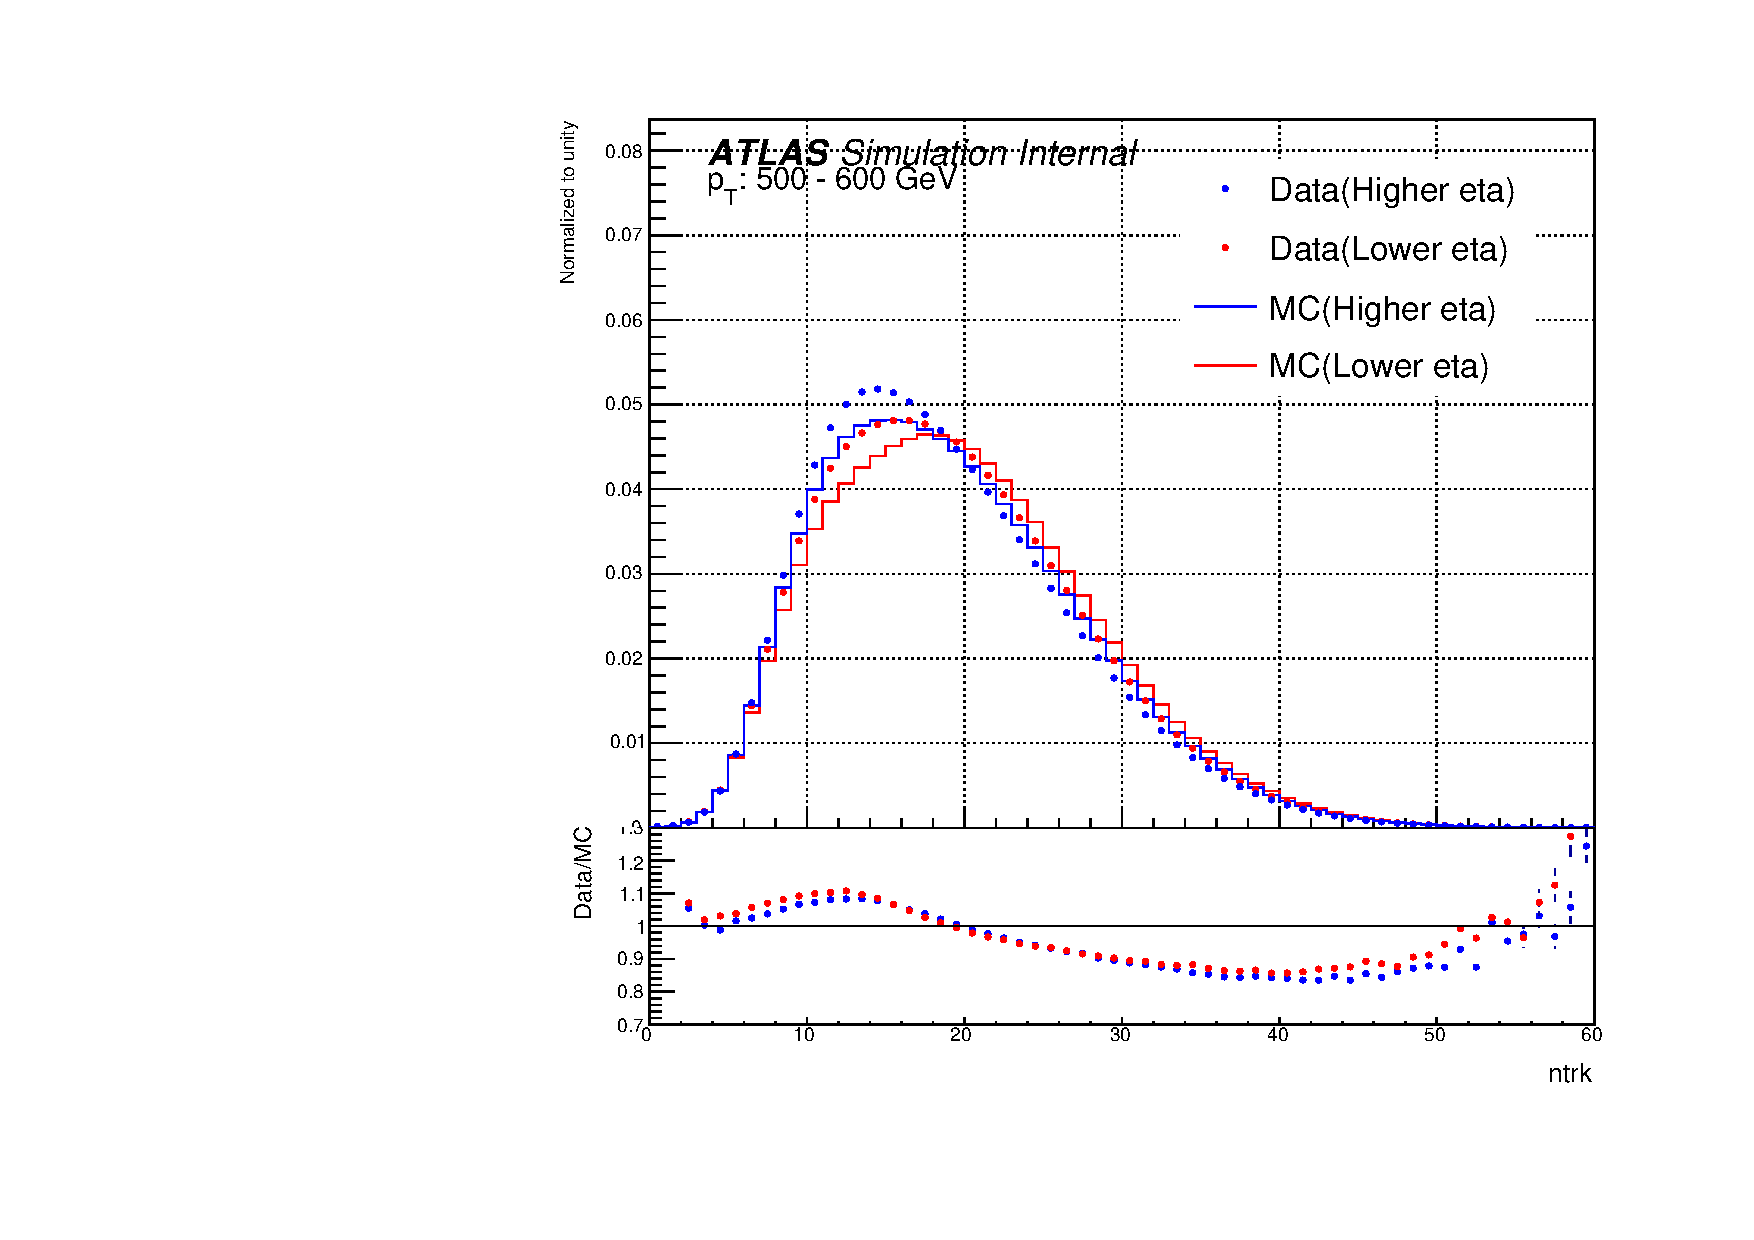
\includegraphics[width=0.45\textwidth]{Figures/dijetgammajetanalysis/MC_Closure/dist_comparison_plots/500-600_dist_total_comparison_ntrk_pythia}}
%	\caption[]{
%		The comparison between the data and MC with \sherpa  \subref{fig:QG-NtrkDataMCinclSherpaa} 	\subref{fig:QG-NtrkDataMCinclSherpab} and \pythia \subref{fig:QG-WtrkDataMCincla}  \subref{fig:QG-WtrkDataMCinclb} in \ntrk distributions of $\gamma$+jets and multi-jet events used in 2-sample extraction. %
%		Graphs and solid-line histograms show the \ntrk distributions in the data and MC, respectively.
%		Bottom panels show the ratio of the data to the MC in each of $\gamma$+jets and multi-jet events. %
%		\label{fig:QG-NtrkDataMCinclSherpa}
%	}
%\end{figure}
%
%\begin{figure}[htb]
%	\centering
%	\subfloat[$500<\pt<600\GeV$~(\sherpa) ]{\label{fig:QG-BDTDataMCinclSherpaa11}\includegraphics[width=0.45\textwidth]{Figures/dijetanalysis/higher-lower-sf/sherpa_MC_500_ntrk}} \quad
%	\subfloat[$800<\pt<1000\GeV$~(\sherpa)]{\label{fig:QG-BDTDataMCinclSherpab12}\includegraphics[width=0.45\textwidth]{Figures/dijetanalysis/higher-lower-sf/sherpa_MC_800_ntrk}}\\
%	\subfloat[$500<\pt<600\GeV$~(\pythia8) ]{\label{fig:QG-BDTDataMCinclPythiaa31}\includegraphics[width=0.45\textwidth]{Figures/dijetanalysis/higher-lower-sf/pythia_MC_500_ntrk}} \quad
%	\subfloat[$800<\pt<1000\GeV$~(\pythia8)]{\label{fig:QG-BDTDataMCinclPythiab41}\includegraphics[width=0.45\textwidth]{Figures/dijetanalysis/higher-lower-sf/pythia_MC_800_ntrk}}
%	\caption[]{
%		The comparison between the data and MC with \sherpa \subref{fig:QG-BDTDataMCinclSherpaa11} \subref{fig:QG-BDTDataMCinclSherpab21} and \pythia \subref{fig:QG-BDTDataMCinclPythiaa31} \subref{fig:QG-BDTDataMCinclPythiab41} in \nrtk distributions of higher or lower $\abseta$ multi-jet events used in 2-process extraction. %
%		Graphs and solid-line histograms show the \nrtk distributions in the data and MC, respectively.
%		Bottom panels show the ratio of the data to the MC in each of $\gamma$+jets and multi-jet events. %
%		\label{fig:QG-BDTDataMCinclPythia1}
%	}
%\end{figure}



%\begin{figure}[htb]
%	\centering
%	\subfloat[$50<\pt<600\GeV$~(\sherpa) ]{\label{fig:QG-WtrkDataMCinclaaa}\includegraphics[width=0.45\textwidth]{Figures/dijetanalysis/higher-lower-sf/sherpa_MC_500_ntrk}} \quad
%	\subfloat[$800<\pt<1000\GeV$~(\sherpa)]{\label{fig:QG-WtrkDataMCinclbbb}\includegraphics[width=0.45\textwidth]{Figures/dijetanalysis/higher-lower-sf/sherpa_MC_800_ntrk}}\\
%	\subfloat[$50<\pt<600\GeV$~(\pythia8) ]{\label{fig:QG-WtrkDataMCincla}\includegraphics[width=0.45\textwidth]{Figures/dijetanalysis/higher-lower-sf/pythia_MC_500_ntrk}} \quad
%	\subfloat[$800<\pt<1000\GeV$~(\pythia8)]{\label{fig:QG-WtrkDataMCinclb}\includegraphics[width=0.45\textwidth]{Figures/dijetanalysis/higher-lower-sf/pythia_MC_800_ntrk}}
%	\caption[]{
%		The comparison between the data and MC with \sherpa\subref{fig:QG-WtrkDataMCinclaaa} \subref{fig:QG-WtrkDataMCinclbbb} and \pythia \subref{fig:QG-WtrkDataMCincla} \subref{fig:QG-WtrkDataMCinclb} in \ntrk distributions of higher or lower $\abseta$ multi-jet events in 2-process extraction. %
%		Graphs and solid-line histograms show the \ntrk distributions in the data and MC, respectively.
%		Bottom panels show the ratio of the data to the MC in each of $\gamma$+jets and multi-jet events. %
%		\label{fig:QG-NtrkDataMCinclPythia}
%	}
%\end{figure}
%
%
%\begin{figure}[htb]
%	\centering
%	\subfloat[$100<\pt<150\GeV$~(\sherpa) ]{\label{fig:QG-WtrkDataMCinclSherpaa}\includegraphics[width=0.45\textwidth]{Figures/dijetgammajetanalysis/MC_Closure/dist_comparison_plots/100-150_dist_total_comparison_width_sherpa}} \quad
%	\subfloat[$500<\pt<600\GeV$~(\sherpa)]{\label{fig:QG-WtrkDataMCinclSherpab}\includegraphics[width=0.45\textwidth]{Figures/dijetgammajetanalysis/MC_Closure/dist_comparison_plots/500-600_dist_total_comparison_width_sherpa}}
%	\caption[]{
%		The comparison between the data and MC in \wtrk distributions of $\gamma$+jets and multi-jet events used in 2-sample extraction %
%		in \subref{fig:QG-WtrkDataMCinclSherpaa} the jet \pt range from 100 to 150\GeV and %
%		\subref{fig:QG-WtrkDataMCinclSherpab} from 500 to 600\GeV. %
%		Graphs and solid-line histograms show the \wtrk distributions in the data and MC, respectively.
%		Bottom panels show the ratio of the data to the MC in each of $\gamma$+jets and multi-jet events. %
%		\label{fig:QG-WtrkDataMCinclSherpa}
%	}
%\end{figure}
%
%\begin{figure}[htb]
%	\centering
%	\subfloat[$100<\pt<150\GeV$~(\pythia) ]{\label{fig:QG-WtrkDataMCinclSherpaa1}\includegraphics[width=0.45\textwidth]{Figures/dijetgammajetanalysis/MC_Closure/dist_comparison_plots/100-150_dist_total_comparison_width_pythia}} \quad
%	\subfloat[$500<\pt<600\GeV$~(\pythia)]{\label{fig:QG-WtrkDataMCinclSherpab1}\includegraphics[width=0.45\textwidth]{Figures/dijetgammajetanalysis/MC_Closure/dist_comparison_plots/500-600_dist_total_comparison_width_pythia}}
%	\caption[]{
%		The comparison between the data and MC in \wtrk distributions of $\gamma$+jets and multi-jet events used in 2-sample extraction %
%		in \subref{fig:QG-WtrkDataMCinclSherpaa} the jet \pt range from 100 to 150\GeV and %
%		\subref{fig:QG-WtrkDataMCinclSherpab} from 500 to 600\GeV. %
%		Graphs and solid-line histograms show the \wtrk distributions in the data and MC, respectively.
%		Bottom panels show the ratio of the data to the MC in each of $\gamma$+jets and multi-jet events. %
%		\label{fig:QG-WtrkDataMCinclSherpa1}
%	}
%\end{figure}
%
%\begin{figure}[htb]
%	\centering
%	\subfloat[$100<\pt<150\GeV$~(\sherpa) ]{\label{fig:QG-C1B02DataMCinclSherpaa}\includegraphics[width=0.45\textwidth]{Figures/dijetgammajetanalysis/MC_Closure/dist_comparison_plots/100-150_dist_total_comparison_c1_pythia}} \quad
%	\subfloat[$500<\pt<600\GeV$~(\sherpa)]{\label{fig:QG-C1B02DataMCinclSherpab}\includegraphics[width=0.45\textwidth]{Figures/dijetgammajetanalysis/MC_Closure/dist_comparison_plots/500-600_dist_total_comparison_c1_sherpa}}
%	\caption[]{
%		The comparison between the data and MC in \cbeta distributions of $\gamma$+jets and multi-jet events used in 2-sample extraction %
%		in \subref{fig:QG-C1B02DataMCinclSherpaa} the jet \pt range from 100 to 150\GeV and %
%		\subref{fig:QG-C1B02DataMCinclSherpab} from 500 to 600\GeV. %
%		Graphs and solid-line histograms show the \cbeta distributions in the data and MC, respectively.
%		Bottom panels show the ratio of the data to the MC in each of $\gamma$+jets and multi-jet events. %
%		\label{fig:QG-C1B02DataMCinclSherpa}
%	}
%\end{figure}
%
%\begin{figure}[htb]
%	\centering
%	\subfloat[$100<\pt<150\GeV$~(\pythia8) ]{\label{fig:QG-C1B02DataMCinclPythiaa}\includegraphics[width=0.45\textwidth]{Figures/dijetgammajetanalysis/MC_Closure/dist_comparison_plots/100-150_dist_total_comparison_c1_pythia}} \quad
%	\subfloat[$500<\pt<600\GeV$~(\pythia8)]{\label{fig:QG-C1B02DataMCinclPythiab}\includegraphics[width=0.45\textwidth]{Figures/dijetgammajetanalysis/MC_Closure/dist_comparison_plots/500-600_dist_total_comparison_c1_pythia}}
%	\caption[]{
%		The comparison between the data and MC in \cbeta distributions of $\gamma$ +jets and multi-jet events used in 2-sample extraction %
%		in \subref{fig:QG-C1B02DataMCinclPythiaa} the jet \pt range from 100 to 150\GeV and %
%		\subref{fig:QG-C1B02DataMCinclPythiab} from 500 to 600\GeV. %
%		Graphs and solid-line histograms show the \cbeta distributions in the data and MC, respectively.
%		Bottom panels show the ratio of the data to the MC in each of $\gamma$+jets and multi-jet events. %
%		\label{fig:QG-C1B02DataMCinclPythia}
%	}
%\end{figure}


%\begin{figure}[htb]
%	\centering
%	\subfloat[$100<\pt<150\GeV$~(\sherpa) ]{\label{fig:QG-BDTDataMCinclSherpaa}\includegraphics[width=0.45\textwidth]{Figures/dijetgammajetanalysis/MC_Closure/dist_comparison_plots/100-150_dist_total_comparison_bdt_sherpa}} \quad
%	\subfloat[$500<\pt<600\GeV$~(\sherpa)]{\label{fig:QG-BDTDataMCinclSherpab}\includegraphics[width=0.45\textwidth]{Figures/dijetgammajetanalysis/MC_Closure/dist_comparison_plots/500-600_dist_total_comparison_bdt_sherpa}}\\
%	\subfloat[$100<\pt<150\GeV$~(\pythia8) ]{\label{fig:QG-BDTDataMCinclPythiaa}\includegraphics[width=0.45\textwidth]{Figures/dijetgammajetanalysis/MC_Closure/dist_comparison_plots/100-150_dist_total_comparison_bdt_pythia}} \quad
%	\subfloat[$500<\pt<600\GeV$~(\pythia8)]{\label{fig:QG-BDTDataMCinclPythiab}\includegraphics[width=0.45\textwidth]{Figures/dijetgammajetanalysis/MC_Closure/dist_comparison_plots/500-600_dist_total_comparison_bdt_pythia}}
%	\caption[]{
%		The comparison between the data and MC with \sherpa \subref{fig:QG-BDTDataMCinclSherpaa} \subref{fig:QG-BDTDataMCinclSherpab} and \pythia \subref{fig:QG-BDTDataMCinclPythiaa} \subref{fig:QG-BDTDataMCinclPythiab}  in BDT distributions of $\gamma$+jets and multi-jet events used in 2-sample extraction.V. %
%		Graphs and solid-line histograms show the BDT distributions in the data and MC, respectively.
%		Bottom panels show the ratio of the data to the MC in each of $\gamma$+jets and multi-jet events. %
%		\label{fig:QG-BDTDataMCinclSherpa}
%	}
%\end{figure}
%\begin{figure}[htb]
%	\centering
%\subfloat[$500<\pt<600\GeV$~(\sherpa) ]{\label{fig:QG-BDTDataMCinclSherpaa1}\includegraphics[width=0.45\textwidth]{Figures/dijetanalysis/higher-lower-sf/sherpa_MC_500_bdt}} \quad
%\subfloat[$800<\pt<1000\GeV$~(\sherpa)]{\label{fig:QG-BDTDataMCinclSherpab2}\includegraphics[width=0.45\textwidth]{Figures/dijetanalysis/higher-lower-sf/sherpa_MC_800_bdt}}\\
%\subfloat[$500<\pt<600\GeV$~(\pythia8) ]{\label{fig:QG-BDTDataMCinclPythiaa3}\includegraphics[width=0.45\textwidth]{Figures/dijetanalysis/higher-lower-sf/pythia_MC_500_bdt}} \quad
%\subfloat[$800<\pt<1000\GeV$~(\pythia8)]{\label{fig:QG-BDTDataMCinclPythiab4}\includegraphics[width=0.45\textwidth]{Figures/dijetanalysis/higher-lower-sf/pythia_MC_800_bdt}}
%	\caption[]{
%		The comparison between the data and MC with \sherpa \subref{fig:QG-BDTDataMCinclSherpaa1} \subref{fig:QG-BDTDataMCinclSherpab2} and \pythia \subref{fig:QG-BDTDataMCinclPythiaa3} \subref{fig:QG-BDTDataMCinclPythiab4} in BDT distributions of higher or lower $\abseta$ multi-jet events used in 2-process extraction. %
%		Graphs and solid-line histograms show the BDT distributions in the data and MC, respectively.
%		Bottom panels show the ratio of the data to the MC in each of $\gamma$+jets and multi-jet events. %
%		\label{fig:QG-BDTDataMCinclPythia}
%	}
%\end{figure}

%\subsection{Method 2 for low \pt jet}
%\label{sec:method2_intro}
%\subsubsection{Prescale trigger}
%{\textcolor{red}{Wanyun and Rongqian: please add the study of prescale here for low pt dijet events}}
%The ATLAS trigger system consists of a hardware-based component, the Level-1 (L1), a software-based trigger system, the higher-level trigger (HLT) or Event Filter (EF). The HLT runs a simplified version of the ATLAS reconstruction software. On the HLT-level calibrated jets defined by the anti-kt algorithm with R = 0.4 are used. The calibration is close to the one of off-line jets. In this note the performance is evaluated with respect to PFlow jets.
%Each trigger item uses a L1 trigger and a HLT trigger. The L1 system first evaluates for each given trigger if it is passed. To keep the trigger rate at an acceptable level, the triggers with high trigger rate are only read-out for a fraction of all events ("prescales”). The prescale is a number applied on-line by the ATLAS trigger system. If an event passes the conditions set by the trigger system, the prescale for the L1 trigger and for the HLT trigger is decided. If the L1 or the HLT trigger is prescaled the HLT trigger decision is not evaluated in order to save computing time. The prescales for the L1 trigger and the HLT trigger are decided independently.
%The composition of the triggers used here is summarized in \Tab{tab:prescaletrigger}
%The jet \pT spectra for each of the triggers are shown in .{\textcolor{red}{Rongqian: please link jet triggers spectrum (before unprescaling) here}}\ref{fig:QG-b-ps}
%
%\begin{figure}[htb]
%	\centering
%	\subfloat[2017]{\label{fig:QG-2017ps}\includegraphics[width=0.45\textwidth]{Figures/Method2/Triggers/data17_single_trigger_Inclusive.pdf}}\quad
%	\subfloat[2018]{\label{fig:QG-2018ps}\includegraphics[width=0.45\textwidth]{Figures/Method2/Triggers/data18_single_trigger_Inclusive.pdf}}
%	\caption[]{
%	  The spectra for each jet trigger before unprescaling \subref{fig:QG-2017ps} is the 2017 dataset and \subref{fig:QG-b-ps} is the 2018 dataset.%
%		\label{fig:QG-b-ps}
%	}
%\end{figure}
%
%The jet \pT spectra can be corrected by the average prescale calculated by the ratio of luminosity collected by a given trigger and the total luminosity. The values in \href{https://aiatlas046.cern.ch/tagservices/RunBrowser/runBrowserReport/runBrowserReport.php?fnt=data18_13TeV&pn=*&cn=*}{COMA trigger report}are used. The corrected jet \pT spectra for each trigger are shown{\textcolor{red}{Rongqian: please link jet triggers spectrum (after unprescaling) here}}\ref{fig:QG-a-ps}
%
%\begin{figure}[htb]
%	\centering
%	\subfloat[2017]{\label{fig:QG-2017ps}\includegraphics[width=0.45\textwidth]{Figures/Method2/Triggers/data17single_trigger_InclusivePS.pdf}}\quad
%	\subfloat[2018]{\label{fig:QG-2018ps}\includegraphics[width=0.45\textwidth]{Figures/Method2/Triggers/data18single_trigger_InclusivePS.pdf}}
%	\caption[]{
%	  The spectra for each jet trigger after unprescaling \subref{fig:QG-2017ps} is the 2017 dataset and \subref{fig:QG-2018ps} is the 2018 dataset.%
%		\label{fig:QG-a-ps}
%	}
%\end{figure}
%
%\begin{table}[htb]
%	\centering
%	\caption{
%		The summary of the prescale HLT triggers used in this calibration. %
%	}
%	\begin{tabular}{c}
%		\whline
%		Trigger name \\
%		\hline
%		 HLT\_j35 \\
%		  HLT\_j45 \\
%		  HLT\_j60 \\
%		  HLT\_j110 \\
%		  HLT\_j175 \\
%		  HLT\_j260 \\
%		  HLT\_j360 \\
%		  \hline
%	 \end{tabular}
%	\label{tab:prescaletrigger}
%\end{table}
%
%
%
%{\textcolor{red}{Rongqian: please make the same plot in above section (method 1) for method 2 and put them here. Please put the plots in 100-150 and 400-500 GeV bins here and put others in appendix. }
%
%\begin{figure}[htb]
%	\centering
%	\subfloat[For $\gamma$+jets and multi-jet extraction~(\sherpa) ]{\label{fig:QG-Fmcc}\includegraphics[width=0.45\textwidth]{Figures/Method2/fraction/pt-fraction_pt.pdf}}\quad
%	\subfloat[For $\gamma$+jets and multi-jet extraction~(\pythia) ]{\label{fig:QG-Fmcd}\includegraphics[width=0.45\textwidth]{Figures/placeholder}}
%	\caption[]{
%	  (\textcolor{red}{Rongqian}) Fractions of quark jets and gluon jets in each of \subref{fig:QG-Fmcc} \subref{fig:QG-Fmcd} SHERPA and PYTHIA $\gamma$+jets and multi-jet for 2-process extraction %
%		$\gamma$+jets and multi-jets  %
%		These values are used as elements in $F$ matrix in \Eqn{eq:QG-matrix}(\ref{eq:QG-invmatrix}). %
%		\label{fig:QG-Fmc}
%	}
%\end{figure}
%
%
%\begin{figure}[htb]
%	\centering
%	\subfloat[$\gamma$+jets~(\sherpa)]{\label{fig:QG-jetMethod2Pta}\includegraphics[width=0.45\textwidth]{Figures/Method2/Pt-spectrum/GammaJet_Sherpa_pt_distribution.pdf}} \quad
%	\subfloat[multi-jet ~(\sherpa) ]{\label{fig:QG-jetHLPtb}\includegraphics[width=0.45\textwidth]{Figures/Method2/Pt-spectrum/LeadingJet_Dijet_Inclusive.png}}\\
%	\subfloat[$\gamma$+jets~(\pythia)]{\label{fig:QG-jetMethod2Ptaa}\includegraphics[width=0.45\textwidth]{Figures/placeholder}} \quad
%	\subfloat[multi-jet ~(\pythia) ]{\label{fig:QG-jetMethod2Ptbb}\includegraphics[width=0.45\textwidth]{Figures/placeholder}}
%%	\subfloat[$\gamma$+jets~(\sherpa)]{\label{fig:QG-jetMethod2Pta}\includegraphics[width=0.45\textwidth]{Figures/newplot/sherpa_higher_pt}} \quad
%%	\subfloat[multi-jet ~(\sherpa) ]{\label{fig:QG-jetMethod2Ptb}\includegraphics[width=0.45\textwidth]{Figures/newplot/sherpa_lower_pt}}\\
%%	\subfloat[$\gamma$+jets~(\pythia)]{\label{fig:QG-jetMethod2Ptaa}\includegraphics[width=0.45\textwidth]{Figures/dijetanalysis/pt-spectrum/powpyt_higher_pt}} \quad
%%	\subfloat[multi-jet ~(\pythia) ]{\label{fig:QG-jetMethod2Ptbb}\includegraphics[width=0.45\textwidth]{Figures/dijetanalysis/pt-spectrum/powpyt_lower_pt}}
%	\caption[]{
%	  (\textcolor{red}{Rongqian})The \pt distribution of the leading jets with \sherpa  \subref{fig:QG-jetMethod2Pta}  \subref{fig:QG-jetMethod2Ptb}  and \pythia 
%		 \subref{fig:QG-jetMethod2Ptaa}  \subref{fig:QG-jetMethod2Ptbb}  in  \subref{fig:QG-jetMethod2Pta} the $\gamma$+jets   %
%		and \subref{fig:QG-jetMethod2Ptb} the multi-jet extraction.
%	    %Data for four plots are 139\ifb in total.	The normalization of the simulation is decided by cross-section.
%		\label{fig:QG-jetMethod2Pt}
%	}
%\end{figure}
%
%\begin{figure}[htb]
%	\centering
%	\subfloat[$\gamma$+jets~(\sherpa)]{\label{fig:QG-jetHLPta}\includegraphics[width=0.45\textwidth]{Figures/Method2/kinematics/Gammajet-eta.png}} \quad
%	\subfloat[multi-jet~(\sherpa) ]{\label{fig:QG-jetHLPtb}\includegraphics[width=0.45\textwidth]{Figures/Method2/kinematics/Dijet_Sherpa_eta.png}}\\
%	\subfloat[$\gamma$+jets~(\pythia)]{\label{fig:QG-jetHLPtaa}\includegraphics[width=0.45\textwidth]{Figures/placeholder}} \quad
%	\subfloat[multi-jet~(\pythia) ]{\label{fig:QG-jetHLPtbb}\includegraphics[width=0.45\textwidth]{Figures/placeholder}}
%%	\subfloat[$\gamma$+jets~(\sherpa)]{\label{fig:QG-jetHLPta}\includegraphics[width=0.45\textwidth]{Figures/newplot/sherpa_higher_pt}} \quad
%%	\subfloat[Lower \abseta jet~(\sherpa) ]{\label{fig:QG-jetHLPtb}\includegraphics[width=0.45\textwidth]{Figures/newplot/sherpa_lower_pt}}\\
%%	\subfloat[Higher \abseta jet~(\pythia)]{\label{fig:QG-jetHLPtaa}\includegraphics[width=0.45\textwidth]{Figures/dijetanalysis/pt-spectrum/powpyt_higher_pt}} \quad
%%	\subfloat[Lower \abseta jet~(\pythia) ]{\label{fig:QG-jetHLPtbb}\includegraphics[width=0.45\textwidth]{Figures/dijetanalysis/pt-spectrum/powpyt_lower_pt}}
%	\caption[]{
%	  (\textcolor{red}{Rongqian})The \eta distribution of the jets with \sherpa  \subref{fig:QG-jetHLPta}  \subref{fig:QG-jetHLPtb}  and \pythia 
%		 \subref{fig:QG-jetHLPtaa}  \subref{fig:QG-jetHLPtbb}  in  \subref{fig:QG-jetHLPta} the $\gamma$+jets   %
%		and \subref{fig:QG-jetHLPtb} the multi-jet extraction.
%	    %Data for four plots are 139\ifb in total.	The normalization of the simulation is decided by cross-section.
%		\label{fig:QG-eta-method1}
%	}
%\end{figure}
%
%\begin{figure}[htb]
%	\centering
%	\subfloat[$\gamma$+jets~(\sherpa)]{\label{fig:QG-jetHLPta}\includegraphics[width=0.45\textwidth]{Figures/Method2/kinematics/Gammajet-ntrk.png}} \quad
%	\subfloat[multi-jet~(\sherpa) ]{\label{fig:QG-jetHLPtb}\includegraphics[width=0.45\textwidth]{Figures/Method2/kinematics/Dijet_Sherpa_ntrk.png}}\\
%	\subfloat[$\gamma$+jets~(\pythia)]{\label{fig:QG-jetHLPtaa}\includegraphics[width=0.45\textwidth]{Figures/placeholder}} \quad
%	\subfloat[multi-jet~(\pythia) ]{\label{fig:QG-jetHLPtbb}\includegraphics[width=0.45\textwidth]{Figures/placeholder}}
%%	\subfloat[Higher \abseta jet~(\sherpa)]{\label{fig:QG-jetHLPta}\includegraphics[width=0.45\textwidth]{Figures/newplot/sherpa_higher_pt}} \quad
%%	\subfloat[Lower \abseta jet~(\sherpa) ]{\label{fig:QG-jetHLPtb}\includegraphics[width=0.45\textwidth]{Figures/newplot/sherpa_lower_pt}}\\
%%	\subfloat[Higher \abseta jet~(\pythia)]{\label{fig:QG-jetHLPtaa}\includegraphics[width=0.45\textwidth]{Figures/dijetanalysis/pt-spectrum/powpyt_higher_pt}} \quad
%%	\subfloat[Lower \abseta jet~(\pythia) ]{\label{fig:QG-jetHLPtbb}\includegraphics[width=0.45\textwidth]{Figures/dijetanalysis/pt-spectrum/powpyt_lower_pt}}
%	\caption[]{
%	  (\textcolor{red}{Rongqian})The \ntrk distribution of the jets with \sherpa  \subref{fig:QG-jetHLPta}  \subref{fig:QG-jetHLPtb}  and \pythia 
%		 \subref{fig:QG-jetHLPtaa}  \subref{fig:QG-jetHLPtbb}  in  \subref{fig:QG-jetHLPta} the $\gamma$+jets   %
%		and \subref{fig:QG-jetHLPtb} the multi-jet extraction.
%	    %Data for four plots are 139\ifb in total.	The normalization of the simulation is decided by cross-section.
%		\label{fig:QG-ntrk-method1}
%	}
%\end{figure}
%
%\begin{figure}[htb]
%	\centering
%	\subfloat[$\gamma$+jets~(\sherpa)]{\label{fig:QG-jetHLPta}\includegraphics[width=0.45\textwidth]{Figures/Method2/kinematics/Gammajet-width.png}} \quad
%	\subfloat[multi-jet~(\sherpa) ]{\label{fig:QG-jetHLPtb}\includegraphics[width=0.45\textwidth]{Figures/Method2/kinematics/Dijet_Sherpa_width.png}}\\
%	\subfloat[$\gamma$+jets~(\pythia)]{\label{fig:QG-jetHLPtaa}\includegraphics[width=0.45\textwidth]{Figures/placeholder}} \quad
%	\subfloat[multi-jet~(\pythia) ]{\label{fig:QG-jetHLPtbb}\includegraphics[width=0.45\textwidth]{Figures/placeholder}}
%%	\subfloat[Higher \abseta jet~(\sherpa)]{\label{fig:QG-jetHLPta}\includegraphics[width=0.45\textwidth]{Figures/newplot/sherpa_higher_pt}} \quad
%%	\subfloat[Lower \abseta jet~(\sherpa) ]{\label{fig:QG-jetHLPtb}\includegraphics[width=0.45\textwidth]{Figures/newplot/sherpa_lower_pt}}\\
%%	\subfloat[Higher \abseta jet~(\pythia)]{\label{fig:QG-jetHLPtaa}\includegraphics[width=0.45\textwidth]{Figures/dijetanalysis/pt-spectrum/powpyt_higher_pt}} \quad
%%	\subfloat[Lower \abseta jet~(\pythia) ]{\label{fig:QG-jetHLPtbb}\includegraphics[width=0.45\textwidth]{Figures/dijetanalysis/pt-spectrum/powpyt_lower_pt}}
%	\caption[]{
%	  (\textcolor{red}{Rongqian})The \wtrk distribution of the leading jets with \sherpa  \subref{fig:QG-jetHLPta}  \subref{fig:QG-jetHLPtb}  and \pythia 
%		 \subref{fig:QG-jetHLPtaa}  \subref{fig:QG-jetHLPtbb}  in  \subref{fig:QG-jetHLPta} the $\gamma$+jets   %
%		and \subref{fig:QG-jetHLPtb} the multi-jet extraction.
%	    %Data for four plots are 139\ifb in total.	The normalization of the simulation is decided by cross-section.
%		\label{fig:QG-wtrk-methed1}
%	}
%\end{figure}
%
%\begin{figure}[htb]
%	\centering
%	\subfloat[$\gamma$+jets~(\sherpa)]{\label{fig:QG-jetHLPta}\includegraphics[width=0.45\textwidth]{Figures/Method2/kinematics/Gammajet-c1.png}} \quad
%	\subfloat[multi-jet~(\sherpa) ]{\label{fig:QG-jetHLPtb}\includegraphics[width=0.45\textwidth]{Figures/Method2/kinematics/Dijet_Sherpa_c1.png}}\\
%	\subfloat[$\gamma$+jets~(\pythia)]{\label{fig:QG-jetHLPtaa}\includegraphics[width=0.45\textwidth]{Figures/placeholder}} \quad
%	\subfloat[multi-jet jet~(\pythia) ]{\label{fig:QG-jetHLPtbb}\includegraphics[width=0.45\textwidth]{Figures/placeholder}}
%%	\subfloat[Higher \abseta jet~(\sherpa)]{\label{fig:QG-jetHLPta}\includegraphics[width=0.45\textwidth]{Figures/newplot/sherpa_higher_pt}} \quad
%%	\subfloat[Lower \abseta jet~(\sherpa) ]{\label{fig:QG-jetHLPtb}\includegraphics[width=0.45\textwidth]{Figures/newplot/sherpa_lower_pt}}\\
%%	\subfloat[Higher \abseta jet~(\pythia)]{\label{fig:QG-jetHLPtaa}\includegraphics[width=0.45\textwidth]{Figures/dijetanalysis/pt-spectrum/powpyt_higher_pt}} \quad
%%	\subfloat[Lower \abseta jet~(\pythia) ]{\label{fig:QG-jetHLPtbb}\includegraphics[width=0.45\textwidth]{Figures/dijetanalysis/pt-spectrum/powpyt_lower_pt}}
%	\caption[]{
%	  (\textcolor{red}{Rongqian})The C1 distribution of the jets with \sherpa  \subref{fig:QG-jetHLPta}  \subref{fig:QG-jetHLPtb}  and \pythia 
%		 \subref{fig:QG-jetHLPtaa}  \subref{fig:QG-jetHLPtbb}  in  \subref{fig:QG-jetHLPta} the $\gamma$+jets   %
%		and \subref{fig:QG-jetHLPtb} the multi-jet extraction.
%	    %Data for four plots are 139\ifb in total.	The normalization of the simulation is decided by cross-section.
%		\label{fig:QG-wtrk-methed1}
%	}
%\end{figure}
%
%\begin{figure}[htb]
%	\centering
%	\subfloat[$100<\pt<150\GeV$~(\sherpa) ]{\label{fig:QG-NtrkDataMCinclSherpaa}\includegraphics[width=0.45\textwidth]{Figures/Method2/SF-MC/100-150_dist_total_comparison_ntrk_sherpa.pdf}} \quad
%	\subfloat[400<\pt<500\GeV$~(\sherpa)]{\label{fig:QG-NtrkDataMCinclSherpab}\includegraphics[width=0.45\textwidth]{Figures/Method2/SF-MC/400-500_dist_total_comparison_ntrk_sherpa.pdf}}\\
%	\subfloat[$100<\pt<150\GeV$~(\pythia8) ]{\label{fig:QG-WtrkDataMCincla}\includegraphics[width=0.45\textwidth]{Figures/Method2/SF-MC/}} \quad
%	\subfloat[$400<\pt<500\GeV$~(\pythia8)]{\label{fig:QG-WtrkDataMCinclb}\includegraphics[width=0.45\textwidth]{Figures/Method2/SF-MC/}}
%	\caption[]{
%		The comparison between the data and MC with \sherpa  \subref{fig:QG-NtrkDataMCinclSherpaa} 	\subref{fig:QG-NtrkDataMCinclSherpab} and \pythia \subref{fig:QG-WtrkDataMCincla}  \subref{fig:QG-WtrkDataMCinclb} in \ntrk distributions of $\gamma$+jets and multi-jet events used in 2-sample extraction. %
%		Graphs and solid-line histograms show the \ntrk distributions in the data and MC, respectively.
%		Bottom panels show the ratio of the data to the MC in each of $\gamma$+jets and multi-jet events. %
%		\label{fig:QG-NtrkDataMCinclSherpa}
%	}
%\end{figure}
%
%\begin{figure}[htb]
%	\centering
%	\subfloat[$100<\pt<150\GeV$~(\sherpa) ]{\label{fig:QG-NtrkDataMCinclSherpaa}\includegraphics[width=0.45\textwidth]{Figures/Method2/SF-MC/100-150_dist_total_comparison_bdt_sherpa.pdf}} \quad
%	\subfloat[400<\pt<500\GeV$~(\sherpa)]{\label{fig:QG-NtrkDataMCinclSherpab}\includegraphics[width=0.45\textwidth]{Figures/Method2/SF-MC/400-500_dist_total_comparison_bdt_sherpa.pdf}}\\
%	\subfloat[$100<\pt<150\GeV$~(\pythia8) ]{\label{fig:QG-WtrkDataMCincla}\includegraphics[width=0.45\textwidth]{Figures/Method2/SF-MC/}} \quad
%	\subfloat[$400<\pt<500\GeV$~(\pythia8)]{\label{fig:QG-WtrkDataMCinclb}\includegraphics[width=0.45\textwidth]{Figures/Method2/SF-MC/}}
%	\caption[]{
%		The comparison between the data and MC with \sherpa  \subref{fig:QG-NtrkDataMCinclSherpaa} 	\subref{fig:QG-NtrkDataMCinclSherpab} and \pythia \subref{fig:QG-WtrkDataMCincla}  \subref{fig:QG-WtrkDataMCinclb} in BDT distributions of $\gamma$+jets and multi-jet events used in 2-sample extraction. %
%		Graphs and solid-line histograms show the BDT distributions in the data and MC, respectively.
%		Bottom panels show the ratio of the data to the MC in each of $\gamma$+jets and multi-jet events. %
%		\label{fig:QG-NtrkDataMCinclSherpa}
%	}
%\end{figure}
%
%\begin{figure}[htb]
%	\centering
%	\subfloat[$100<\pt<150\GeV$~(\sherpa) ]{\label{fig:QG-BDT1}\includegraphics[width=0.45\textwidth]{Figures/Method2/roc/plots/roc-var/ROC_100-150_dijet.pdf}} \quad
%	\subfloat[400<\pt<500\GeV$~(\sherpa)]{\label{fig:QG-BDT2}\includegraphics[width=0.45\textwidth]{Figures/Method2/roc/plots/roc-var/ROC_400-500_dijet.pdf}}\\
%	\subfloat[$100<\pt<150\GeV$~(\pythia8) ]{\label{fig:QG-WtrkDataMCincla}\includegraphics[width=0.45\textwidth]{Figures/Method2/SF-MC/}} \quad
%	\subfloat[$400<\pt<500\GeV$~(\pythia8)]{\label{fig:QG-WtrkDataMCinclb}\includegraphics[width=0.45\textwidth]{Figures/Method2/SF-MC/}}
%	\caption[]{
%		ROC curve for different jet taggers%
%		\label{fig:QG-NtrkDataMCinclSherpa}
%	}
%\end{figure}
%
%
%\subsubsection{Background study}
%{\textcolor{red}{Wanyun and Rongqian: please add the background study here (ABCD) and tell people the background for dijet is negiligible}}
%
%
%
%\subsection{Validation} (\textcolor{red}{let's skip this section for now})
%\label{subsec:Validation }
%
%In addition to the primary samples defined above, several samples with very high quark or gluon-jet fractions are defined to validate the extracted templates in different topologies. The high purity is achieved by the use of event-level kinematic cuts. One is trijet sample used for validation of the extracted gluon template, Events are required to have a leading jet which passes the lowest unprescaled single jet trigger and a pT of at least 500 GeV. There must be at least two additional jets with \pT $>$ 20 GeV. All three jets must have $\abseta$ $<$ 2.1. The third jet is very likely to be gluon initiated in certain regions of phase space. The other one is $\gamma$+2jets sample, which has high quark-jet purity,The basic event selection is the same as for the $\gamma$+jet sample, with the exceptions that there should be at least one sub-leading jet with \pT > 20 GeV and $\abseta$ $<$ 2.1. 
\FloatBarrier


\subsection{MC non-closure}
\label{sec:QG-closure}
 
  The matrix method is valid under the assumption that the shapes of $p_{\mrm{Q}}(x)$ and $p_{\mrm{G}}(x)$ emain consistent, regardless of whether the jets are situated in the central or forward regions. Jet fragmentation at a $pp$ collider is expected to be predominantly influenced by the jet \pt~and is generally considered independent of $\eta$, considering the underlying parton type. Consequently, an approach aimed at extracting distributions associated with the radiation patterns of quark-jets and gluon-jets should be valid at the particle level. At the detector level, however, the measured radiation pattern within jets no longer retains its $\eta$-independence. This is due to variations arising from differences in detector materials and technologies, leading to distinctions between the central and forward regions in terms of response. As a consequence of these effects, the matrix method experiences deviations from closure,, indicating a disparity between the expected and actual outcomes.
  


The distributions of {\ntrk} have been seen to have systematic difference for the truth-labelled quark/gluon jets in the quark-enriched and gluon-enriched regions in each \pt~bin. To rectify this discrepancy and ensure alignment in the distribution of jet tagging variables between the central and forward regions, a re-weighting procedure is implemented. This procedure involves applying adjustments to account for the observed differences.  For each event, the central jet is weighted by a re-weighting factor :
\begin{equation}
%w_{\mrm{Q/G}}({x;p_{\text{T,j}}}) = \frac{ p_{\mrm{Q/G,~higher \abseta}}({x;p_{\text{T,j}}}) }{ p_{\mrm{Q/G,~lower \abseta}}({x;p_{\text{T,j}}})}
w_{\mathrm{Q} / \mathrm{G}}\left(x ; p_{\mathrm{T}, \mathrm{j}}\right)=\frac{p_{\mathrm{Q} / \mathrm{G}, \text { forward }}\left(x ; p_{\mathrm{T}, \mathrm{j}}\right)}{p_{\mathrm{Q} / \mathrm{G}, \text { central }}\left(x ; p_{\mathrm{T}, \mathrm{j}}\right)}
\label{eq:QG-reweight}
\end{equation}
where $q/g$ tagging variable $x$ is calculated in each jet \pt~bin for quark and gluon jets, respectively. By default the re-weighting factor derived from truth-labelled quark-jets is implemented for both types of jets, whereas the re-weighting factor derived from truth-labelled gluon-jets is used as an alternative to evaluate the systematic uncertainty from the re-weighting procedure, known as MC non-closure systematic uncertainty for the calibration.



The distributions of \ntrk~in extracted pure quark- and gluon-jets and truth-labelled MC before re-weighting as shown in Figure~\ref{fig:QG-pythia-NtrkMCExtractedNoReweight-Ntrk}. After the re-weighting the distributions of \ntrk~are shown in Figure~\ref{fig:QG-pythia-NtrkMCExtractedQuarkFactor-Ntrk}. The non-closure is at few percent level and is is taken as MC non-closure systematic uncertainty. 

\begin{figure}[htb]
	\centering
	\subfloat[ ]{\label{fig:QG-pythia-QuarkNtrkMCExtractedNoReweight-500-600-Ntrk}\includegraphics[width=0.45\textwidth]{fig/ADE/MCClosure/none_event_weight/jet_nTracks/MCClosure_500_quark_jet_nTracks.pdf}} \quad
	\subfloat[ ]{\label{fig:QG-pythia-GluonNtrkMCExtractedNoReweight-500-600-Ntrk}\includegraphics[width=0.45\textwidth]{fig/ADE/MCClosure/none_event_weight/jet_nTracks/MCClosure_500_gluon_jet_nTracks.pdf}} \\
	\subfloat[ ]{\label{fig:QG-pythia-QuarkNtrkMCExtractedNoReweight-800-1000-Ntrk}\includegraphics[width=0.45\textwidth]{fig/ADE/MCClosure/none_event_weight/jet_nTracks/MCClosure_800_quark_jet_nTracks.pdf}} \quad
	\subfloat[ ]{\label{fig:QG-pythia-GluonNtrkMCExtractedNoReweight-800-1000-Ntrk}\includegraphics[width=0.45\textwidth]{fig/ADE/MCClosure/none_event_weight/jet_nTracks/MCClosure_800_gluon_jet_nTracks.pdf}} \\
	\caption[]{
		Before re-weighting: the {\ntrk} distributions of quark-jet \subref{fig:QG-pythia-QuarkNtrkMCExtractedNoReweight-500-600-Ntrk}  \subref{fig:QG-pythia-QuarkNtrkMCExtractedNoReweight-800-1000-Ntrk} 
		and  gluon-jet in \subref{fig:QG-pythia-GluonNtrkMCExtractedNoReweight-500-600-Ntrk}  \subref{fig:QG-pythia-GluonNtrkMCExtractedNoReweight-800-1000-Ntrk} 
		 from {\pythia8} sample. %
		Dashed and solid-line show the {\ntrk} distributions in the truth MC and extracted MC, respectively.
		Bottom panels show the ratio of the extracted MC to the truth MC. %
		\label{fig:QG-pythia-NtrkMCExtractedNoReweight-Ntrk}
	}
\end{figure}



\begin{figure}[htb]
	\centering
	\subfloat[ ]{\label{fig:QG-pythia-QuarkNtrkMCExtractedQuarkFactor-Ntrk-500-600-Ntrk}\includegraphics[width=0.45\textwidth]{fig/ADE/MCClosure/jet_nTracks_quark_reweighting_weights/jet_nTracks/MCClosure_500_quark_jet_nTracks.pdf}} \quad
	\subfloat[ ]{\label{fig:QG-pythia-GluonNtrkMCExtractedQuarkFactor-Ntrk-500-600-Ntrk}\includegraphics[width=0.45\textwidth]{fig/ADE/MCClosure/jet_nTracks_quark_reweighting_weights/jet_nTracks/MCClosure_500_gluon_jet_nTracks.pdf}} \\
	\subfloat[ ]{\label{fig:QG-pythia-QuarkNtrkMCExtractedEQuarkFactor-Ntrk-800-1000-Ntrk}\includegraphics[width=0.45\textwidth]{fig/ADE/MCClosure/jet_nTracks_quark_reweighting_weights/jet_nTracks/MCClosure_800_quark_jet_nTracks.pdf}} \quad
	\subfloat[ ]{\label{fig:QG-pythia-GluonNtrkMCExtractedQuDarkFactor-Ntrk-800-1000-Ntrk}\includegraphics[width=0.45\textwidth]{fig/ADE/MCClosure/jet_nTracks_quark_reweighting_weights/jet_nTracks/MCClosure_800_gluon_jet_nTracks.pdf}} \\
	\caption[]{
		After re-weighting with quark factor: the {\ntrk} distributions of quark-jet \subref{fig:QG-pythia-QuarkNtrkMCExtractedQuarkFactor-Ntrk-500-600-Ntrk} \subref{fig:QG-pythia-QuarkNtrkMCExtractedEQuarkFactor-Ntrk-800-1000-Ntrk} 
		and gluon-jet in \subref{fig:QG-pythia-GluonNtrkMCExtractedQuarkFactor-Ntrk-500-600-Ntrk} \subref{fig:QG-pythia-GluonNtrkMCExtractedQuDarkFactor-Ntrk-800-1000-Ntrk}
		 from {\pythia8} sample. %
		Dashed and solid-line show the {\ntrk} distributions in the truth MC and extracted MC, respectively.
		Bottom panels show the ratio of the extracted MC to the truth MC. %
		\label{fig:QG-pythia-NtrkMCExtractedQuarkFactor-Ntrk}
	}
\end{figure}

\FloatBarrier

\subsubsection{Closure test for BDT tagger}
Similar to the distribution of {\ntrk}, the distributions of BDT score for truth labelled-jets exhibit systematic disparities in forward and central regions. Therefore, the same re-weighting procedure as described is performed for BDT tagger as well. The MC non-closure test is thus conducted by comparing the distributions of BDT score for extracted and truth quark- and gluon-jets, separately, as shown in Figure~\ref{fig:QG-pythia-BDTMCExtracted-Reweight-Compare1}. The distributions of BDT before and after re-weighting are shown in Figure~\ref{fig:QG-pythia-BDTMCExtractedNoReweight} and Figure~\ref{fig:QG-pythia-BDTMCExtractedQuarkFactor-BDT}. The non-closure is about few percent level and taken as one systematic uncertainty.

\begin{figure}[htb]
	\centering
	\subfloat[ ]{\label{fig:QG-pythia-BDTMCExtractedNoreweight-500-600-BDT}\includegraphics[width=0.45\textwidth]{fig/ADE/FvsC/none_event_weight/GBDT_newScore/MC_truth_Q_G_FvsC_500_GBDT_newScore_event_weight.pdf}} \quad
	\subfloat[ ]{\label{fig:QG-pythia-BDTMCExtractedQuarkFactor-500-600-BDT}\includegraphics[width=0.45\textwidth]{fig/ADE/FvsC/GBDT_newScore_quark_reweighting_weights/GBDT_newScore/MC_truth_Q_G_FvsC_500_GBDT_newScore_quark_reweighting_weights.pdf}} \\
	\subfloat[ ]{\label{fig:QG-pythia-BDTMCExtractedNoreweight-800-1000-BDT}\includegraphics[width=0.45\textwidth]{fig/ADE/FvsC/none_event_weight/GBDT_newScore/MC_truth_Q_G_FvsC_800_GBDT_newScore_event_weight.pdf}} \quad
	\subfloat[ ]{\label{fig:QG-pythia-BDTMCExtractedQuarkFactor-800-1000-BDT}\includegraphics[width=0.45\textwidth]{fig/ADE/FvsC/GBDT_newScore_quark_reweighting_weights/GBDT_newScore/MC_truth_Q_G_FvsC_800_GBDT_newScore_quark_reweighting_weights.pdf}} \\
	\caption[]{
		The distribution of BDT score for jets
		before \subref{fig:QG-pythia-BDTMCExtractedNoreweight-500-600-BDT} \subref{fig:QG-pythia-BDTMCExtractedNoreweight-800-1000-BDT} and 
		after \subref{fig:QG-pythia-BDTMCExtractedQuarkFactor-500-600-BDT} \subref{fig:QG-pythia-BDTMCExtractedQuarkFactor-800-1000-BDT} re-weighting. 
		\label{fig:QG-pythia-BDTMCExtracted-Reweight-Compare1}
	}
	
\end{figure}



%
\begin{figure}[htb]
	\centering
	\subfloat[ ]{\label{fig:QG-pythia-QuarkBDTMCExtractedNoReweight-500-600-BDT}\includegraphics[width=0.45\textwidth]{fig/ADE/MCClosure/none_event_weight/GBDT_newScore/MCClosure_500_quark_GBDT_newScore.pdf}} \quad
	\subfloat[ ]{\label{fig:QG-pythia-GluonBDTMCExtractedNoReweight-500-600-BDT}\includegraphics[width=0.45\textwidth]{fig/ADE/MCClosure/none_event_weight/GBDT_newScore/MCClosure_500_gluon_GBDT_newScore.pdf}} \\
	\subfloat[ ]{\label{fig:QG-pythia-QuarkBDTMCExtractedNoReweight-800-1000-BDT}\includegraphics[width=0.45\textwidth]{fig/ADE/MCClosure/none_event_weight/GBDT_newScore/MCClosure_800_quark_GBDT_newScore.pdf}} \quad
	\subfloat[ ]{\label{fig:QG-pythia-GluonBDTMCExtractedNoReweight-800-1000-BDT}\includegraphics[width=0.45\textwidth]{fig/ADE/MCClosure/none_event_weight/GBDT_newScore/MCClosure_800_gluon_GBDT_newScore.pdf}} \\
	\caption[]{
		Before re-weighting: the MC-closure for quark-jet in \subref{fig:QG-pythia-QuarkBDTMCExtractedNoReweight-500-600-BDT} \subref{fig:QG-pythia-QuarkBDTMCExtractedNoReweight-800-1000-BDT}  
		and for gluon-jet in \subref{fig:QG-pythia-GluonBDTMCExtractedNoReweight-500-600-BDT}  \subref{fig:QG-pythia-GluonBDTMCExtractedNoReweight-800-1000-BDT} 
		in BDT distributions from {\pythia8} sample. %
		Dashed and solid-line histograms show the BDT distributions in the truth MC and extracted MC, respectively.
		Bottom panels show the ratio of the extracted MC to the truth MC. %
		\label{fig:QG-pythia-BDTMCExtractedNoReweight}
	}
\end{figure}



\begin{figure}[htb]
	\centering
	\subfloat[ ]{\label{fig:QG-pythia-QuarkBDTMCExtractedQuarkFactor-BDT-500-600-BDT}\includegraphics[width=0.45\textwidth]{fig/ADE/MCClosure/GBDT_newScore_quark_reweighting_weights/GBDT_newScore/MCClosure_500_quark_GBDT_newScore.pdf}} \quad
	\subfloat[ ]{\label{fig:QG-pythia-GluonBDTMCExtractedQuarkFactor-BDT-500-600-BDT}\includegraphics[width=0.45\textwidth]{fig/ADE/MCClosure/GBDT_newScore_quark_reweighting_weights/GBDT_newScore/MCClosure_500_gluon_GBDT_newScore.pdf}} \\
	\subfloat[ ]{\label{fig:QG-pythia-QuarkBDTMCExtractedQuarkFactor-BDT-800-1000-BDT}\includegraphics[width=0.45\textwidth]{fig/ADE/MCClosure/GBDT_newScore_quark_reweighting_weights/GBDT_newScore/MCClosure_800_quark_GBDT_newScore.pdf}} \quad
	\subfloat[ ]{\label{fig:QG-pythia-GluonBDTMCExtractedQuarkFactor-BDT-800-1000-BDT}\includegraphics[width=0.45\textwidth]{fig/ADE/MCClosure/GBDT_newScore_quark_reweighting_weights/GBDT_newScore/MCClosure_800_gluon_GBDT_newScore.pdf}} \\
	\caption[]{
		After re-weighting: the MC-closure for quark-jet in \subref{fig:QG-pythia-QuarkBDTMCExtractedQuarkFactor-BDT-500-600-BDT} \subref{fig:QG-pythia-QuarkBDTMCExtractedQuarkFactor-BDT-800-1000-BDT} 
		and for gluon-jet in \subref{fig:QG-pythia-GluonBDTMCExtractedQuarkFactor-BDT-500-600-BDT}  \subref{fig:QG-pythia-GluonBDTMCExtractedQuarkFactor-BDT-800-1000-BDT} in BDT distributions from {\pythia8} sample. %
		Dashed and solid-line histograms show the BDT distributions in the truth MC and extracted MC, respectively.
		Bottom panels show the ratio of the extracted MC to the truth MC. %
		\label{fig:QG-pythia-BDTMCExtractedQuarkFactor-BDT}
	}
\end{figure}





\FloatBarrier

\subsubsection{Summary for the MC Closure test}
\label{sec:mcclosure-summary}
After applied the re-weighting factor to the jet tagging variables {\ntrk} and BDT, the distributions of extracted quark-and gluon-jets converge with those of truth jets. The residual discrepancy, which has only few percent level to the total events is taken into account as MC non-closure systematic uncertainty. No obvious dependency on jet $\eta$ is observed from the distributions of jet tagging variables.



\subsection{Scale factor}
\label{sec:QG-SF}
The calibration of the q/g tagging variables is performed by applying binned scale factor (SF) in the simulation for each quark- and gluon-jet, respectively. The scale factor is obtained from distributions of the variables in quark- and gluon-jets from MC in order to match the shape of the simulation to that of the data. 

The tagger working points (WP) are established for fixed quark-jets efficiency in the nominal MC sample, for both taggers. At a given working point, the efficiencies for quark- and gluon-jets are defined as follows:

\begin{eqnarray}
	\label{eq.q}
	\epsilon_{Q/G} (x^{\tiny{WP}}) = \int_{x<x^{WP}} p_{Q/G} (x) dx.
\end{eqnarray}

Rejection factors corresponding to quark- and gluon-jets can also be given as:
\begin{eqnarray}
	\label{eq.qq}
	\xi_{Q/G} (x^{\tiny{WP}}) = 1 / \int_{x>x^{WP}} p_{Q/G} (x) dx  = 1 /  (1- \epsilon_{Q/G} (x^{\tiny{WP}})).
	%\int_{x>x^{WP}} p_{Q/G} (x) dx.
\end{eqnarray}


Discrepancies observed between the quark-jet tagging efficiencies and gluon-jet rejections obtained from data and the corresponding values anticipated from the MC simulations are quantified using data-to-MC scale factors (SF). These factors are computed separately for each $q/g$ tagger in various \pt~bins, at a fixed WP. The SF is defined using Equation~\ref{eq.q} and~\ref{eq.qq} for quark- and gluon-jets, respectively : %
\begin{eqnarray}	
	\textrm{SF}_{\mrm{Q}} (x^{\tiny{WP}}) =\frac{\epsilon_{Q}^\text{Data}(x^{\tiny{WP}})}{\epsilon_{Q}^\text{MC}(x^{\tiny{WP}})}.\\
	\textrm{SF}_{\mrm{G}} (x^{\tiny{WP}}) =\frac{\xi_{G}^\text{Data}(x^{\tiny{WP}})}{\xi_{G}^\text{MC}(x^{\tiny{WP}})}.
	%\textrm{SF}_{\mrm{Q/G}} (x^{\tiny{WP}}) =\frac{\int_{x^{\tiny{WP}}}  p_{Q/G}^\text{Data} (x) dx  }{\int_{x^{\tiny{WP}}}  p_{Q/G}^\text{MC} (x) dx } }.
%	SF_{\mrm{Q/G}}\kakko{x;p_{\text{T,j}}} = \frac{ p_{\mrm{Q/G,~Ext.Data}}\kakko{x;p_{\text{T,j}}} }{ p_{\mrm{Q/G,~Ext.MC}}\kakko{x;p_{\text{T,j}}}  }, 
\label{eq:QG-SF}
\end{eqnarray}
where $\epsilon_{Q/G}^\text{Data} (x^{\tiny{WP}}) $ and $\epsilon_{Q/G}^\text{MC} (x^{\tiny{WP}}) $ are $\epsilon_{Q/G}(x^{\tiny{WP}})$ in data and MC, respectively. Same definitions apply to $\xi_{Q/G}(x^{\tiny{WP}})$.
The WPs corresponding to fixed quark-jets tagging efficiencies of 50\%, 60\%, 70\%, and 80\% have been examined, revealing analogous trends in the characteristics of SFs.

Figure~\ref{fig:QG-roc-com12} to \ref{fig:QG-roc-com1211} show the distribution of all jet tagging variables in quark- and gluon-jets after matrix method extraction in all different MC samples and data in given \pt~range.



\begin{figure}[htb]
	\centering
	\subfloat[]{\label{fig:roc-ntrk12}\includegraphics[width=0.45\textwidth]{fig/mcclosure_gen/mcclosure_jet_nTracks_jet_nTracks_Quark_500_data.pdf}} \quad
	\subfloat[]{\label{fig:roc-bdt12}\includegraphics[width=0.45\textwidth]{fig/mcclosure_gen/mcclosure_jet_nTracks_jet_nTracks_Gluon_500_data.pdf}}\\
	\subfloat[]{\label{fig:roc-ntrk22}\includegraphics[width=0.45\textwidth]{fig/mcclosure_gen/mcclosure_GBDT_newScore_GBDT_newScore_Quark_500_data.pdf}} \quad
	\subfloat[]{\label{fig:roc-bdt22}\includegraphics[width=0.45\textwidth]{fig/mcclosure_gen/mcclosure_GBDT_newScore_GBDT_newScore_Gluon_500_data.pdf}}
	\caption[]{
		The distributions of \ntrk~(a,b) and BDT score (c,d) for quark-jets (left) and gluon-jets (right) using different generators (open symbols) and data (closed symbol) are shown in the upper panels. The lower panels show the ratio of each MC distribution and the data. The vertical error bars show the statistical uncertainty.%
		%.
		\label{fig:QG-roc-com12}
	}
\end{figure}


\begin{figure}[htb]
	\centering
	\subfloat[]{\label{fig:roc-ntrk12}\includegraphics[width=0.45\textwidth]{fig/mcclosure_gen/mcclosure_jet_nTracks_jet_trackWidth_Quark_500_data.pdf}}\quad
	\subfloat[]{\label{fig:roc-bdt12}\includegraphics[width=0.45\textwidth]{fig/mcclosure_gen/mcclosure_jet_nTracks_jet_trackWidth_Gluon_500_data.pdf}}\\
	\subfloat[]{\label{fig:roc-ntrk22}\includegraphics[width=0.45\textwidth]{fig/mcclosure_gen/mcclosure_GBDT_newScore_jet_trackC1_Quark_500_data.pdf}}\quad
	\subfloat[]{\label{fig:roc-bdt22}\includegraphics[width=0.45\textwidth]{fig/mcclosure_gen/mcclosure_GBDT_newScore_jet_trackC1_Gluon_500_data.pdf}}
	\caption[]{
		The distributions of \wtrk~(a,b) and $C_1$ (c,d) for quark-jets (left) and gluon-jets (right) using different generators (open symbols) and data (closed symbol) are shown in the upper panels. The lower panels show the ratio of each MC distribution and the data. The vertical error bars show the statistical uncertainty.%
		%.
		\label{fig:QG-roc-com122}
	}
\end{figure}

\begin{figure}[htb]
	\centering
	\subfloat[]{\label{fig:roc-ntrk12}\includegraphics[width=0.45\textwidth]{fig/mcclosure_gen/mcclosure_jet_nTracks_jet_nTracks_Quark_1000_data.pdf}} \quad
	\subfloat[]{\label{fig:roc-bdt12}\includegraphics[width=0.45\textwidth]{fig/mcclosure_gen/mcclosure_jet_nTracks_jet_nTracks_Gluon_1000_data.pdf}}\\
	\subfloat[]{\label{fig:roc-ntrk22}\includegraphics[width=0.45\textwidth]{fig/mcclosure_gen/mcclosure_GBDT_newScore_GBDT_newScore_Quark_1000_data.pdf}} \quad
	\subfloat[]{\label{fig:roc-bdt22}\includegraphics[width=0.45\textwidth]{fig/mcclosure_gen/mcclosure_GBDT_newScore_GBDT_newScore_Gluon_1000_data.pdf}}
	\caption[]{
		The distributions of \ntrk~(a,b) and BDT score (c,d) for quark-jets (left) and gluon-jets (right) using different generators (open symbols) and data (closed symbol) are shown in the upper panels. The lower panels show the ratio of each MC distribution and the data. The vertical error bars show the statistical uncertainty.%
		%.
		\label{fig:QG-roc-com121}
	}
\end{figure}


\begin{figure}[htb]
	\centering
	\subfloat[]{\label{fig:roc-ntrk12}\includegraphics[width=0.45\textwidth]{fig/mcclosure_gen/mcclosure_jet_nTracks_jet_trackWidth_Quark_1000_data.pdf}}\quad
	\subfloat[]{\label{fig:roc-bdt12}\includegraphics[width=0.45\textwidth]{fig/mcclosure_gen/mcclosure_jet_nTracks_jet_trackWidth_Gluon_1000_data.pdf}}\\
	\subfloat[]{\label{fig:roc-ntrk22}\includegraphics[width=0.45\textwidth]{fig/mcclosure_gen/mcclosure_GBDT_newScore_jet_trackC1_Quark_1000_data.pdf}}\quad
	\subfloat[]{\label{fig:roc-bdt22}\includegraphics[width=0.45\textwidth]{fig/mcclosure_gen/mcclosure_GBDT_newScore_jet_trackC1_Gluon_1000_data.pdf}}
	\caption[]{
		The distributions of \wtrk~(a,b) and $C_1$ (c,d) for quark-jets (left) and gluon-jets (right) using different generators (open symbols) and data (closed symbol) are shown in the upper panels. The lower panels show the ratio of each MC distribution and the data. The vertical error bars show the statistical uncertainty.%
		%.
		\label{fig:QG-roc-com1211}
	}
\end{figure}


\FloatBarrier
Cut values corresponding to the 50\% WP are summarised in Table~\ref{tab:wp-ntrk} for the \ntrk-only tagger and Table~\ref{tab:wp-bdt} for the BDT-tagger. Figure~\ref{fig:QG-pythia-Unc_Ntrk-wp} shows the gluon-jets efficiency of both \ntrk-only tagger and the BDT-tagger as a function of jet \pt, for the MC and data, at four WPs.


Both the \ntrk-only and BDT-taggers demonstrate commendable performance on data, with high quark signal efficiency across all \pt~range. Notably, at the 50\% working point, the \ntrk-only tagger achieves approximately 90\% rejection of gluon-jets, while the BDT tagger surpasses this performance by rejecting around 93\% of gluon-jets. The BDT-tagger outperforms the {\ntrk}-only tagger by exhibiting superior gluon-jets rejection rates at the identical WP. This disparity in performance arises from the inclusion of a more comprehensive set of jet substructure variables in the BDT approach. The discrepancy between the level of gluon-jet rejection observed in data and that predicted by the MC samples increases as the jet \pt~increases. This phenomenon is closely tied to the dissimilarity between the modelling of gluons and their actual behaviour in data.



\begin{table}[htb]
	\centering
    \resizebox{0.95\textwidth}{!}{
	\begin{tabular}{c|ccccccc}
		\hline
		\hline
		\pt~[GeV]& 500 - 600 & 600 - 800 & 800 - 1000 & 1000 - 1200 & 1200 - 1500 & 1500 - 2000\\\hline
		\hline
		WP& &&&&& \\
		0.5&15.0 & 16.0 & 17.0 & 18.0 & 18.0 & 19.0\\
		0.6&17.0 & 18.0 & 19.0 & 20.0 & 20.0 & 21.0\\
		0.7&19.0 & 20.0 & 21.0 & 22.0 & 23.0 & 24.0\\
		0.8&22.0 & 23.0 & 24.0 & 26.0 & 27.0 & 28.0\\\hline\hline
	\end{tabular}}
	\caption{Cut values of \ntrk~at different working point in each of jet \pt~range}
	\label{tab:wp-ntrk}
\end{table}


\begin{table}[htb]
	\centering
    \resizebox{0.95\textwidth}{!}{
	\begin{tabular}{c|ccccccc}
		\hline
		\hline
		\pt~[GeV]& 500 - 600 & 600 - 800 & 800 - 1000 & 1000 - 1200 & 1200 - 1500 & 1500 - 2000\\\hline
		\hline
		WP& &&&&& \\
		0.5&-0.8 & -1.0 & -1.2 & -1.4 & -1.6 & -1.8\\
		0.6&-0.4 & -0.6 & -0.8 & -1.0 & -1.2 & -1.4\\
		0.7&0.0 & -0.2 & -0.4 & -0.6 & -0.8 & -1.0\\
		0.8&0.4 & 0.2 & 0.0 & -0.2 & -0.3 & -0.6
		\\\hline\hline
	\end{tabular}}
	\caption{Cut values of BDT at different working point in each of jet \pt~range}
	\label{tab:wp-bdt}
\end{table}




\begin{figure}[htbp]
	\centering
	\subfloat[Working Point:50\%]{\label{fig:QG5}\includegraphics[width=0.45\textwidth]{fig/eff_gen/WP0.5.pdf}}\quad
	\subfloat[Working Point:60\%]{\label{fig:QG6}\includegraphics[width=0.45\textwidth]{fig/eff_gen/WP0.6.pdf}}\\
	\subfloat[Working Point:70\%]{\label{fig:QG5}\includegraphics[width=0.45\textwidth]{fig/eff_gen/WP0.7.pdf}}\quad
	\subfloat[Working Point:80\%]{\label{fig:QG6}\includegraphics[width=0.45\textwidth]{fig/eff_gen/WP0.8.pdf}}
	\caption[]{
		Inverse of the gluon-jet efficiency of \ntrk~(circles) and BDT~(stars) as a function of jet \pt~at the each WP in data (closed symbols) and the \pythia~(open symbols) MC. The vertical error bars show the statistical uncertainty.
		\label{fig:QG-pythia-Unc_Ntrk-wp}
	}
\end{figure}







\FloatBarrier

%\subsubsection{Test the $\eta$ dependency of scale factors}
%\label{app:eta-dependency-section}
%
%
%The $\eta$ dependency of SFs is checked and described in Section~\ref{app:eta-dependency-section}. The difference in the SFs in different $\eta$ regions is not significant compared to the systematic uncertainties which are around 10\% and 20\% for quark and gluon jets respectively.
%
%The jet fragmentation is expected to be independent of $\eta$. To check the $\eta$ dependency on scale factors, the quark-enriched and gluon-enriched samples are further divided into two $\eta$ regions. The first region requires the central jet in 0 < $\mid\eta\mid$ < 0.5 and the forward jet in 0.5 < $\mid\eta\mid$ < 1 (0 < $\mid\eta_{C}\mid$ < 0.5,0.5 < $\mid\eta_{F}\mid$ < 1) and the second region requires the central jet in 0.5 < $\mid\eta\mid$ < 1 and the forward jet in 1 < $\mid\eta\mid$ < 2.1(0.5 < $\mid\eta_{C}\mid$ < 1,1 < $\mid\eta_{F}\mid$ < 2.1).  The distribution of $\ntrk$ and BDT score for jets in different $\eta$ ranges are shown in Fig.~\ref{fig:QG-pythia-etabin-ntrk-Pythia} and Fig.~\ref{fig:QG-pythia-etabin-BDT-Pythia}. The jets in second region has more track multiplicity than that in the first region as expected. 
%
%
%The working points are defined using the same procedure as the nominal result. The comparison of the SFs in different $\eta$ regions for different working points are shown in Fig.~\ref{fig:QG-pythia-eta-Ntrk-5} to \ref{fig:QG-pythia-eta-BDT-8}, the differences in SFs for different WPs are within 10\% and for quark and gluon jets in general. With considering the theoretical systematic uncertainty the differences are not significant. 
%More relevant studies are shown in Appendix ~\ref{app:eta-dependency-section-appendix}. 
%
%\begin{figure}[htb]
%	\centering
%	\subfloat[$Quark: 500<\pt<600\GeV$~(\pythia8)]{\label{fig:QG-pythia-NtrkDataQa}\includegraphics[width=0.45\textwidth]{fig/Method1/pythia/eta/extracted/plots_ntrk/quark_500_Quark_pythia_ntrk_compare_0-0.5_0.5-1_0.5-1_1-2.1.pdf}} \quad
%	\subfloat[$Gluon: 500<\pt<600\GeV$~(\pythia8)]{\label{fig:QG-pythia-NtrkDataGa}\includegraphics[width=0.45\textwidth]{fig/Method1/pythia/eta/extracted/plots_ntrk/gluon_500_Quark_pythia_ntrk_compare_0-0.5_0.5-1_0.5-1_1-2.1.pdf}}  \\
%	\subfloat[$Quark: 800<\pt<1000\GeV$~(\pythia8)]{\label{fig:QG-pythia-NtrkDataQb}\includegraphics[width=0.45\textwidth]{fig/Method1/pythia/eta/extracted/plots_ntrk/quark_800_Quark_pythia_ntrk_compare_0-0.5_0.5-1_0.5-1_1-2.1.pdf}} \quad
%	\subfloat[$Gluon: 800<\pt<1000\GeV$~(\pythia8)]{\label{fig:QG-pythia-NtrkDataGb}\includegraphics[width=0.45\textwidth]{fig/Method1/pythia/eta/extracted/plots_ntrk/gluon_800_Quark_pythia_ntrk_compare_0-0.5_0.5-1_0.5-1_1-2.1.pdf}}  \\
%	\caption[]{
%	  The $\ntrk$  distributions in 0 < $\mid\eta_{C}\mid$ < 0.5,0.5 < $\mid\eta_{F}\mid$ < 1 and in 0.5 < $\mid\eta_{C}\mid$ < 1,1 < $\mid\eta_{F}\mid$ < 2.1 of pure quark jets \subref{fig:QG-pythia-NtrkDataQa} \subref{fig:QG-pythia-NtrkDataQb} and  gluon jets \subref{fig:QG-pythia-NtrkDataGa} \subref{fig:QG-pythia-NtrkDataGb}  in 500-600GeV(top) and 800-1000GeV(bottom) by \pythia8. % 
%		extracted by the matrix method from the data and MC. %
%		Solid-line histograms show the distributions extracted by MC and dot histograms show the distributions extracted by Data.
%		A bottom panel in each figure shows the ratio of the extracted data to the extracted MC by the matrix method. %
%	In the top and bottom panel , black histograms are from 0 < $\mid\eta_{C}\mid$ < 0.5, 0.5 < $\mid\eta_{F}\mid$ < 1 and blue histograms are from  0.5 < $\mid\eta_{C}\mid$ < 1,1 < $\mid\eta_{F}\mid$ < 2.1. %
%	In the top and middle panel , solid-line and dot histograms show the Ntrk distributions in the extracted MC and extracted Data, respectively. %
%		\label{fig:QG-pythia-etabin-ntrk-Pythia}
%	}
%\end{figure}
%
%\begin{figure}[htb]
%	\centering
%	\subfloat[$Quark: 500<\pt<600\GeV$~(\pythia8)]{\label{fig:QG-pythia-BDTDataQa}\includegraphics[width=0.45\textwidth]{fig/Method1/pythia/eta/extracted/plots_bdt/quark_500_Quark_pythia_bdt_compare_0-0.5_0.5-1_0.5-1_1-2.1.pdf}} \quad
%	\subfloat[$Gluon: 500<\pt<600\GeV$~(\pythia8)]{\label{fig:QG-pythia-BDTDataGa}\includegraphics[width=0.45\textwidth]{fig/Method1/pythia/eta/extracted/plots_bdt/gluon_500_Quark_pythia_bdt_compare_0-0.5_0.5-1_0.5-1_1-2.1.pdf}}  \\
%	\subfloat[$Quark: 800<\pt<1000\GeV$~(\pythia8)]{\label{fig:QG-pythia-BDTDataQb}\includegraphics[width=0.45\textwidth]{fig/Method1/pythia/eta/extracted/plots_bdt/quark_800_Quark_pythia_bdt_compare_0-0.5_0.5-1_0.5-1_1-2.1.pdf}} \quad
%	\subfloat[$Gluon: 800<\pt<1000\GeV$~(\pythia8)]{\label{fig:QG-pythia-BDTDataGb}\includegraphics[width=0.45\textwidth]{fig/Method1/pythia/eta/extracted/plots_bdt/gluon_800_Quark_pythia_bdt_compare_0-0.5_0.5-1_0.5-1_1-2.1.pdf}}  \\
%	\caption[]{
%	  The BDT distributions in 0 < $\mid\eta_{C}\mid$ < 0.5,0.5 < $\mid\eta_{F}\mid$ < 1 and in 0.5 < $\mid\eta_{C}\mid$ < 1,1 < $\mid\eta_{F}\mid$ < 2.1 of pure quark jets \subref{fig:QG-pythia-BDTDataQa} \subref{fig:QG-pythia-BDTDataQb} and  gluon jets \subref{fig:QG-pythia-BDTDataGa} \subref{fig:QG-pythia-BDTDataGb}  in 500-600GeV(top) and 800-1000GeV(bottom) by \pythia8. % 
%		extracted by the matrix method from the data and MC. %
%	In the top and bottom panel , black histograms are from 0 < $\mid\eta_{C}\mid$ < 0.5,0.5 < $\mid\eta_{F}\mid$ < 1 and blue histograms are from  0.5 < $\mid\eta_{C}\mid$ < 1,1 < $\mid\eta_{F}\mid$ < 2.1. %
%	In the top and middle panel , solid-line and dot histograms show the BDT distributions in the extracted MC and extracted Data, respectively. %
%		\label{fig:QG-pythia-etabin-BDT-Pythia}
%	}
%\end{figure}
%
%\begin{figure}[htb]
%	\centering
%	\subfloat[Quark,Working Point:50\%~(\pythia8)]{\label{fig:QG-pythia-NtrkDataQWP}\includegraphics[width=0.45\textwidth]{fig/Method1/pythia/eta/working-point-SF-compare/0-0.5_0.5-1_0.5-1_1-2.1-Quark-WP-0.5-ntrk.pdf}} \quad
%	\subfloat[Quark,Working Point:50\%~(\pythia8)]{\label{fig:QG-pythia-NtrkDataQSF}\includegraphics[width=0.45\textwidth]{fig/Method1/pythia/eta/working-point-SF-compare/0-0.5_0.5-1_0.5-1_1-2.1-Quark-SF-0.5-ntrk.pdf}}\\
%	\subfloat[Gluon,Working Point:50\%~(\pythia8)]{\label{fig:QG-pythia-NtrkDataGWP}\includegraphics[width=0.45\textwidth]{fig/Method1/pythia/eta/working-point-SF-compare/0-0.5_0.5-1_0.5-1_1-2.1-Gluon-WP-0.5-ntrk.pdf}} \quad
%	\subfloat[Gluon,Working Point:50\%~(\pythia8)]{\label{fig:QG-pythia-NtrkDataGSF}\includegraphics[width=0.45\textwidth]{fig/Method1/pythia/eta/working-point-SF-compare/0-0.5_0.5-1_0.5-1_1-2.1-Gluon-SF-0.5-ntrk.pdf}}\\
%	\caption[]{
%	For 50$\%$ working point of \ntrk ,compare quark efficiency,gluon rejection and scale factors in 0<$\mid\eta_{C}\mid$<0.5,0.5<$\mid\eta_{F}\mid$<1 and in 0.5<$\mid\eta_{C}\mid$<1,1<$\mid\eta_{F}\mid$<2.1.%
%	The left plots are for quark efficiency and gluon rejection and the right plots are for scale factors. %
%	\subref{fig:QG-pythia-NtrkDataQWP}  \subref{fig:QG-pythia-NtrkDataQSF} are for quark distribution and \subref{fig:QG-pythia-NtrkDataGWP}  \subref{fig:QG-pythia-NtrkDataGSF} are for gluon distribution. %
% 	The error bars include the statistical uncertainty for quark efficiency and gluon factor and include statistical and parton shower modeling uncertainty for scale factors. %
%		\label{fig:QG-pythia-eta-Ntrk-5}
%	}
%\end{figure}
%
%\begin{figure}[htb]
%	\centering
%	\subfloat[Quark,Working Point:60\%~(\pythia8)]{\label{fig:QG-pythia-NtrkDataQWP}\includegraphics[width=0.45\textwidth]{fig/Method1/pythia/eta/working-point-SF-compare/0-0.5_0.5-1_0.5-1_1-2.1-Quark-WP-0.6-ntrk.pdf}} \quad
%	\subfloat[Quark,Working Point:60\%~(\pythia8)]{\label{fig:QG-pythia-NtrkDataQSF}\includegraphics[width=0.45\textwidth]{fig/Method1/pythia/eta/working-point-SF-compare/0-0.5_0.5-1_0.5-1_1-2.1-Quark-SF-0.6-ntrk.pdf}}\\
%	\subfloat[Gluon,Working Point:60\%~(\pythia8)]{\label{fig:QG-pythia-NtrkDataGWP}\includegraphics[width=0.45\textwidth]{fig/Method1/pythia/eta/working-point-SF-compare/0-0.5_0.5-1_0.5-1_1-2.1-Gluon-WP-0.6-ntrk.pdf}} \quad
%	\subfloat[Gluon,Working Point:60\%~(\pythia8)]{\label{fig:QG-pythia-NtrkDataGSF}\includegraphics[width=0.45\textwidth]{fig/Method1/pythia/eta/working-point-SF-compare/0-0.5_0.5-1_0.5-1_1-2.1-Gluon-SF-0.6-ntrk.pdf}}\\
%	\caption[]{
%	For 60$\%$ working point of \ntrk ,compare quark efficiency,gluon rejection and scale factors in 0<$\mid\eta_{C}\mid$<0.5,0.5<$\mid\eta_{F}\mid$<1 and in 0.5<$\mid\eta_{C}\mid$<1,1<$\mid\eta_{F}\mid$<2.1.%
%	The left plots are for quark efficiency and quark scale factors.The right plots are for gluon rejection and gluon scale factors. %
%	\subref{fig:QG-pythia-NtrkDataQWP}  \subref{fig:QG-pythia-NtrkDataQSF} are for quark distribution and \subref{fig:QG-pythia-NtrkDataGWP}  \subref{fig:QG-pythia-NtrkDataGSF} are for gluon distribution. %
% 	The error bars include the statistical uncertainty for quark efficiency and gluon factor and include statistical and parton shower modeling uncertainty for scale factors. %
%		\label{fig:QG-pythia-eta-Ntrk-6}
%	}
%\end{figure}
%
%\begin{figure}[htb]
%	\centering
%	\subfloat[Quark,Working Point:70\%~(\pythia8)]{\label{fig:QG-pythia-NtrkDataQWP}\includegraphics[width=0.45\textwidth]{fig/Method1/pythia/eta/working-point-SF-compare/0-0.5_0.5-1_0.5-1_1-2.1-Quark-WP-0.7-ntrk.pdf}} \quad
%	\subfloat[Quark,Working Point:70\%~(\pythia8)]{\label{fig:QG-pythia-NtrkDataQSF}\includegraphics[width=0.45\textwidth]{fig/Method1/pythia/eta/working-point-SF-compare/0-0.5_0.5-1_0.5-1_1-2.1-Quark-SF-0.7-ntrk.pdf}}\\
%	\subfloat[Gluon,Working Point:70\%~(\pythia8)]{\label{fig:QG-pythia-NtrkDataGWP}\includegraphics[width=0.45\textwidth]{fig/Method1/pythia/eta/working-point-SF-compare/0-0.5_0.5-1_0.5-1_1-2.1-Gluon-WP-0.7-ntrk.pdf}} \quad
%	\subfloat[Gluon,Working Point:70\%~(\pythia8)]{\label{fig:QG-pythia-NtrkDataGSF}\includegraphics[width=0.45\textwidth]{fig/Method1/pythia/eta/working-point-SF-compare/0-0.5_0.5-1_0.5-1_1-2.1-Gluon-SF-0.7-ntrk.pdf}}\\
%	\caption[]{
%	For 70$\%$ working point of \ntrk ,compare quark efficiency,gluon rejection and scale factors in 0<$\mid\eta_{C}\mid$<0.5,0.5<$\mid\eta_{F}\mid$<1 and in 0.5<$\mid\eta_{C}\mid$<1,1<$\mid\eta_{F}\mid$<2.1.%
%	The left plots are for quark efficiency and quark scale factors.The right plots are for gluon rejection and gluon scale factors. %
%	\subref{fig:QG-pythia-NtrkDataQWP}  \subref{fig:QG-pythia-NtrkDataQSF} are for quark distribution and \subref{fig:QG-pythia-NtrkDataGWP}  \subref{fig:QG-pythia-NtrkDataGSF} are for gluon distribution. %
% 	The error bars include the statistical uncertainty for quark efficiency and gluon factor and include statistical and parton shower modeling uncertainty for scale factors. %
%		\label{fig:QG-pythia-eta-Ntrk-7}
%	}
%\end{figure}
%
%\begin{figure}[htb]
%	\centering
%	\subfloat[Quark,Working Point:80\%~(\pythia8)]{\label{fig:QG-pythia-NtrkDataQWP}\includegraphics[width=0.45\textwidth]{fig/Method1/pythia/eta/working-point-SF-compare/0-0.5_0.5-1_0.5-1_1-2.1-Quark-WP-0.8-ntrk.pdf}} \quad
%	\subfloat[Quark,Working Point:80\%~(\pythia8)]{\label{fig:QG-pythia-NtrkDataQSF}\includegraphics[width=0.45\textwidth]{fig/Method1/pythia/eta/working-point-SF-compare/0-0.5_0.5-1_0.5-1_1-2.1-Quark-SF-0.8-ntrk.pdf}}\\
%	\subfloat[Gluon,Working Point:80\%~(\pythia8)]{\label{fig:QG-pythia-NtrkDataGWP}\includegraphics[width=0.45\textwidth]{fig/Method1/pythia/eta/working-point-SF-compare/0-0.5_0.5-1_0.5-1_1-2.1-Gluon-WP-0.8-ntrk.pdf}} \quad
%	\subfloat[Gluon,Working Point:80\%~(\pythia8)]{\label{fig:QG-pythia-NtrkDataGSF}\includegraphics[width=0.45\textwidth]{fig/Method1/pythia/eta/working-point-SF-compare/0-0.5_0.5-1_0.5-1_1-2.1-Gluon-SF-0.8-ntrk.pdf}}\\
%	\caption[]{
%	For 80$\%$ working point of \ntrk ,compare quark efficiency,gluon rejection and scale factors in 0<$\mid\eta_{C}\mid$<0.5,0.5<$\mid\eta_{F}\mid$<1 and in 0.5<$\mid\eta_{C}\mid$<1,1<$\mid\eta_{F}\mid$<2.1.%
%	The left plots are for quark efficiency and quark scale factors.The right plots are for gluon rejection and gluon scale factors. %
%	\subref{fig:QG-pythia-NtrkDataQWP}  \subref{fig:QG-pythia-NtrkDataQSF} are for quark distribution and \subref{fig:QG-pythia-NtrkDataGWP}  \subref{fig:QG-pythia-NtrkDataGSF} are for gluon distribution. %
% 	The error bars include the statistical uncertainty for quark efficiency and gluon factor and include statistical and parton shower modeling uncertainty for scale factors. %
%		\label{fig:QG-pythia-eta-Ntrk-8}
%	}
%\end{figure}
%
%\begin{figure}[htb]
%	\centering
%	\subfloat[Quark,Working Point:50\%~(\pythia8)]{\label{fig:QG-pythia-BDTDataQWP}\includegraphics[width=0.45\textwidth]{fig/Method1/pythia/eta/working-point-SF-compare/0-0.5_0.5-1_0.5-1_1-2.1-Quark-WP-0.5-bdt.pdf}} \quad
%	\subfloat[Quark,Working Point:50\%~(\pythia8)]{\label{fig:QG-pythia-BDTDataQSF}\includegraphics[width=0.45\textwidth]{fig/Method1/pythia/eta/working-point-SF-compare/0-0.5_0.5-1_0.5-1_1-2.1-Quark-SF-0.5-bdt.pdf}}\\
%	\subfloat[Gluon,Working Point:50\%~(\pythia8)]{\label{fig:QG-pythia-BDTDataGWP}\includegraphics[width=0.45\textwidth]{fig/Method1/pythia/eta/working-point-SF-compare/0-0.5_0.5-1_0.5-1_1-2.1-Gluon-WP-0.5-bdt.pdf}} \quad
%	\subfloat[Gluon,Working Point:50\%~(\pythia8)]{\label{fig:QG-pythia-BDTDataGSF}\includegraphics[width=0.45\textwidth]{fig/Method1/pythia/eta/working-point-SF-compare/0-0.5_0.5-1_0.5-1_1-2.1-Gluon-SF-0.5-bdt.pdf}}\\
%	\caption[]{
%	For 50$\%$ working point of BDT ,compare quark efficiency,gluon rejection and scale factors in 0<$\mid\eta_{C}\mid$<0.5,0.5<$\mid\eta_{F}\mid$<1 and in 0.5<$\mid\eta_{C}\mid$<1,1<$\mid\eta_{F}\mid$<2.1.%
%	The left plots are for quark efficiency and gluon rejection and the right plots are for scale factors. %
%	\subref{fig:QG-pythia-BDTDataQWP}  \subref{fig:QG-pythia-BDTDataQSF} are for quark distribution and \subref{fig:QG-pythia-BDTDataGWP}  \subref{fig:QG-pythia-BDTDataGSF} are for gluon distribution. %
% 	The error bars include the statistical uncertainty for quark efficiency and gluon factor and include statistical and parton shower modeling uncertainty for scale factors. %
%		\label{fig:QG-pythia-eta-BDT-5}
%	}
%\end{figure}
%
%\begin{figure}[htb]
%	\centering
%	\subfloat[Quark,Working Point:60\%~(\pythia8)]{\label{fig:QG-pythia-BDTDataQWP}\includegraphics[width=0.45\textwidth]{fig/Method1/pythia/eta/working-point-SF-compare/0-0.5_0.5-1_0.5-1_1-2.1-Quark-WP-0.6-bdt.pdf}} \quad
%	\subfloat[Quark,Working Point:60\%~(\pythia8)]{\label{fig:QG-pythia-BDTDataQSF}\includegraphics[width=0.45\textwidth]{fig/Method1/pythia/eta/working-point-SF-compare/0-0.5_0.5-1_0.5-1_1-2.1-Quark-SF-0.6-bdt.pdf}}\\
%	\subfloat[Gluon,Working Point:60\%~(\pythia8)]{\label{fig:QG-pythia-BDTDataGWP}\includegraphics[width=0.45\textwidth]{fig/Method1/pythia/eta/working-point-SF-compare/0-0.5_0.5-1_0.5-1_1-2.1-Gluon-WP-0.6-bdt.pdf}} \quad
%	\subfloat[Gluon,Working Point:60\%~(\pythia8)]{\label{fig:QG-pythia-BDTDataGSF}\includegraphics[width=0.45\textwidth]{fig/Method1/pythia/eta/working-point-SF-compare/0-0.5_0.5-1_0.5-1_1-2.1-Gluon-SF-0.6-bdt.pdf}}\\
%	\caption[]{
%	For 60$\%$ working point of BDT ,compare quark efficiency,gluon rejection and scale factors in 0<$\mid\eta_{C}\mid$<0.5,0.5<$\mid\eta_{F}\mid$<1 and in 0.5<$\mid\eta_{C}\mid$<1,1<$\mid\eta_{F}\mid$<2.1.%
%	The left plots are for quark efficiency and quark scale factors.The right plots are for gluon rejection and gluon scale factors. %
%	\subref{fig:QG-pythia-BDTDataQWP}  \subref{fig:QG-pythia-BDTDataQSF} are for quark distribution and \subref{fig:QG-pythia-BDTDataGWP}  \subref{fig:QG-pythia-BDTDataGSF} are for gluon distribution. %
% 	The error bars include the statistical uncertainty for quark efficiency and gluon factor and include statistical and parton shower modeling uncertainty for scale factors. %
%		\label{fig:QG-pythia-eta-BDT-6}
%	}
%\end{figure}
%
%\begin{figure}[htb]
%	\centering
%	\subfloat[Quark,Working Point:70\%~(\pythia8)]{\label{fig:QG-pythia-BDTDataQWP}\includegraphics[width=0.45\textwidth]{fig/Method1/pythia/eta/working-point-SF-compare/0-0.5_0.5-1_0.5-1_1-2.1-Quark-WP-0.7-bdt.pdf}} \quad
%	\subfloat[Quark,Working Point:70\%~(\pythia8)]{\label{fig:QG-pythia-BDTDataQSF}\includegraphics[width=0.45\textwidth]{fig/Method1/pythia/eta/working-point-SF-compare/0-0.5_0.5-1_0.5-1_1-2.1-Quark-SF-0.7-bdt.pdf}}\\
%	\subfloat[Gluon,Working Point:70\%~(\pythia8)]{\label{fig:QG-pythia-BDTDataGWP}\includegraphics[width=0.45\textwidth]{fig/Method1/pythia/eta/working-point-SF-compare/0-0.5_0.5-1_0.5-1_1-2.1-Gluon-WP-0.7-bdt.pdf}} \quad
%	\subfloat[Gluon,Working Point:70\%~(\pythia8)]{\label{fig:QG-pythia-BDTDataGSF}\includegraphics[width=0.45\textwidth]{fig/Method1/pythia/eta/working-point-SF-compare/0-0.5_0.5-1_0.5-1_1-2.1-Gluon-SF-0.7-bdt.pdf}}\\
%	\caption[]{
%	For 70$\%$ working point of BDT,compare quark efficiency,gluon rejection and scale factors in 0<$\mid\eta_{C}\mid$<0.5,0.5<$\mid\eta_{F}\mid$<1 and in 0.5<$\mid\eta_{C}\mid$<1,1<$\mid\eta_{F}\mid$<2.1.%
%	The left plots are for quark efficiency and quark scale factors.The right plots are for gluon rejection and gluon scale factors. %
%	\subref{fig:QG-pythia-BDTDataQWP}  \subref{fig:QG-pythia-BDTDataQSF} are for quark distribution and \subref{fig:QG-pythia-BDTDataGWP}  \subref{fig:QG-pythia-BDTDataGSF} are for gluon distribution. %
% 	The error bars include the statistical uncertainty for quark efficiency and gluon factor and include statistical and parton shower modeling uncertainty for scale factors. %
%		\label{fig:QG-pythia-eta-BDT-7}
%	}
%\end{figure}
%
%\begin{figure}[htb]
%	\centering
%	\subfloat[Quark,Working Point:80\%~(\pythia8)]{\label{fig:QG-pythia-BDTDataQWP}\includegraphics[width=0.45\textwidth]{fig/Method1/pythia/eta/working-point-SF-compare/0-0.5_0.5-1_0.5-1_1-2.1-Quark-WP-0.8-bdt.pdf}} \quad
%	\subfloat[Quark,Working Point:80\%~(\pythia8)]{\label{fig:QG-pythia-BDTDataQSF}\includegraphics[width=0.45\textwidth]{fig/Method1/pythia/eta/working-point-SF-compare/0-0.5_0.5-1_0.5-1_1-2.1-Quark-SF-0.8-bdt.pdf}}\\
%	\subfloat[Gluon,Working Point:80\%~(\pythia8)]{\label{fig:QG-pythia-BDTDataGWP}\includegraphics[width=0.45\textwidth]{fig/Method1/pythia/eta/working-point-SF-compare/0-0.5_0.5-1_0.5-1_1-2.1-Gluon-WP-0.8-bdt.pdf}} \quad
%	\subfloat[Gluon,Working Point:80\%~(\pythia8)]{\label{fig:QG-pythia-BDTDataGSF}\includegraphics[width=0.45\textwidth]{fig/Method1/pythia/eta/working-point-SF-compare/0-0.5_0.5-1_0.5-1_1-2.1-Gluon-SF-0.8-bdt.pdf}}\\
%	\caption[]{
%	For 80$\%$ working point of BDT ,compare quark efficiency,gluon rejection and scale factors in 0<$\mid\eta_{C}\mid$<0.5,0.5<$\mid\eta_{F}\mid$<1 and in 0.5<$\mid\eta_{C}\mid$<1,1<$\mid\eta_{F}\mid$<2.1.%
%	The left plots are for quark efficiency and quark scale factors.The right plots are for gluon rejection and gluon scale factors. %
%	\subref{fig:QG-pythia-BDTDataQWP}  \subref{fig:QG-pythia-BDTDataQSF} are for quark distribution and \subref{fig:QG-pythia-BDTDataGWP}  \subref{fig:QG-pythia-BDTDataGSF} are for gluon distribution. %
% 	The error bars include the statistical uncertainty for quark efficiency and gluon factor and include statistical and parton shower modeling uncertainty for scale factors. %
%		\label{fig:QG-pythia-eta-BDT-8}
%	}
%\end{figure}
%The quark efficiency , gluon rejection and scale factors for different eta range are shown from Fig.~\ref{fig:QG-pythia-etas-NtrkWPeta500-compare1} to Fig.~\ref{fig:QG-pythia-etas-BDTWPeta800-compare2} for \ntrk and BDT . The eta range is divided into 6 regions:
%(1) $0 < \mid\eta_{C}\mid < 0.5,0.5 < \mid\eta_{F}\mid < 1$ (2) 0 < $\mid\eta_{C}\mid$ < 0.5,1 < $\mid\eta_{F}\mid$ < 1.5 (3) 0 < $\mid\eta_{C}\mid$ < 0.5,1.5 < $\mid\eta_{F}\mid$ < 2.1 (4) 0.5 < $\mid\eta_{C}\mid$ < 1,1 < $\mid\eta_{F}\mid$ < 1.5  (5) 0.5 < $\mid\eta_{C}\mid$ < 1 , 1.5 < $\mid\eta_{F}\mid$ < 2.1 (6)  1 < $\mid\eta_{C}\mid$ < 1.5 , 1.5 < $\mid\eta_{F}\mid$ < 2.1.
%
%\begin{figure}[htb]
%	\centering
%	\subfloat[Working Point:50\%~(\pythia8)]{\label{fig:QG-pythia-NtrkDataQa}\includegraphics[width=0.45\textwidth]{fig/Method1/pythia/eta/WP-SF-sho/500-quark-0.5-ntrk-rej-show.pdf}} \quad
%	\subfloat[Working Point:50\%~(\pythia8)]{\label{fig:QG-pythia-NtrkDataGa}\includegraphics[width=0.45\textwidth]{fig/Method1/pythia/eta/WP-SF-sho/500-gluon-0.5-ntrk-rej-show.pdf}}\\
%	\subfloat[Working Point:60\%~(\pythia8)]{\label{fig:QG-pythia-NtrkDataQb}\includegraphics[width=0.45\textwidth]{fig/Method1/pythia/eta/WP-SF-sho/500-quark-0.6-ntrk-rej-show.pdf}} \quad
%	\subfloat[Working Point:60\%~(\pythia8)]{\label{fig:QG-pythia-NtrkDataGb}\includegraphics[width=0.45\textwidth]{fig/Method1/pythia/eta/WP-SF-sho/500-gluon-0.6-ntrk-rej-show.pdf}}\\
%	\caption[]{
%	Compare the quark efficiency , gluon rejection and scale factors in 500-600GeV in different $\eta$ range by working point of 50\%  $\ntrk$  quark jets efficiency \subref{fig:QG-pythia-NtrkDataQa} \subref{fig:QG-pythia-NtrkDataGa}  and by working point of 60\%  $\ntrk$  quark jets efficiency \subref{fig:QG-pythia-NtrkDataQb} \subref{fig:QG-pythia-NtrkDataGb}.
%	The error bars include the statistical uncertainty for quark efficiency and gluon rejection and include statistical and parton shower modeling uncertainty for scale factors. %
%	\label{fig:QG-pythia-etas-NtrkWPeta500-compare1}
%	}
%\end{figure}
%
%\begin{figure}[htb]
%	\centering
%	\subfloat[Working Point:70\%~(\pythia8)]{\label{fig:QG-pythia-NtrkDataQa}\includegraphics[width=0.45\textwidth]{fig/Method1/pythia/eta/WP-SF-sho/500-quark-0.7-ntrk-rej-show.pdf}} \quad
%	\subfloat[Working Point:70\%~(\pythia8)]{\label{fig:QG-pythia-NtrkDataGa}\includegraphics[width=0.45\textwidth]{fig/Method1/pythia/eta/WP-SF-sho/500-gluon-0.7-ntrk-rej-show.pdf}}\\
%	\subfloat[Working Point:80\%~(\pythia8)]{\label{fig:QG-pythia-NtrkDataQb}\includegraphics[width=0.45\textwidth]{fig/Method1/pythia/eta/WP-SF-sho/500-quark-0.8-ntrk-rej-show.pdf}} \quad
%	\subfloat[Working Point:80\%~(\pythia8)]{\label{fig:QG-pythia-NtrkDataGb}\includegraphics[width=0.45\textwidth]{fig/Method1/pythia/eta/WP-SF-sho/500-gluon-0.8-ntrk-rej-show.pdf}}\\
%	\caption[]{
%	Compare the quark efficiency , gluon rejection and scale factors in 500-600GeV in different $\eta$ range by working point of 70\%  $\ntrk$  quark jets efficiency \subref{fig:QG-pythia-NtrkDataQa} \subref{fig:QG-pythia-NtrkDataGa}  and by working point of 80\%  $\ntrk$  quark jets efficiency \subref{fig:QG-pythia-NtrkDataQb} \subref{fig:QG-pythia-NtrkDataGb}.
%	The error bars include the statistical uncertainty for quark efficiency and gluon rejection and include statistical and parton shower modeling uncertainty for scale factors. %
%	\label{fig:QG-pythia-etas-NtrkWPeta500-compare2}
%	}
%\end{figure}
%
%\begin{figure}[htb]
%	\centering
%	\subfloat[Working Point:50\%~(\pythia8)]{\label{fig:QG-pythia-BDTDataQa}\includegraphics[width=0.45\textwidth]{fig/Method1/pythia/eta/WP-SF-sho/500-quark-0.5-bdt-rej-show.pdf}} \quad
%	\subfloat[Working Point:50\%~(\pythia8)]{\label{fig:QG-pythia-BDTDataGa}\includegraphics[width=0.45\textwidth]{fig/Method1/pythia/eta/WP-SF-sho/500-gluon-0.5-bdt-rej-show.pdf}}\\
%	\subfloat[Working Point:60\%~(\pythia8)]{\label{fig:QG-pythia-BDTDataQb}\includegraphics[width=0.45\textwidth]{fig/Method1/pythia/eta/WP-SF-sho/500-quark-0.6-bdt-rej-show.pdf}} \quad
%	\subfloat[Working Point:60\%~(\pythia8)]{\label{fig:QG-pythia-BDTDataGb}\includegraphics[width=0.45\textwidth]{fig/Method1/pythia/eta/WP-SF-sho/500-gluon-0.6-bdt-rej-show.pdf}}\\
%	\caption[]{
%	Compare the quark efficiency , gluon rejection and scale factors in 500-600GeV in different $\eta$ range by working point of 50\%  BDT  quark jets efficiency \subref{fig:QG-pythia-BDTDataQa} \subref{fig:QG-pythia-BDTDataGa}  and by working point of 60\%  BDT  quark jets efficiency \subref{fig:QG-pythia-BDTDataQb} \subref{fig:QG-pythia-BDTDataGb}.
%	The error bars include the statistical uncertainty for quark efficiency and gluon rejection and include statistical and parton shower modeling uncertainty for scale factors. %
%	\label{fig:QG-pythia-etas-BDTWPeta500-compare1}
%	}
%\end{figure}
%
%\begin{figure}[htb]
%	\centering
%	\subfloat[Working Point:70\%~(\pythia8)]{\label{fig:QG-pythia-BDTDataQa}\includegraphics[width=0.45\textwidth]{fig/Method1/pythia/eta/WP-SF-sho/500-quark-0.7-bdt-rej-show.pdf}} \quad
%	\subfloat[Working Point:70\%~(\pythia8)]{\label{fig:QG-pythia-BDTDataGa}\includegraphics[width=0.45\textwidth]{fig/Method1/pythia/eta/WP-SF-sho/500-gluon-0.7-bdt-rej-show.pdf}}\\
%	\subfloat[Working Point:80\%~(\pythia8)]{\label{fig:QG-pythia-BDTDataQb}\includegraphics[width=0.45\textwidth]{fig/Method1/pythia/eta/WP-SF-sho/500-quark-0.8-bdt-rej-show.pdf}} \quad
%	\subfloat[Working Point:80\%~(\pythia8)]{\label{fig:QG-pythia-BDTDataGb}\includegraphics[width=0.45\textwidth]{fig/Method1/pythia/eta/WP-SF-sho/500-gluon-0.8-bdt-rej-show.pdf}}\\
%	\caption[]{
%	Compare the quark efficiency , gluon rejection and scale factors in 500-600GeV in different $\eta$ range by working point of 70\%  BDT  quark jets efficiency \subref{fig:QG-pythia-BDTDataQa} \subref{fig:QG-pythia-BDTDataGa}  and by working point of 80\%  BDT  quark jets efficiency \subref{fig:QG-pythia-BDTDataQb} \subref{fig:QG-pythia-BDTDataGb}.
%	The error bars include the statistical uncertainty for quark efficiency and gluon rejection and include statistical and parton shower modeling uncertainty for scale factors. %
%	\label{fig:QG-pythia-etas-BDTWPeta500-compare2}
%	}
%\end{figure}
%
%\begin{figure}[htb]
%	\centering
%	\subfloat[Working Point:50\%~(\pythia8)]{\label{fig:QG-pythia-NtrkDataQa}\includegraphics[width=0.45\textwidth]{fig/Method1/pythia/eta/WP-SF-sho/800-quark-0.5-ntrk-rej-show.pdf}} \quad
%	\subfloat[Working Point:50\%~(\pythia8)]{\label{fig:QG-pythia-NtrkDataGa}\includegraphics[width=0.45\textwidth]{fig/Method1/pythia/eta/WP-SF-sho/800-gluon-0.5-ntrk-rej-show.pdf}}\\
%	\subfloat[Working Point:60\%~(\pythia8)]{\label{fig:QG-pythia-NtrkDataQb}\includegraphics[width=0.45\textwidth]{fig/Method1/pythia/eta/WP-SF-sho/800-quark-0.6-ntrk-rej-show.pdf}} \quad
%	\subfloat[Working Point:60\%~(\pythia8)]{\label{fig:QG-pythia-NtrkDataGb}\includegraphics[width=0.45\textwidth]{fig/Method1/pythia/eta/WP-SF-sho/800-gluon-0.6-ntrk-rej-show.pdf}}\\
%	\caption[]{
%	Compare the quark efficiency , gluon rejection and scale factors in 800-1000GeV in different $\eta$ range by working point of 50\%  $\ntrk$  quark jets efficiency \subref{fig:QG-pythia-NtrkDataQa} \subref{fig:QG-pythia-NtrkDataGa}  and by working point of 60\%  $\ntrk$  quark jets efficiency \subref{fig:QG-pythia-NtrkDataQb} \subref{fig:QG-pythia-NtrkDataGb}.
%	The error bars include the statistical uncertainty for quark efficiency and gluon rejection and include statistical and parton shower modeling uncertainty for scale factors. %
%	\label{fig:QG-pythia-etas-NtrkWPeta800-compare1}
%	}
%\end{figure}
%
%\begin{figure}[htb]
%	\centering
%	\subfloat[Working Point:70\%~(\pythia8)]{\label{fig:QG-pythia-NtrkDataQa}\includegraphics[width=0.45\textwidth]{fig/Method1/pythia/eta/WP-SF-sho/800-quark-0.7-ntrk-rej-show.pdf}} \quad
%	\subfloat[Working Point:70\%~(\pythia8)]{\label{fig:QG-pythia-NtrkDataGa}\includegraphics[width=0.45\textwidth]{fig/Method1/pythia/eta/WP-SF-sho/800-gluon-0.7-ntrk-rej-show.pdf}}\\
%	\subfloat[Working Point:80\%~(\pythia8)]{\label{fig:QG-pythia-NtrkDataQb}\includegraphics[width=0.45\textwidth]{fig/Method1/pythia/eta/WP-SF-sho/800-quark-0.8-ntrk-rej-show.pdf}} \quad
%	\subfloat[Working Point:80\%~(\pythia8)]{\label{fig:QG-pythia-NtrkDataGb}\includegraphics[width=0.45\textwidth]{fig/Method1/pythia/eta/WP-SF-sho/800-gluon-0.8-ntrk-rej-show.pdf}}\\
%	\caption[]{
%	Compare the quark efficiency , gluon rejection and scale factors in 800-1000GeV in different $\eta$ range by working point of 70\%  $\ntrk$  quark jets efficiency \subref{fig:QG-pythia-NtrkDataQa} \subref{fig:QG-pythia-NtrkDataGa}  and by working point of 80\%  $\ntrk$  quark jets efficiency \subref{fig:QG-pythia-NtrkDataQb} \subref{fig:QG-pythia-NtrkDataGb}.
%	The error bars include the statistical uncertainty for quark efficiency and gluon rejection and include statistical and parton shower modeling uncertainty for scale factors. %
%	\label{fig:QG-pythia-etas-NtrkWPeta800-compare2}
%	}
%\end{figure}
%
%\begin{figure}[htb]
%	\centering
%	\subfloat[Working Point:50\%~(\pythia8)]{\label{fig:QG-pythia-BDTDataQa}\includegraphics[width=0.45\textwidth]{fig/Method1/pythia/eta/WP-SF-sho/800-quark-0.5-bdt-rej-show.pdf}} \quad
%	\subfloat[Working Point:50\%~(\pythia8)]{\label{fig:QG-pythia-BDTDataGa}\includegraphics[width=0.45\textwidth]{fig/Method1/pythia/eta/WP-SF-sho/800-gluon-0.5-bdt-rej-show.pdf}}\\
%	\subfloat[Working Point:60\%~(\pythia8)]{\label{fig:QG-pythia-BDTDataQb}\includegraphics[width=0.45\textwidth]{fig/Method1/pythia/eta/WP-SF-sho/800-quark-0.6-bdt-rej-show.pdf}} \quad
%	\subfloat[Working Point:60\%~(\pythia8)]{\label{fig:QG-pythia-BDTDataGb}\includegraphics[width=0.45\textwidth]{fig/Method1/pythia/eta/WP-SF-sho/800-gluon-0.6-bdt-rej-show.pdf}}\\
%	\caption[]{
%	Compare the quark efficiency , gluon rejection and scale factors in 800-1000GeV in different $\eta$ range by working point of 50\%  BDT  quark jets efficiency \subref{fig:QG-pythia-BDTDataQa} \subref{fig:QG-pythia-BDTDataGa}  and by working point of 60\%  BDT  quark jets efficiency \subref{fig:QG-pythia-BDTDataQb} \subref{fig:QG-pythia-BDTDataGb}.
%	The error bars include the statistical uncertainty for quark efficiency and gluon rejection and include statistical and parton shower modeling uncertainty for scale factors. %
%	\label{fig:QG-pythia-etas-BDTWPeta800-compare1}
%	}
%\end{figure}
%
%\begin{figure}[htb]
%	\centering
%	\subfloat[Working Point:70\%~(\pythia8)]{\label{fig:QG-pythia-BDTDataQa}\includegraphics[width=0.45\textwidth]{fig/Method1/pythia/eta/WP-SF-sho/800-quark-0.7-bdt-rej-show.pdf}} \quad
%	\subfloat[Working Point:70\%~(\pythia8)]{\label{fig:QG-pythia-BDTDataGa}\includegraphics[width=0.45\textwidth]{fig/Method1/pythia/eta/WP-SF-sho/800-gluon-0.7-bdt-rej-show.pdf}}\\
%	\subfloat[Working Point:80\%~(\pythia8)]{\label{fig:QG-pythia-BDTDataQb}\includegraphics[width=0.45\textwidth]{fig/Method1/pythia/eta/WP-SF-sho/800-quark-0.8-bdt-rej-show.pdf}} \quad
%	\subfloat[Working Point:80\%~(\pythia8)]{\label{fig:QG-pythia-BDTDataGb}\includegraphics[width=0.45\textwidth]{fig/Method1/pythia/eta/WP-SF-sho/800-gluon-0.8-bdt-rej-show.pdf}}\\
%	\caption[]{
%	Compare the quark efficiency , gluon rejection and scale factors in 800-1000GeV in different $\eta$ range by working point of 70\%  BDT  quark jets efficiency \subref{fig:QG-pythia-BDTDataQa} \subref{fig:QG-pythia-BDTDataGa}  and by working point of 80\%  BDT  quark jets efficiency \subref{fig:QG-pythia-BDTDataQb} \subref{fig:QG-pythia-BDTDataGb}.
%	The error bars include the statistical uncertainty for quark efficiency and gluon rejection and include statistical and parton shower modeling uncertainty for scale factors. %
%	\label{fig:QG-pythia-etas-BDTWPeta800-compare2}
%	}
%\end{figure}



\subsection{Systematic uncertainties}
\label{sec:QG-syst}
In this study, different types of systematic uncertainty are taken into account. The distribution of $\ntrk$ and BDT for truth-labelled quark-/gluon-jets are given by the MC simulation samples, therefore, theoretical uncertainties originate from aspects encompassing the modelling of the MC simulation, such as choices involving parton showering, hadronisation, matrix element, PDFs, scale variations, and Splitting-Kernel effects. Furthermore, experimental uncertainties such as JES and JER, tracking reconstruction efficiencies are meticulously incorporated. The potential impact of methodological choices, including \ntrk~or BDT re-weighting, as well as the non-closure behaviour of MC simulations, is propagated to the resultant SFs.

The nominal result in this analysis is provided using \pythia8 MC samples, all other MC samples are considered as alternative samples to study corresponding systematic uncertainty.


\subsubsection{Parton shower modelling uncertainty}
    The different chose of algorithmic or parametric in the modelling of the parton shower could result in different SF result. This systematic uncertainty is estimated by comparing the SFs extracted from two MC samples with the same ME and hadronisation but different types of showers: \herwig Angular-ordered and \herwig Dipole samples. The corresponding fractions of quarks and gluons present in these two MC samples, are presented in Figure~\ref{fig:QG-herang-Frac}. The difference of extracted SFs between these two samples is less than 10\% for quark signal efficiency and around 20\% for gluon rejection efficiency. While the influence on quark scale factors is negligible, it takes on a dominant role in the context of gluon scale factors.
    \begin{figure}[htb]
    	\centering
    	\subfloat[\herwig Angular]{\label{fig:QG-herang-Fmc}\includegraphics[width=0.45\textwidth]{fig/parton_shower/herwigangle/plots/ADE/Fractions/none_event_weight/Fraction.pdf}} \quad
    	\subfloat[\herwig Dipole]{\label{fig:QG-herdip-Fmc}\includegraphics[width=0.45\textwidth]{fig/parton_shower/herwigdipole/plots/ADE/Fractions/none_event_weight/Fraction.pdf}}
    	\caption[]{
    		Fractions of quark- gluon-jets of \herwig angular \subref{fig:QG-herang-Fmc} and  \herwig dipole \subref{fig:QG-herdip-Fmc} samples.
    		%.
    		\label{fig:QG-herang-Frac}
    	}
    \end{figure}

    
\FloatBarrier
\subsubsection{Hadronisation modelling uncertainty}
    The uncertainty from hadronisation modelling is given by the difference between the extracted SFs from the \sherpa MC samples with cluster-based hadronisation modelling and string-based hadronisation modelling, separately. The corresponding fractions of quarks and gluons present in these two MC samples are presented in Figure~\ref{fig:QG-had-Frac}. The uncertainty on the SFs range from 1\% to 8\% for both jet types.
    
    \begin{figure}[htb]
    	\centering
    	\subfloat[\sherpa String-based]{\label{fig:QG-had-Fmc}\includegraphics[width=0.45\textwidth]{fig/hadronization/sherpalund/plots/ADE/Fractions/none_event_weight/Fraction.pdf}} \quad
    	\subfloat[\sherpa Cluster-based]{\label{fig:QG-lund-Fmc}\includegraphics[width=0.45\textwidth]{fig/hadronization/sherpa/plots/ADE/Fractions/none_event_weight/Fraction.pdf}} 
    	\caption[]{
    		Fractions of quark- and gluon-jets in each \sherpa sample. %
    		%.
    		\label{fig:QG-had-Frac}
    	}
    \end{figure}

\FloatBarrier

\subsubsection{Matrix element uncertainty}

The  uncertainty introduced by different types of ME in the MC samples is taken from the differences in the extracted SFs in two MC samples with different ME : \powheg and \pythia. The corresponding fractions of quarks and gluons present in the \powheg samples are presented in Figure~\ref{fig:QG-pow-Frac}. 


\begin{figure}[htb]
	\centering
	\label{fig:QG-pow-Fmc}\includegraphics[width=0.65\textwidth]{fig/powhegpythia/plots/ADE/Fractions/none_event_weight/Fraction.pdf}
	\caption[]{
		Fractions of quark jets and gluon jets in \powheg samples. %
		%.
		\label{fig:QG-pow-Frac}
	}
\end{figure}

\FloatBarrier
    \subsubsection{PDF uncertainty}
  The uncertainty from the PDF set is evaluated using \textsc{LHAPDF}~\cite{LHAPDF} package which provides the PDF internal variations for each PDF set, a \nnpdftwo~set is chosen to evaluate the various weights which depend on the momentum fraction. The PDF uncertainty is given by changing the nominal PDF weight to the systematic variation, then compare the SFs extracted from each of variations. The PDF uncertainty is around 5\% - 7\% level and almost negligible compared to others.

  
    \subsubsection{Scale variation uncertainty}
  The variation of the renormalisation $(\mu_R)$ and factorisation $(\mu_F)$ scales in QCD is used to evaluate the uncertainty caused by missing higher order corrections. The nominal \pythia sample is used for such estimation. In total there are 7 scale variations
  $(\mu_R, \mu_F)$ in (2,2), (2,1), (1,1), (1,2), (1,0.5), (0.5,1), (0.5,0.5) studied in this analysis. The scale uncertainty is given by taking the maximum shift of the envelope with respect to the nominal one at each working points. The total scale uncertainty is around 4\% - 7\%. 

\subsubsection{Splitting-Kernel variation uncertainty}
All formulations of shower processes are constructed on the fundamental foundation of the universal behaviour exhibited by singular infrared (soft and/or collinear) limits within QCD. Nonetheless, when one ventures beyond these limits into the physical phase space where these kernels are employed as approximations, there are in principle infinitely many different radiation functions to choose from, sharing the same singular terms but having different non-singular ones.  The Splitting-Kernel variations~\cite{Mrenna:2016sih} are variations of the non singular part of the splitting functions, for initial-state radiation and final-state radiation. Such uncertainty is less than 1\%.
  
    \subsubsection{Tracking uncertainty}

The number of associated tracks is the most important input for both taggers, with tracking-related systematics exerting an impact on the measurement of SFs. he uncertainty associated with reconstructed tracks is partitioned into two components: the uncertainty pertaining to track reconstruction efficiency and the MC fake rate~\cite{ATLAS:2017kyn}. Both sources of uncertainty are factored in to recalibrate the count of tracks associated with jets.

 The track reconstruction efficiency uncertainty originates from material-related uncertainties, which constitutes the prevailing source, as well as from considerations related to the physics model. These uncertainties are estimated through a comparison of track efficiency across samples that encompass diverse detector modelling configurations. On the other hand, the MC fake rate is determined by contrasting the trends in a specific aspect of track multiplicity as a function of the average number of interactions per bunch crossing between empirical data and the MC simulation.The disparity in final SFs between the nominal value and the outcome of the systematic variation contributes to the tracking systematic uncertainty. This uncertainty spans a range of approximately 1\% to 8\%.

  \subsubsection{JES /JER uncertainty }
The uncertainties associated with JES stem from the process of calibrating the transverse momentum balance between jets located in the central and forward regions, while also accommodating uncertainties linked to single-particle and test beam measurements. The JER uncertainties encompass the disparities between data and the MC. For each JES/JER variation, a corresponding SF is derived, and the difference between the nominal value and the variation is computed to determine the systematic uncertainty. The cumulative JES/JER uncertainty amounts to approximately 0.2\%.
  
    \subsubsection{{\ntrk} / BDT re-weighting}
  The quark-enriched and gluon-enriched regions are defined by comparing the $\eta$ of leading and subleading jets, introduces to an $\eta$ dependency from track reconstruction process. A re-weighting factor defined by Equation~\ref{eq:QG-reweight} is applied on {\ntrk} and BDT taggers for each event to reduce the impact from different track multiplicity in different $\eta$ range. The re-weighting factors acquired from truth-labelled gluon jets are regarded as an alternative source of contribution to the systematic uncertainty. It's worth noting that the differences arising from the re-weighting procedure remain comparatively minor (about 0.1\% - 0.5\%) in comparison to other sources of uncertainty.
  
  
  The distributions of \ntrk~and BDT for extracted quark and gluon-jets after re-weighting with quark factor have been shown in the previous chapter. %The truth distribution of quark/gluon in forward/central jets using gluon factors are shown in Figure~\ref{fig:QG-pythia-NtrkMCExtracted-Reweight-Compare1_g} for \ntrk~and Figure~\ref{fig:QG-pythia-GBDTMCExtracted-Reweight-Compare1_g} for BDT, respectively.  
  Figure~\ref{fig:QG-pythia-NtrkData500Gluon},  Figure~\ref{fig:QG-pythia-NtrkData800Gluon} shows the distributions of extracted quark and gluon-jets after reweighting with gluon factor.
  
  
%  
%  
%  \begin{figure}[htb]
%  	\centering
%  	\subfloat[ ]{\label{fig:QG-pythia-NtrkMCExtractedGluonFactor-500-600-Ntrk}\includegraphics[width=0.45\textwidth]{fig/gluon_reweight/plots/ADE/FvsC/jet_nTracks_quark_reweighting_weights/jet_nTracks/MC_truth_Q_G_FvsC_500_jet_nTracks_quark_reweighting_weights.pdf}} \quad
%  	\subfloat[ ]{\label{fig:QG-pythia-NtrkMCExtractedGluonFactor-800-1000-Ntrk}\includegraphics[width=0.45\textwidth]{fig/gluon_reweight/plots/ADE/FvsC/jet_nTracks_quark_reweighting_weights/jet_nTracks/MC_truth_Q_G_FvsC_800_jet_nTracks_quark_reweighting_weights.pdf}}
%  	\caption[]{
%  		The distribution of {\ntrk} for jets between 500-600 GeV  \subref{fig:QG-pythia-NtrkMCExtractedGluonFactor-500-600-Ntrk} and 800-1000 GeV  \subref{fig:QG-pythia-NtrkMCExtractedGluonFactor-800-1000-Ntrk} after {\ntrk} re-weighting using gluon factor. 
%  		\label{fig:QG-pythia-NtrkMCExtracted-Reweight-Compare1_g}
%  	}
%  \end{figure}
%  
%  \begin{figure}[htb]
%  	\centering
%  	\subfloat[ ]{\label{fig:QG-pythia-GBDTMCExtractedGluonFactor-500-600-Ntrk}\includegraphics[width=0.45\textwidth]{fig/gluon_reweight/plots/ADE/FvsC/GBDT_newScore_quark_reweighting_weights/GBDT_newScore/MC_truth_Q_G_FvsC_500_GBDT_newScore_quark_reweighting_weights.pdf}} \quad
%  	\subfloat[ ]{\label{fig:QG-pythia-GBDTMCExtractedGluonFactor-800-1000-Ntrk}\includegraphics[width=0.45\textwidth]{fig/gluon_reweight/plots/ADE/FvsC/GBDT_newScore_quark_reweighting_weights/GBDT_newScore/MC_truth_Q_G_FvsC_800_GBDT_newScore_quark_reweighting_weights.pdf}}
%  	\caption[]{
%  		The distribution of BDT for jets between 500-600 GeV  \subref{fig:QG-pythia-GBDTMCExtractedGluonFactor-500-600-Ntrk} and 800-1000 GeV  \subref{fig:QG-pythia-GBDTMCExtractedGluonFactor-800-1000-Ntrk} after re-weighting using gluon factor. 
%  		\label{fig:QG-pythia-GBDTMCExtracted-Reweight-Compare1_g}
%  	}
%  \end{figure}
%  
  
  
  \begin{figure}[htb]
  	\centering
  	\subfloat[]{\label{fig:QG-pythia-NtrkDataQa}\includegraphics[width=0.45\textwidth]{fig/gluon_reweight/plots/ADE/Extractions/jet_nTracks_quark_reweighting_weights/jet_nTracks/DataExtraction_500_quark_jet_nTracks.pdf}} \quad
  	\subfloat[]{\label{fig:QG-pythia-NtrkDataG1a}\includegraphics[width=0.45\textwidth]{fig/gluon_reweight/plots/ADE/Extractions/jet_nTracks_quark_reweighting_weights/jet_nTracks/DataExtraction_500_gluon_jet_nTracks.pdf}}  \\
  	\subfloat[]{\label{fig:QG-pythia-BDTDataQ11b}\includegraphics[width=0.45\textwidth]{fig/gluon_reweight/plots/ADE/Extractions/GBDT_newScore_quark_reweighting_weights/GBDT_newScore/DataExtraction_500_quark_GBDT_newScore.pdf}} \quad
  	\subfloat[]{\label{fig:QG-pythia-BDTDataG1b}\includegraphics[width=0.45\textwidth]{fig/gluon_reweight/plots/ADE/Extractions/GBDT_newScore_quark_reweighting_weights/GBDT_newScore/DataExtraction_500_gluon_GBDT_newScore.pdf}} \\
  	\caption[]{
  		The \ntrk~(top) and BDT (bottom) distributions extracted by the matrix method from the data and MC of pure quark-jets \subref{fig:QG-pythia-NtrkDataQa} \subref{fig:QG-pythia-BDTDataQ11b} and  gluon-jets \subref{fig:QG-pythia-NtrkDataG1a} \subref{fig:QG-pythia-BDTDataG1b} by \pythia8. %
  		extracted by the matrix method from the data and MC. The gluon factor is applied. %
  		Solid-line histograms show the distributions of quark or gluon-jets defined by the jet parton flavour label in the MC.
  		A bottom panel in each figure shows the ratio of the extracted data to the extracted MC by the matrix method. %
  		\label{fig:QG-pythia-NtrkData500Gluon}
  	}
  \end{figure}
  
  
  \begin{figure}[htb]
  	\centering
  	\subfloat[]{\label{fig:QG-pythia-NtrkDataQa11}\includegraphics[width=0.45\textwidth]{fig/gluon_reweight/plots/ADE/Extractions/jet_nTracks_quark_reweighting_weights/jet_nTracks/DataExtraction_800_quark_jet_nTracks.pdf}} \quad
  	\subfloat[]{\label{fig:QG-pythia-NtrkDataGa111}\includegraphics[width=0.45\textwidth]{fig/gluon_reweight/plots/ADE/Extractions/jet_nTracks_quark_reweighting_weights/jet_nTracks/DataExtraction_800_gluon_jet_nTracks.pdf}}  \\
  	\subfloat[]{\label{fig:QG-pythia-BDTDataQb11}\includegraphics[width=0.45\textwidth]{fig/gluon_reweight/plots/ADE/Extractions/GBDT_newScore_quark_reweighting_weights/GBDT_newScore/DataExtraction_800_quark_GBDT_newScore.pdf}} \quad
  	\subfloat[]{\label{fig:QG-pythia-BDTDataGb111}\includegraphics[width=0.45\textwidth]{fig/gluon_reweight/plots/ADE/Extractions/GBDT_newScore_quark_reweighting_weights/GBDT_newScore/DataExtraction_800_gluon_GBDT_newScore.pdf}} \\
  	\caption[]{
  		The \ntrk~(top) and BDT (bottom) distributions extracted by the matrix method from the data and MC of pure quark-jets \subref{fig:QG-pythia-NtrkDataQa11} \subref{fig:QG-pythia-BDTDataQb11} and  gluon-jets \subref{fig:QG-pythia-NtrkDataGa111} \subref{fig:QG-pythia-BDTDataGb111}  by \pythia8. %
  		extracted by the matrix method from the data and MC.The gluon factor is applied. Solid-line histograms show the distributions of quark or gluon-jets defined by the jet parton flavour label in the MC.
  		A bottom panel in each figure shows the ratio of the extracted data to the extracted MC by the matrix method. %
  		\label{fig:QG-pythia-NtrkData800Gluon}
  	}
  \end{figure}
  
  \FloatBarrier
  
    \subsubsection{The MC non-closure}
   As described in Section.~\ref{sec:QG-closure}, the MC closure test is conducted using MC samples wherein each jet is assigned a truth label. After re-weighting, the distributions of {\ntrk} and BDT obtained through the matrix method exhibit consistency with the truth-labelled ones for quark- and gluon-jets, respectively. The remaining difference for both taggers is only 1\% level.



    \subsubsection{Statistical uncertainty}
 The estimation of statistical uncertainty involves a stepwise process. It commences by varying the input data/MC distributions bin-by-bin, using Poisson/Gaussian distributions wherein the number of data events within each bin serves as the central value. These variations of the input histograms yield templates, subsequently employed as inputs for the template variations technique. This procedure is iterated 5000 times, with the standard deviation of these uncertainties of all toys taken is used to derive the statistical uncertainty of the SFs. This uncertainty is around 0.1\%.
    
%   The distributions of SFs are shown in \ref{fig:QG-pythia-bootstrap-500-ntrk} for \ntrk~and \ref{fig:QG-pythia-bootstrap-500-bdt} for the BDT.  
%  \begin{figure}[htb]
%	\centering
%	\subfloat[working Point:50\%~(Quark)]{\label{fig:QG-pythia-BDTQ5}\includegraphics[width=0.22\textwidth]{fig/Method1/pythia/Bootstrap/500-0.5-ntrk-quark.pdf}} \quad
%	\subfloat[working Point:60\%~(Quark)]{\label{fig:QG-pythia-BDTQ6}\includegraphics[width=0.22\textwidth]{fig/Method1/pythia/Bootstrap/500-0.6-ntrk-quark.pdf}}\quad
%	\subfloat[working Point:70\%~(Quark)]{\label{fig:QG-pythia-BDTQ7}\includegraphics[width=0.22\textwidth]{fig/Method1/pythia/Bootstrap/500-0.7-ntrk-quark.pdf}} \quad
%	\subfloat[working Point:80\%~(Quark)]{\label{fig:QG-pythia-BDTQ8}\includegraphics[width=0.22\textwidth]{fig/Method1/pythia/Bootstrap/500-0.8-ntrk-quark.pdf}}\\
%	\subfloat[working Point:50\%~(Gluon)]{\label{fig:QG-pythia-BDTG5}\includegraphics[width=0.22\textwidth]{fig/Method1/pythia/Bootstrap/500-0.5-ntrk-gluon.pdf}} \quad
%	\subfloat[working Point:60\%~(Gluon)]{\label{fig:QG-pythia-BDTG6}\includegraphics[width=0.22\textwidth]{fig/Method1/pythia/Bootstrap/500-0.6-ntrk-gluon.pdf}}\quad
%	\subfloat[working Point:70\%~(Gluon)]{\label{fig:QG-pythia-BDTG7}\includegraphics[width=0.22\textwidth]{fig/Method1/pythia/Bootstrap/500-0.7-ntrk-gluon.pdf}} \quad
%	\subfloat[working Point:80\%~(Gluon)]{\label{fig:QG-pythia-BDTG8}\includegraphics[width=0.22\textwidth]{fig/Method1/pythia/Bootstrap/500-0.8-ntrk-gluon.pdf}}\\
%	\caption[]{
%	The distribution of SF by varying the input data distributions bin-by-bin using a Poisson distribution with the number of data events in each bin as the central value for 5000 times for working point of \ntrk~in jet \pt~range 500-600 GeV. 
%
%		\label{fig:QG-pythia-bootstrap-500-ntrk}
%	}
%\end{figure}
%
%
%
%\begin{figure}[htb]
%	\centering
%	\subfloat[working Point:50\%~(Quark)]{\label{fig:QG-pythia-BDTQ5}\includegraphics[width=0.22\textwidth]{fig/Method1/pythia/Bootstrap/500-0.5-bdt-quark.pdf}} \quad
%	\subfloat[working Point:60\%~(Quark)]{\label{fig:QG-pythia-BDTQ6}\includegraphics[width=0.22\textwidth]{fig/Method1/pythia/Bootstrap/500-0.6-bdt-quark.pdf}}\quad
%	\subfloat[working Point:70\%~(Quark)]{\label{fig:QG-pythia-BDTQ7}\includegraphics[width=0.22\textwidth]{fig/Method1/pythia/Bootstrap/500-0.7-bdt-quark.pdf}} \quad
%	\subfloat[working Point:80\%~(Quark)]{\label{fig:QG-pythia-BDTQ8}\includegraphics[width=0.22\textwidth]{fig/Method1/pythia/Bootstrap/500-0.8-bdt-quark.pdf}}\\
%	\subfloat[working Point:50\%~(Gluon)]{\label{fig:QG-pythia-BDTG5}\includegraphics[width=0.22\textwidth]{fig/Method1/pythia/Bootstrap/500-0.5-bdt-gluon.pdf}} \quad
%	\subfloat[working Point:60\%~(Gluon)]{\label{fig:QG-pythia-BDTG6}\includegraphics[width=0.22\textwidth]{fig/Method1/pythia/Bootstrap/500-0.6-bdt-gluon.pdf}}\quad
%	\subfloat[working Point:70\%~(Gluon)]{\label{fig:QG-pythia-BDTG7}\includegraphics[width=0.22\textwidth]{fig/Method1/pythia/Bootstrap/500-0.7-bdt-gluon.pdf}} \quad
%	\subfloat[working Point:80\%~(Gluon)]{\label{fig:QG-pythia-BDTG8}\includegraphics[width=0.22\textwidth]{fig/Method1/pythia/Bootstrap/500-0.8-bdt-gluon.pdf}}\\
%	\caption[]{
%	The distribution of SF by varying the input data distributions bin-by-bin using a Poisson distribution with the number of data events in each bin as the central value for 5000 times for working point of BDT in jet \pt~range 500-600 GeV. 
%
%		\label{fig:QG-pythia-bootstrap-500-bdt}
%	}
%\end{figure}






\FloatBarrier



\subsection{Results}

Overall, both the \ntrk-only tagger and the BDT-tagger exhibit commendable performance, and can effectively distinguish quark-jet from gluon-jet with high efficiency. The SFs for both quark- and gluon-jet  fall within the range of approximately 0.9 to 1, indicating a reasonable agreement. The systematic uncertainty for quark-jet SFs hovers around 10\%, while for gluon-jet SFs it's approximately 20\%.  Detailed of each uncertainty are shown in Section \ref{sec:QG-syst}. The BDT-tagger showcases a slightly superior performance compared to the {\ntrk} only tagger, i.e. higher gluon-jet rejection at the same WP.

The uncertainties of SF for each source of WP are estimated in each jet \pt~range are given from Table~\ref{tab:Quark0.5-ntrk} to Table~\ref{tab:Quark0.8-bdt} for quark-jets. Table~\ref{tab:Gluon0.5-ntrk} to Table~\ref{tab:Gluon0.8-bdt} show the uncertainties of SF at each WP for gluon-jets. All systematics are ordered from largest to smallest in \pt~range 500 - 600 GeV. the systematic uncertainties associated with quark-jet scale factors tend to be smaller than those linked to gluon-jet scale factors. Notably, for both quark- and gluon-jets, these uncertainties are primarily governed by the source of uncertainty stemming from parton showering.


\begin{table}[thp]
	\centering
	\caption{The quark scale factor (nominal) and the difference between the nominal and systematic variation results for 50\% quark tag efficiency from \ntrk tagger }
	\label{tab:Quark0.5-ntrk}
	\resizebox{0.95\textwidth}{!}{
		% \csvautobooktabular{fig/Method1/pythia/working-point-compare/Quark0.5-ntrk.csv}}
	\csvautobooktabular{fig/csv/syst_jet_nTracks_Quark_0.5.csv}}
\end{table}{}

%\begin{sidewaystable}[thp]
\begin{table}[thp]
\centering
\caption{The quark scale factor (nominal) and the difference between the nominal and systematic variation results for 60\% quark tag efficiency from \ntrk tagger }
\label{tab:Quark0.6-ntrk}
\resizebox{0.95\textwidth}{!}{
	\csvautobooktabular{fig/csv/syst_jet_nTracks_Quark_0.6.csv}}
\end{table}{}

\begin{table}[thp]
\centering
\caption{ The quark scale factor (nominal) and the difference between the nominal and systematic variation results for 70\% quark tag efficiency from \ntrk tagger}
\label{tab:Quark0.7-ntrk}
\resizebox{0.95\textwidth}{!}{
	\csvautobooktabular{fig/csv/syst_jet_nTracks_Quark_0.7.csv}}
\end{table}{}


\begin{table}[thp]
\centering
\caption{ The quark scale factor (nominal) and the difference between the nominal and systematic variation results for 80\% quark tag efficiency from \ntrk tagger}
\label{tab:Quark0.8-ntrk}
\resizebox{0.95\textwidth}{!}{
	\csvautobooktabular{fig/csv/syst_jet_nTracks_Quark_0.8.csv}}
\end{table}{}


\begin{table}[thp]
\centering
\caption{The quark scale factor (nominal) and the difference between the nominal and systematic variation results for 50\% quark tag efficiency from BDT tagger}
\label{tab:Quark0.5-bdt}
\resizebox{0.95\textwidth}{!}{
	\csvautobooktabular{fig/csv/syst_GBDT_newScore_Quark_0.5.csv}}
\end{table}{}

\begin{table}[thp]
\centering
\caption{ The quark scale factor (nominal) and the difference between the nominal and systematic variation results for 60\% quark tag efficiency from BDT tagger}
\label{tab:Quark0.6-bdt}
\resizebox{0.95\textwidth}{!}{
	\csvautobooktabular{fig/csv/syst_GBDT_newScore_Quark_0.6.csv}}
\end{table}{}

\begin{table}[thp]
\centering
\caption{ The quark scale factor (nominal) and the difference between the nominal and systematic variation results for 70\% quark tag efficiency from BDT tagger}
\label{tab:Quark0.7-bdt}
\resizebox{0.95\textwidth}{!}{
	\csvautobooktabular{fig/csv/syst_GBDT_newScore_Quark_0.7.csv}}
\end{table}{}

\begin{table}[thp]
\centering
\caption{ The quark scale factor (nominal) and the difference between the nominal and systematic variation results for 80\% quark tag efficiency from BDT tagger}
\label{tab:Quark0.8-bdt}
\resizebox{0.95\textwidth}{!}{
	\csvautobooktabular{fig/csv/syst_GBDT_newScore_Quark_0.8.csv}}
\end{table}{}

\begin{table}[thp]
\centering
\caption{The gluon scale factor (nominal) and the difference between the nominal and systematic variation results for 50\% gluon tag efficiency from \ntrk tagger }
\label{tab:Gluon0.5-ntrk}
\resizebox{0.95\textwidth}{!}{
	\csvautobooktabular{fig/csv/syst_jet_nTracks_Gluon_0.5.csv}}
\end{table}{}

\begin{table}[thp]
\centering
\caption{The gluon scale factor (nominal) and the difference between the nominal and systematic variation results for 60\% gluon tag efficiency from \ntrk tagger }
\label{tab:Gluon0.6-ntrk}
\resizebox{0.95\textwidth}{!}{
	\csvautobooktabular{fig/csv/syst_jet_nTracks_Gluon_0.6.csv}}
\end{table}{}

\begin{table}[thp]
\centering
\caption{ The gluon scale factor (nominal) and the difference between the nominal and systematic variation results for 70\% gluon tag efficiency from \ntrk tagger}
\label{tab:Gluon0.7-ntrk}
\resizebox{0.95\textwidth}{!}{
	\csvautobooktabular{fig/csv/syst_jet_nTracks_Gluon_0.7.csv}}
\end{table}{}


\begin{table}[thp]
\centering
\caption{The gluon scale factor (nominal) and the difference between the nominal and systematic variation results for 80\% gluon tag efficiency from \ntrk tagger }
\label{tab:Gluon0.8-ntrk}
\resizebox{0.95\textwidth}{!}{
	\csvautobooktabular{fig/csv/syst_jet_nTracks_Gluon_0.8.csv}}
\end{table}{}


\begin{table}[thp]
\centering
\caption{The gluon scale factor (nominal) and the difference between the nominal and systematic variation results for 50\% gluon tag efficiency from BDT tagger  }
\label{tab:Gluon0.5-bdt}
\resizebox{0.95\textwidth}{!}{
	\csvautobooktabular{fig/csv/syst_GBDT_newScore_Gluon_0.5.csv}}
\end{table}{}

\begin{table}[thp]
\centering
\caption{The gluon scale factor (nominal) and the difference between the nominal and systematic variation results for 60\% gluon tag efficiency from BDT tagger  }
\label{tab:Gluon0.6-bdt}
\resizebox{0.95\textwidth}{!}{
	\csvautobooktabular{fig/csv/syst_GBDT_newScore_Gluon_0.6.csv}}
\end{table}{}

\begin{table}[thp]
\centering
\caption{The gluon scale factor (nominal) and the difference between the nominal and systematic variation results for 70\% gluon tag efficiency from BDT tagger  }
\label{tab:Gluon0.7-bdt}
\resizebox{0.95\textwidth}{!}{
	\csvautobooktabular{fig/csv/syst_GBDT_newScore_Gluon_0.7.csv}}
\end{table}{}

\begin{table}[thp]
\centering
\caption{The gluon scale factor (nominal) and the difference between the nominal and systematic variation results for 80\% gluon tag efficiency from BDT tagger  }
\label{tab:Gluon0.8-bdt}
\resizebox{0.95\textwidth}{!}{
	\csvautobooktabular{fig/csv/syst_GBDT_newScore_Gluon_0.8.csv}}
\end{table}{}
\FloatBarrier


Figure~\ref{fig:QG-pythia-Unc_Ntrk21c1} to Figure~\ref{fig:QG-pythia-Unc_BDT21c1} show the leading uncertainties with SFs for both tagger.
The SFs for quark-jets and gluon-jets corresponding to the 50\% quark-jets efficiency working point (WP) fall within the range of 0.92 to 1.02, while being subject to an aggregate systematic uncertainty of approximately 20\%. Among the various sources of systematic uncertainty, theoretical modelling emerges as the dominant factor contributing to the total uncertainty.

To ascertain the robustness of the findings, tests are conducted to assess the stability of results across different regions of jet \abseta. The SF measurements are recomputed through the normalization of jet \abseta in the quark-/gluon-enriched subsamples. The alternate results obtained in this manner are determined to be consistent with the nominal outcome, falling within the full range of reported uncertainties.

Given the variations in the usage of different MC samples, a MC-to-MC SF is computed. This involves employing each alternative MC sample while treating the \pythia~MC samples as pseudodata. This approach accommodates discrepancies arising from modelling difference between the \pythia~and alternative MC samples. The MC-to-MC SFs for both jet taggers at each WP are shown in Figure~\ref{fig:QG-pythia-Unc_gen} to Figure~\ref{fig:QG-pythia-Unc_gen8}. Notably, there exists a large difference in gluon modelling between the \herwig Dipole parton shower MC and the \pythia~MC. This discrepancy is reflected in the relatively significant MC-to-MC SF, indicating substantial differences between these models.

The $𝑞/g$ taggers presented in this article, along with the measurement of their SFs, will enhance a variety of analyses. This includes SM measurements that depend on accurately determining jet origins, as well as searches for new physics, where their application will heighten sensitivity to potential new particles.

\begin{figure}[htbp]
	\centering
	\subfloat[
	]{\label{fig:QG-pythia-UncPythiaQa_Ntrkc}\includegraphics[width=0.45\textwidth]{fig/syst_uncertainties_note/jet_nTracks_WP0.5_Quark_ther.pdf}}\quad
	\subfloat[
	]{\label{fig:QG-pythia-UncPythiaQb_Ntrkc}\includegraphics[width=0.45\textwidth]{fig/syst_uncertainties_note/jet_nTracks_WP0.6_Quark_ther.pdf}}\\
	\subfloat[
	]{\label{fig:QG-pythia-UncPythiaQa_Ntrk7c}\includegraphics[width=0.45\textwidth]{fig/syst_uncertainties_note/jet_nTracks_WP0.7_Quark_ther.pdf}}\quad
	\subfloat[
	]{\label{fig:QG-pythia-UncPythiaQb_Ntrk8c}\includegraphics[width=0.45\textwidth]{fig/syst_uncertainties_note/jet_nTracks_WP0.8_Quark_ther.pdf}}	
	\caption[]{
		The SF with total and leading systematic uncertainty on the jet tagging variable \ntrk~obtained by \pythia8~MCs as a function of jet \pt~%
		for quark-jets at each WP.
		\label{fig:QG-pythia-Unc_Ntrk21c1}
	}
\end{figure}


\begin{figure}[htbp]
	\centering
	\subfloat[
	]{\label{fig:QG-pythia-UncPythiaQa_Ntrk1c}\includegraphics[width=0.45\textwidth]{fig/syst_uncertainties_note/jet_nTracks_WP0.5_Gluon_ther.pdf}}\quad
	\subfloat[
	]{\label{fig:QG-pythia-UncPythiaQb_Ntrk1c}\includegraphics[width=0.45\textwidth]{fig/syst_uncertainties_note/jet_nTracks_WP0.6_Gluon_ther.pdf}}\\
	\subfloat[
	]{\label{fig:QG-pythia-UncPythiaQa_Ntrk71c}\includegraphics[width=0.45\textwidth]{fig/syst_uncertainties_note/jet_nTracks_WP0.7_Gluon_ther.pdf}}\quad
	\subfloat[
	]{\label{fig:QG-pythia-UncPythiaQb_Ntrk81c}\includegraphics[width=0.45\textwidth]{fig/syst_uncertainties_note/jet_nTracks_WP0.8_Gluon_ther.pdf}}	
	\caption[]{
		The SF with total and leading systematic uncertainty on the jet tagging variable \ntrk~obtained by \pythia8~MCs as a function of jet \pt~%
		for gluon-jets at each WP.
		\label{fig:QG-pythia-Unc_Ntrk2c11}
	}
\end{figure}


\begin{figure}[htbp]
	\centering
	\subfloat[
	]{\label{fig:QG-pythia-UncPythiaQa_BDTc}\includegraphics[width=0.45\textwidth]{fig/syst_uncertainties_note/GBDT_newScore_WP0.5_Quark_ther.pdf}}\quad
	\subfloat[
	]{\label{fig:QG-pythia-UncPythiaQb_BDTc}\includegraphics[width=0.45\textwidth]{fig/syst_uncertainties_note/GBDT_newScore_WP0.6_Quark_ther.pdf}}\\
	\subfloat[
	]{\label{fig:QG-pythia-UncPythiaQa_BDT7c}\includegraphics[width=0.45\textwidth]{fig/syst_uncertainties_note/GBDT_newScore_WP0.7_Quark_ther.pdf}}\quad
	\subfloat[
	]{\label{fig:QG-pythia-UncPythiaQb_BDT8c}\includegraphics[width=0.45\textwidth]{fig/syst_uncertainties_note/GBDT_newScore_WP0.8_Quark_ther.pdf}}	
	\caption[]{
		The SF with total and leading systematic uncertainty on the jet tagging variable BDT~obtained by \pythia8~MCs as a function of jet \pt~%
		for quark-jets at each WP.
		\label{fig:QG-pythia-Unc_BDT21c}
	}
\end{figure}

\begin{figure}[htbp]
	\centering
	\subfloat[
	]{\label{fig:QG-pythia-UncPythiaQa_BDT1c}\includegraphics[width=0.45\textwidth]{fig/syst_uncertainties_note/GBDT_newScore_WP0.5_Gluon_ther.pdf}}\quad
	\subfloat[
	]{\label{fig:QG-pythia-UncPythiaQb_BDT1c}\includegraphics[width=0.45\textwidth]{fig/syst_uncertainties_note/GBDT_newScore_WP0.6_Gluon_ther.pdf}}\\
	\subfloat[
	]{\label{fig:QG-pythia-UncPythiaQa_BDT71c}\includegraphics[width=0.45\textwidth]{fig/syst_uncertainties_note/GBDT_newScore_WP0.7_Gluon_ther.pdf}}\quad
	\subfloat[
	]{\label{fig:QG-pythia-UncPythiaQb_BDT81c}\includegraphics[width=0.45\textwidth]{fig/syst_uncertainties_note/GBDT_newScore_WP0.8_Gluon_ther.pdf}}	
	\caption[]{
		The SF with total and leading systematic uncertainty on the jet tagging variable BDT~obtained by \pythia8~MCs as a function of jet \pt~%
		for gluon-jets at each WP.
		\label{fig:QG-pythia-Unc_BDT21c1}
	}
\end{figure}


\begin{figure}[htbp]
	\centering
	\subfloat[]{\label{fig:QG-pythia-UncPythiaQa_Ntrk1}\includegraphics[width=0.45\textwidth]{fig/eff_gen/jet_nTracks_WP0.5_Quark_gen.pdf}}\quad
	\subfloat[
	]{\label{fig:QG-pythia-UncPythiaQb_Ntrk1}\includegraphics[width=0.45\textwidth]{fig/eff_gen/jet_nTracks_WP0.5_Gluon_gen.pdf}}\\
	\subfloat[
	]{\label{fig:QG-pythia-UncPythiaQa_Ntrk71}\includegraphics[width=0.45\textwidth]{fig/eff_gen/GBDT_newScore_WP0.5_Quark_gen.pdf}}\quad
	\subfloat[
	]{\label{fig:QG-pythia-UncPythiaQb_Ntrk81}\includegraphics[width=0.45\textwidth]{fig/eff_gen/GBDT_newScore_WP0.5_Gluon_gen.pdf}}	
	
	\caption[]{
		The MC-to-MC SF of the \ntrk, \subref{fig:QG-pythia-UncPythiaQa_Ntrk1} and \subref{fig:QG-pythia-UncPythiaQb_Ntrk1}, and BDT, \subref{fig:QG-pythia-UncPythiaQa_Ntrk71} and \subref{fig:QG-pythia-UncPythiaQb_Ntrk81}, as a function of jet \pt~for quark-jets (left) and gluon-jets (right) at the 50\% WP. The vertical error bars show the statistical uncertainty. %
		\label{fig:QG-pythia-Unc_gen}
	}
\end{figure}

\begin{figure}[htbp]
	\centering
	\subfloat[]{\label{fig:QG-pythia-UncPythiaQa_Ntrk1}\includegraphics[width=0.45\textwidth]{fig/eff_gen/jet_nTracks_WP0.6_Quark_gen.pdf}}\quad
	\subfloat[
	]{\label{fig:QG-pythia-UncPythiaQb_Ntrk1}\includegraphics[width=0.45\textwidth]{fig/eff_gen/jet_nTracks_WP0.6_Gluon_gen.pdf}}\\
	\subfloat[
	]{\label{fig:QG-pythia-UncPythiaQa_Ntrk71}\includegraphics[width=0.45\textwidth]{fig/eff_gen/GBDT_newScore_WP0.6_Quark_gen.pdf}}\quad
	\subfloat[
	]{\label{fig:QG-pythia-UncPythiaQb_Ntrk81}\includegraphics[width=0.45\textwidth]{fig/eff_gen/GBDT_newScore_WP0.6_Gluon_gen.pdf}}	
	
	\caption[]{
		The MC-to-MC SF of the \ntrk, \subref{fig:QG-pythia-UncPythiaQa_Ntrk1} and \subref{fig:QG-pythia-UncPythiaQb_Ntrk1}, and BDT, \subref{fig:QG-pythia-UncPythiaQa_Ntrk71} and \subref{fig:QG-pythia-UncPythiaQb_Ntrk81}, as a function of jet \pt~for quark-jets (left) and gluon-jets (right) at the 60\% WP. The vertical error bars show the statistical uncertainty. %
		\label{fig:QG-pythia-Unc_gen6}
	}
\end{figure}
\begin{figure}[htbp]
	\centering
	\subfloat[]{\label{fig:QG-pythia-UncPythiaQa_Ntrk1}\includegraphics[width=0.45\textwidth]{fig/eff_gen/jet_nTracks_WP0.7_Quark_gen.pdf}}\quad
	\subfloat[
	]{\label{fig:QG-pythia-UncPythiaQb_Ntrk1}\includegraphics[width=0.45\textwidth]{fig/eff_gen/jet_nTracks_WP0.7_Gluon_gen.pdf}}\\
	\subfloat[
	]{\label{fig:QG-pythia-UncPythiaQa_Ntrk71}\includegraphics[width=0.45\textwidth]{fig/eff_gen/GBDT_newScore_WP0.7_Quark_gen.pdf}}\quad
	\subfloat[
	]{\label{fig:QG-pythia-UncPythiaQb_Ntrk81}\includegraphics[width=0.45\textwidth]{fig/eff_gen/GBDT_newScore_WP0.7_Gluon_gen.pdf}}	
	
	\caption[]{
		The MC-to-MC SF of the \ntrk, \subref{fig:QG-pythia-UncPythiaQa_Ntrk1} and \subref{fig:QG-pythia-UncPythiaQb_Ntrk1}, and BDT, \subref{fig:QG-pythia-UncPythiaQa_Ntrk71} and \subref{fig:QG-pythia-UncPythiaQb_Ntrk81}, as a function of jet \pt~for quark-jets (left) and gluon-jets (right) at the 70\% WP. The vertical error bars show the statistical uncertainty. %
		\label{fig:QG-pythia-Unc_gen7}
	}
\end{figure}
\begin{figure}[htbp]
	\centering
	\subfloat[]{\label{fig:QG-pythia-UncPythiaQa_Ntrk1}\includegraphics[width=0.45\textwidth]{fig/eff_gen/jet_nTracks_WP0.8_Quark_gen.pdf}}\quad
	\subfloat[
	]{\label{fig:QG-pythia-UncPythiaQb_Ntrk1}\includegraphics[width=0.45\textwidth]{fig/eff_gen/jet_nTracks_WP0.8_Gluon_gen.pdf}}\\
	\subfloat[
	]{\label{fig:QG-pythia-UncPythiaQa_Ntrk71}\includegraphics[width=0.45\textwidth]{fig/eff_gen/GBDT_newScore_WP0.8_Quark_gen.pdf}}\quad
	\subfloat[
	]{\label{fig:QG-pythia-UncPythiaQb_Ntrk81}\includegraphics[width=0.45\textwidth]{fig/eff_gen/GBDT_newScore_WP0.8_Gluon_gen.pdf}}	
	
	\caption[]{
		The MC-to-MC SF of the \ntrk, \subref{fig:QG-pythia-UncPythiaQa_Ntrk1} and \subref{fig:QG-pythia-UncPythiaQb_Ntrk1}, and BDT, \subref{fig:QG-pythia-UncPythiaQa_Ntrk71} and \subref{fig:QG-pythia-UncPythiaQb_Ntrk81}, as a function of jet \pt~for quark-jets (left) and gluon-jets (right) at the 80\% WP. The vertical error bars show the statistical uncertainty. %
		\label{fig:QG-pythia-Unc_gen8}
	}
\end{figure}

\FloatBarrier
%\subsection{Conclusions}

